%%%%%%%%%%%%%%%%%%%%%%%%%%%%%%%%%%%%%%%%%%%%%%%%%%%%%%%%%%%%%%%%%%%%%%%%%%
%
% Generic template for TFC/TFM/TFG/Tesis at UAH
%
% $Id: book.tex,v 1.24 2019/11/29 09:31:24 macias Exp $
%
% By:
%  + Javier Macías-Guarasa.
%    Departamento de Electrónica
%    Universidad de Alcalá
%  + Roberto Barra-Chicote.
%    Departamento de Ingeniería Electrónica
%    Universidad Politécnica de Madrid
%
% Based on original sources by Roberto Barra, Manuel Ocaña, Jesús Nuevo,
% Pedro Revenga, Fernando Herránz and Noelia Hernández. Thanks a lot to
% all of them, and to the many anonymous contributors found (thanks to
% google) that provided help in setting all this up.
%
% See also the additionalContributors.txt file to check the name of
% additional contributors to this work.
%
% If you think you can add pieces of relevant/useful examples,
% improvements, please contact us at (macias@depeca.uah.es)
%
% You can freely use this template and please contribute with
% comments or suggestions!!!
%
%%%%%%%%%%%%%%%%%%%%%%%%%%%%%%%%%%%%%%%%%%%%%%%%%%%%%%%%%%%%%%%%%%%%%%%%%%%

% This is for rubber to clean additional files (do not remove!!)
% rubber: clean book.acn book.acr book.alg book.cod book.ist book.out book.sbl book.slg book.sym book.lor book.glsdefs book.loa
% rubber: onchange book.glo 'makeglossaries book'
% rubber: watch book.glo book.acr book.sym book.slg book.alg


\documentclass[spanish,openright]{book}

%%%%%%%%%%%%%%%%%%%%%%%%%%%%%%%%%%%%%%%%%%%%%%%%%%%%%%%%%%%%%%%%%%%%%%%%%%%
% BEGIN Preamble and configuration section
%
%%%%%%%%%%%%%%%%%%%%%%%%%%%%%%%%%%%%%%%%%%%%%%%%%%%%%%%%%%%%%%%%%%%%%%%%%%% 
% 
% Generic template for TFC/TFM/TFG/Tesis
% 
% $Id: preamble.tex,v 1.34 2017/04/06 13:56:12 macias Exp $
% 
% By:
% + Javier Macías-Guarasa. 
%   Departamento de Electrónica
%   Universidad de Alcalá
% + Roberto Barra-Chicote. 
%   Departamento de Ingeniería Electrónica
%   Universidad Politécnica de Madrid   
% 
% Based on original sources by Roberto Barra, Manuel Ocaña, Jesús Nuevo,
% Pedro Revenga, Fernando Herránz and Noelia Hernández. Thanks a lot to
% all of them, and to the many anonymous contributors found (thanks to
% google) that provided help in setting all this up.
% 
% See also the additionalContributors.txt file to check the name of
% additional contributors to this work.
% 
% If you think you can add pieces of relevant/useful examples,
% improvements, please contact us at (macias@depeca.uah.es)
% 
% You can freely use this template and please contribute with
% comments or suggestions!!!
% 
%%%%%%%%%%%%%%%%%%%%%%%%%%%%%%%%%%%%%%%%%%%%%%%%%%%%%%%%%%%%%%%%%%%%%%%%%%% 

%% FIXING PROBLEM WITH ALL PAGES PRINTED IN COLOR \documentclass[RGB,rgb,svgnames,spanish,openright]{book}
%\documentclass[spanish,openright]{book}
% \documentclass[english,openright]{book}
% \documentclass[11pt,english,twoside,openright]{book}

% \usepackage[a4,cam,center]{crop}
% \crop[font=\upshape\mdseries\small\textsf]

\synctex=1

% To generate a proper PDF/A document
%\usepackage[a-1b]{pdfx}

% To allow changing the default alignment of an image
\usepackage[export]{adjustbox}

% To allow simple notes to be used in the review process (see defined
% commands at the end of this file)
\usepackage{todonotes} 

% ifthen to allow using language dependent settings
\usepackage{ifthen}

%% JMG: FIXING PROBLEM WITH ALL PAGES PRINTED IN COLOR
% This should not be touched, as it should work as it is know.
\newcommand{\colorspaceused}{rgb}

%The next section seems to be useless, but it's still pending to try further
\ifthenelse{\equal{\colorspaceused}{rgb}}
{
  \PassOptionsToPackage{rgb}{xcolor}% NB: put this *before* \usepackage{pst-all}
}
{
  \PassOptionsToPackage{cmyk}{xcolor}% NB: put this *before* \usepackage{pst-all}
}

\usepackage{iftex}
%\usepackage[latin1]{inputenc} % Para poder escribir con acentos y ñ. en
                              % latin1
\ifPDFTeX
  \usepackage[utf8]{inputenc} % Para poder escribir con acentos y ñ.
  \usepackage[T1]{fontenc}      % Para que haga bien la ``hyphenation''. No
\fi                                % usar si no es necesario, porque ralentiza muchisimo la compilación.
\usepackage{ae}               % Para que todas las fuentes sean Type1, y ninguna Type3.
\usepackage{lmodern}          % This generates a pdf with searchable
                              % accented characters!!!!!!!!!!!!!!!!!!!!!!!!!!!!!!!!!!!!!!!


\usepackage{wrapfig}
\usepackage{lipsum}

% Use this if you want to include pdf files in the final document
\usepackage[final]{pdfpages}

% Use this if you want to delete headers and footers in empty pages
\usepackage{emptypage}

% \usepackage[nottoc]{tocbibind}
\usepackage{tocbibind}

\usepackage{listings}
\usepackage{longtable}
\usepackage{afterpage}

\usepackage{xspace}
\usepackage{verbatim}
\usepackage{moreverb}
\usepackage{multicol}
\usepackage{amsmath}
\usepackage{eurosym}
%\usepackage{subfig} % subfigure is obsolete... 
\usepackage{multirow}
\usepackage{fancyhdr}
\usepackage{makeidx}
\usepackage{rotating}
\usepackage{supertabular}
\usepackage{hhline}
\usepackage{array}



%% FIXING PROBLEM WITH ALL PAGES PRINTED IN COLOR
\usepackage{xcolor}
% \usepackage[RGB,rgb]{xcolor}
% \usepackage{color}
% Pantone 160
% \definecolor{headingPortadaTFM}{RGB}{158,84,10}
% Pantone 160C (this is supposed to be the correct one, but it looks horrible in screen)
% \definecolor{headingPortadaTFM}{RGB}{161,86,28}
% Gold in RGB
% \definecolor{textoHeadingPortadaTFM}{RGB}{215,215,0}
% Captured colors in screen (this looks pst on screen)

% \ifthenelse{\equal{\colorspaceused}{rgb}}
% {
%   \definecolor{headingPortadaTFM}{RGB}{152,118,52}
%   \definecolor{textoHeadingPortadaTFM}{RGB}{208,205,102}
% }
% {
%   % These definitions are for cmyk colorspace
%   \definecolor{headingPortadaTFM}{cmyk}{0.0254,0,0.559,0.537}
%   \definecolor{textoHeadingPortadaTFM}{cmyk}{0,0.0144,0.51,0.184}
% }

\definecolor{pantone293}{RGB}{35,91,168}

\definecolor{headingPortadaTFG}{RGB}{152,118,52}
\definecolor{headingPortadaTFM}{RGB}{0,90,170}
\definecolor{textoHeadingPortadaTFM}{RGB}{208,205,102}
\definecolor{textoHeadingPortadaTFG}{RGB}{208,205,102}

\definecolor{gray97}{gray}{.97}
\definecolor{gray75}{gray}{.75}
\definecolor{gray45}{gray}{.45}




% To draw rectagles in tfm cover
\usepackage{tikz}


% \usepackage[authoryear]{natbib}
% \makeatletter
% \let\NAT@parse\undefined
% \makeatother
% \usepackage{natbib}

\usepackage{geometry}
\geometry{verbose,a4paper,tmargin=2.5cm,bmargin=2.5cm,lmargin=2.5cm,rmargin=2.5cm}
% \geometry{paperwidth=210mm,paperheight=297mm}

%\usepackage[hang, flushmargin]{footmisc}   

\usepackage{hyperref}
\usepackage{hyperxmp}
\hypersetup{
%% ps2pdf,                %%% hyper-references for ps2pdf
bookmarks=true,%                   %%% generate bookmarks ...
bookmarksnumbered=true,            %%% ... with numbers
hypertexnames=false,               %%% needed for correct links to
%%% figures!!!
% hypertexnames=true,               %%% needed for correct links on pagebackrefs!!!
breaklinks=true,                   %%% breaks lines, but links are very small
% pagebackref=true,
% linktocpage=true,                 %%% enlace en el numero de página.
linktoc=all,
colorlinks=true,
linkcolor=blue,    
citecolor=green,
urlcolor=blue,                     %%% texto  con color (further
%%% modified in myconfig.tex)
% linkbordercolor={0 0 1},           %%% blue frames around links
pdfborder={0 0 112.0},              %%% border-width of frames 
hyperfootnotes=false
}                        %%% will be multiplied with 0.009 by ps2pdf


% \usepackage[all]{hypcap}
\usepackage[center]{caption}
\usepackage{subcaption}


% Para numerar las \subsubsection
\setcounter{secnumdepth}{5}
% para hacer que las \subsubsection aparezcan en el indice
\setcounter{tocdepth}{5}
% \setcounter{lofdepth}{2}
\setcounter{table}{1}
\setcounter{figure}{1}
\setcounter{secnumdepth}{4}


\setlength{\parskip}{1ex plus 0.5ex minus 0.2ex}


\usepackage{multirow}

\usepackage{setspace}
% \renewcommand{\baselinestretch}{10}
\newcommand{\mycaptiontable}[1]{
  \begin{spacing}{0.6}
    % \vspace{0.5cm}
    \begin{quote}
      % \begin{center}
      {{Table} \thechapter.\arabic{table}: #1}
      % \end{center}
    \end{quote}
    % \vspace{1cm}
  \end{spacing}
  \stepcounter{table}
}

\newcommand{\mycaptionfigure}[1]{
  % \vspace{0.5cm}
  \begin{spacing}{0.6}
    \begin{quote}
      % \begin{center}
      {{Figure} \thechapter.\arabic{figure}: #1}
      % \end{center}
    \end{quote}
    % \vspace{1cm}
  \end{spacing}
  \stepcounter{figure}
}

\usepackage{amsmath}

\usepackage{courier}

% ***************************************************************************
% ***************************************************************************
% ***************************************************************************
\usepackage{multirow}
\usepackage{rotating}
\usepackage{setspace, amssymb, amsmath, epsfig, multirow, colortbl, tabularx}%
% For acronym package:
% If footnote is specified, text will be included in a footnote
% If printonlyused is specified, only used acronyms will be included
% I use the acronym sty under the sty directory as I needed the newest version
% \usepackage[footnote,printonlyused,withpage]{acronym} 
% \usepackage[printonlyused]{sty/acronym}

% glossaries is better than the acronym package 
\usepackage[automake,acronym,shortcuts,nomain,hyperfirst=false]{glossaries}
% If you want to PERMANENTLY DISABLE HYPERLINKS, uncomment the following
% line
% \glsdisablehyper
% In future versiones (not as for ubuntu 12.04) You can also selectively
% disable hyperlinks for given glossaries, using:
% \usepackage[acronym,shortcuts,nomain,nohypertypes={acronyms,symbols}]{glossaries}
% Or (for newwer versions also), you can even use
% \GlsDeclareNoHyperList{acronyms,symbols}
% You can also disable hyperlinks in the acronym use, like in \ac*{symbol}


\newcommand{\clearemptydoublepage}{\newpage{\pagestyle{empty}\cleardoublepage}}

\pagestyle{fancy}

\providecommand\phantomsection{}
\onehalfspacing
\sloppy  %better line breaks

\renewcommand{\chaptermark}[1]{\markboth{\chaptername\ \thechapter.\ #1}{}}
\renewcommand{\sectionmark}[1]{\markright{\thesection\ #1}{}}

%%%%%%%%%%%%%%%%%%%%%%%%%%%%%%%%%%%%%%%%%%%%%%%%%%%%%%%%%%%%%%%%%%%%%%%%%%% 
% BEGIN Fancy headers stuff
\fancyhf{}

\fancyhead[LE,RO]{\bfseries\thepage}
\fancyhead[LO]{\bfseries\rightmark}
\fancyhead[RE]{\bfseries\leftmark}

\makeatletter
\renewcommand{\chaptermark}[1]{\markboth{\@chapapp \ \thechapter . \ #1}{}}
\renewcommand{\sectionmark}[1]{\markright{\thesection \ \ #1}}
\makeatother

\renewcommand{\headrulewidth}{0.5pt}
\renewcommand{\footrulewidth}{0pt}
\addtolength{\headheight}{3.5pt}
\fancypagestyle{plain}{\fancyhead{}\renewcommand{\headrulewidth}{0pt}}
\fancypagestyle{myplain}
{
  \fancyhf{}
  \renewcommand\headrulewidth{0pt}
  \renewcommand\footrulewidth{0pt}
  \fancyfoot[C]{\thepage}
}
% END Fancy headers stuff
%%%%%%%%%%%%%%%%%%%%%%%%%%%%%%%%%%%%%%%%%%%%%%%%%%%%%%%%%%%%%%%%%%%%%%%%%%% 

%%%%%%%%%%%%%%%%%%%%%%%%%%%%%%%%%%%%%%%%%%%%%%%%%%%%%%%%%%%%%%%%%%%%%%%%%%% 
% BEGIN Set nice chapter titles

% BEGIN Example 0 from http://texblog.org/2012/07/03/fancy-latex-chapter-styles/
% \usepackage[explicit]{titlesec}
% \usepackage{blindtext}
% \definecolor{gray75}{gray}{0.75}
% \newcommand{\hsp}{\hspace{20pt}}
% \titleformat{\chapter}[hang]{\Huge\bfseries}{\chaptername~\thechapter\hsp\textcolor{gray75}{|}\hsp}{0pt}{\Huge\bfseries}
% END Example 0 from http://texblog.org/2012/07/03/fancy-latex-chapter-styles/

% BEGIN Example 1 from http://texblog.org/2012/07/03/fancy-latex-chapter-styles/
% \usepackage{titlesec}
% \usepackage{blindtext}
% \definecolor{gray75}{gray}{0.75}
% \newcommand{\hsp}{\hspace{20pt}}
% \titleformat{\chapter}[hang]{\Huge\bfseries}{\chaptername~\thechapter\hsp\textcolor{gray75}{|}\hsp}{0pt}{\Huge\bfseries}
% END Example 1 from http://texblog.org/2012/07/03/fancy-latex-chapter-styles/

% BEGIN Example 2 from http://texblog.org/2012/07/03/fancy-latex-chapter-styles/
% Options: Sonny, Lenny, Glenn, Conny, Rejne, Bjarne, Bjornstrup
% \usepackage[Sonny]{fncychap}
% \usepackage[Lenny]{fncychap} % ugly
% \usepackage[Glenn]{fncychap}
% \usepackage[Conny]{fncychap} % ugly
% \usepackage[Rejne]{fncychap}
% \usepackage[Bjarne]{fncychap} % Doesn't work in Spanish
% \usepackage[Bjornstrup]{fncychap}
% END   Example 2 from http://texblog.org/2012/07/03/fancy-latex-chapter-styles/

% BEGIN Example 3 from http://texblog.org/2012/07/03/fancy-latex-chapter-styles/
% This is a nice colored example
% \usepackage{kpfonts}
% \usepackage[explicit]{titlesec}
% \newcommand*\chapterlabel{}
% \titleformat{\chapter}
% {\gdef\chapterlabel{}
% \normalfont\sffamily\Huge\bfseries\scshape}
% {\gdef\chapterlabel{\thechapter\ }}{0pt}
% {\begin{tikzpicture}[remember picture,overlay]
%   \node[yshift=-3cm] at (current page.north west)
%   {\begin{tikzpicture}[remember picture, overlay]
%     \draw[fill=LightSkyBlue] (0,0) rectangle
%     (\paperwidth,3cm);
%     \node[anchor=east,xshift=.9\paperwidth,rectangle,
%     rounded corners=20pt,inner sep=11pt,
%     fill=MidnightBlue]
%     {\color{white}\chapterlabel#1};
%   \end{tikzpicture}
% };
% \end{tikzpicture}
% }
%   \titlespacing*{\chapter}{0pt}{50pt}{-60pt}
%   END   Example 3 from http://texblog.org/2012/07/03/fancy-latex-chapter-styles/

%   BEGIN Example 4 from http://texblog.org/2012/07/03/fancy-latex-chapter-styles/
%   END   Example 4 from http://texblog.org/2012/07/03/fancy-latex-chapter-styles/


%   END Set nice chapter titles
%%%%%%%%%%%%%%%%%%%%%%%%%%%%%%%%%%%%%%%%%%%%%%%%%%%%%%%%%%%%%%%%%%%%%%%%%%%   

%%%%%%%%%%%%%%%%%%%%%%%%%%%%%%%%%%%%%%%%%%%%%%%%%%%%%%%%%%%%%%%%%%%%%%%%%%%   
%   This is to set background images (in our case to set background image
%   in TFMs front and back pages)
%   If you want to set this background, use \BgThispage in the
%   corresponding pages
%\usepackage[pages=some]{sty/background}
\usepackage[pages=some]{background}

% Note that we also set the opacity in the first page of the tfg due to a bug,
% so it you modify it here remember to modify the value in Book/cover/portada-tfm-uah.tex
% https://tex.stackexchange.com/questions/649514/how-to-produce-a-transparent-image-with-xelatex/649518#649518
% https://tex.stackexchange.com/questions/640574/using-a-tikzpicture-disables-opacity-for-first-bgthispage-how-can-i-fix-this
\ifthenelse{\equal{\colorspaceused}{rgb}}
{
  \backgroundsetup{ scale=1, angle=0, opacity=.1, color=pink,
    contents={
\includegraphics[width=.7\paperwidth]{logos/logoEPS-UAH.jpg}}, vshift=-50pt,  hshift=0pt }
}
{
  \backgroundsetup{ scale=1, angle=0, opacity=.1, color=pink,
    contents={
\includegraphics[width=.7\paperwidth]{logos/logoEPS-UAH-cmyk.jpg}}, vshift=-50pt,  hshift=0pt }
}


% This is to allow do a clearpage and let the next one to be placed in
% even pages (to set a backpage for example)
\makeatletter
\newcommand*{\cleartoleftpage}{%
  \clearpage
  \if@twoside
  \ifodd\c@page
  \hbox{}\newpage
  \if@twocolumn
  \hbox{}\newpage
  \fi
  \fi
  \fi
}
\makeatother

% Let's define some styles for source code listings:
% 
% minimizar fragmentado de listados (from
% http://www.rafalinux.com/?p=599), pero no me funciona:
% \lstnewenvironment{codelisting}[1][]
% {\lstset{#1}\pagebreak[0]}{\pagebreak[0]}
% 
% This was using the float package
\usepackage{float}
\floatstyle{plaintop} % optionally change the style of the new float
\newfloat{codefloat}{H}{cod}[chapter]

% Support utf-8 in listings. 
% The way the inputenc package works with non-ASCII UTF-8-encoded characters (by
% making the first byte active and then reading the following ones as arguments)
% is fundamentally incompatible with the way the listing package works, which
% reads each byte individually and expects it to be an individual character.
% See https://tex.stackexchange.com/questions/24528/having-problems-with-listings-and-utf-8-can-it-be-fixed
\lstset{
    inputencoding = utf8,  % Input encoding
    extendedchars = true,  % Extended ASCII
    literate      =        % Support additional characters
      {á}{{\'a}}1  {é}{{\'e}}1  {í}{{\'i}}1 {ó}{{\'o}}1  {ú}{{\'u}}1
      {Á}{{\'A}}1  {É}{{\'E}}1  {Í}{{\'I}}1 {Ó}{{\'O}}1  {Ú}{{\'U}}1
      {à}{{\`a}}1  {è}{{\`e}}1  {ì}{{\`i}}1 {ò}{{\`o}}1  {ù}{{\`u}}1
      {À}{{\`A}}1  {È}{{\'E}}1  {Ì}{{\`I}}1 {Ò}{{\`O}}1  {Ù}{{\`U}}1
      {ä}{{\"a}}1  {ë}{{\"e}}1  {ï}{{\"i}}1 {ö}{{\"o}}1  {ü}{{\"u}}1
      {Ä}{{\"A}}1  {Ë}{{\"E}}1  {Ï}{{\"I}}1 {Ö}{{\"O}}1  {Ü}{{\"U}}1
      {â}{{\^a}}1  {ê}{{\^e}}1  {î}{{\^i}}1 {ô}{{\^o}}1  {û}{{\^u}}1
      {Â}{{\^A}}1  {Ê}{{\^E}}1  {Î}{{\^I}}1 {Ô}{{\^O}}1  {Û}{{\^U}}1
      {œ}{{\oe}}1  {Œ}{{\OE}}1  {æ}{{\ae}}1 {Æ}{{\AE}}1  {ß}{{\ss}}1
      {ç}{{\c c}}1 {Ç}{{\c C}}1 {ø}{{\o}}1  {Ø}{{\O}}1   {å}{{\r a}}1
      {Å}{{\r A}}1 {ã}{{\~a}}1  {õ}{{\~o}}1 {Ã}{{\~A}}1  {Õ}{{\~O}}1
      {ñ}{{\~n}}1  {Ñ}{{\~N}}1  {¿}{{?`}}1  {¡}{{!`}}1
      {°}{{\textdegree}}1 {º}{{\textordmasculine}}1 {ª}{{\textordfeminine}}1
      % ¿ and ¡ are not correctly displayed if inconsolata font is used
      % together with the lstlisting environment. Consider typing code in
      % external files and using \lstinputlisting to display them instead.      
  }

\lstdefinestyle{console}
{
  basicstyle=\scriptsize\bf\ttfamily,
  backgroundcolor=\color{gray75},
}

\lstdefinestyle{Cbluebox}
{
  language=C,
  frame=shadowbox, 
  rulesepcolor=\color{blue}
}

\lstdefinestyle{Cnice}
{
  language=C,
  frame=Ltb,
  framerule=0pt,
  tabsize=2,
  aboveskip=0.5cm,
  framextopmargin=3pt,
  framexbottommargin=3pt,
  framexleftmargin=0.4cm,
  framesep=0pt,
  rulesep=.4pt,
  backgroundcolor=\color{gray97},
  rulesepcolor=\color{black},
  % 
  stringstyle=\ttfamily,
  showstringspaces = false,
  % basicstyle=\small\ttfamily,
  basicstyle=\footnotesize\ttfamily,
  commentstyle=\color{gray45},
  keywordstyle=\bfseries,
  % 
  numbers=left,
  numbersep=15pt,
  numberstyle=\tiny,
  numberfirstline = false,
  breaklines=true,
}	

\lstdefinestyle{CppExample}
{
  language=C++,
  frame=trbl,
  tabsize=2,
  commentstyle=\textit,
  stringstyle=\ttfamily, 
  basicstyle=\small,
}	

% This one from http://en.wikibooks.org/wiki/LaTeX/Source_Code_Listings
\lstdefinestyle{Ccolor}
{
  belowcaptionskip=1\baselineskip,
  breaklines=true,
  frame=L,
  xleftmargin=\parindent,
  language=C,
  showstringspaces=false,
  basicstyle=\footnotesize\ttfamily,
  keywordstyle=\bfseries\color{green!40!black},
  commentstyle=\itshape\color{purple!40!black},
  identifierstyle=\color{blue},
  stringstyle=\color{orange},
}

% From http://tex.stackexchange.com/questions/46953/unix-command-highlighting-latex
\lstdefinestyle{BashInputStyle}{
  language=bash,
  basicstyle=\small\sffamily,
  numbers=left,
  numberstyle=\tiny,
  numbersep=3pt,
  frame=tb, 
  showspaces=false, 
  showtabs=false,
  showstringspaces=false,
  columns=fullflexible,
  backgroundcolor=\color{gray97},
  % backgroundcolor=\color{yellow!20},
  linewidth=0.9\linewidth,
  xleftmargin=0.05\linewidth
}


% To set side-captions in figures
\usepackage{sidecap}

%%%%%%%%%%%%%%%%%%%%%%%%%%%%%%%%%%%%%%%%%%%%%%%%%%%%%%%%%%%%%%%%%%%%%%%%%%% 
% This comes from TeXiS, thanks to its authors, available at
% http://gaia.fdi.ucm.es/projects/texis 
\def\texis{\TeX \raise.15em\hbox{\textsc{i}}S}
%%%%%%%%%%%%%%%%%%%%%%%%%%%%%%%%%%%%%%%%%%%%%%%%%%%%%%%%%%%%%%%%%%%%%% 
% Comando:
% 
% \begin{FraseCelebre}
%   \begin{Frase}
%     Y así, del mucho leer y del poco dormir...
%   \end{Frase}
%   \begin{Fuente}
%     Don Quijote de la Mancha
%     
%     Miguel de Cervantes
%   \end{Fuente}
%   \begin{FraseCelebre}
%     
%     Resultado:
%     
%     Añade la frase célebre del principio de un capítulo.
%%%%%%%%%%%%%%%%%%%%%%%%%%%%%%%%%%%%%%%%%%%%%%%%%%%%%%%%%%%%%%%%%%%%%%     
\newenvironment{FraseCelebre}% Definición del entorno de FraseCelebre
{\begin{list}{}{%
      \setlength{\leftmargin}{0.5\textwidth}% Desplazamos el inicio de
      % los párrafos a la derecha la mitad
      % de la anchura de la línea de texto.
      % Puede que quieras cambiar esto
      % por otra cantidad como '5cm'.
      \setlength{\parsep}{0cm}% La separación entre párrafos de la
      % frase o de la fuente es normal, sin
      % espacio extra.
      \addtolength{\topsep}{0.5cm}% Aumentamos un poco la separación
      % entre la parte de la fase célebre
      % y los párrafos de alrededor
    }
  }
  {\unskip \end{list}}

\newenvironment{Frase}%
{\item \begin{flushright}\small\em}%
  {\end{flushright}}

\newenvironment{Fuente}%
{\item \begin{flushright}\small}%
  {\end{flushright}}


% To put paragraphs at page bottom
\newenvironment{bottomparagraph}{\par\vspace*{\fill}}{\clearpage}
% \newenvironment{bottomparagraph}{\par\vspace*{\fill}}{\clearemptydoublepage}

% Add algorithms april 2014
\usepackage[vlined,algochapter]{algorithm2e}
% Make this compatible with older/newer versions of the package
\providecommand{\DontPrintSemicolon}{\dontprintsemicolon}
\providecommand{\SetAlgoLined}{\SetLine}



% Add support for fonts at arbitrary sizes september 2014, for TFG's cover
\usepackage{fix-cm}

\usepackage{graphicx}                                                                      

% This is to avoid producing an hyperlink for starred documents. ONLY
% WORKS FOR THE ACRONYM PACKAGE, NOT USED HERE ANYMORE
% \makeatletter
% \AtBeginDocument{%
%   \renewcommand*\AC@hyperlink{%
%     \ifAC@starred
%       \expandafter\@secondoftwo
%     \else
%       \expandafter\hyperlink
%     \fi
%   }%
% }
% \makeatother

% This should be relative to the book.tex path, do not touch!!!!!!!!!!!
\newcommand{\myreferencespath}{}

%\providecommand{\DIFadd}[1]{{\protect\color{blue}#1}} %DIF PREAMBLE
%\providecommand{\DIFdel}[1]{{\protect\color{red}\protect\scriptsize{#1}}}

% As fancy underlining does not seem to compile with pdflatex, remove underline
%\providecommand{\DIFadd}[1]{{\protect\color{blue}{\protect\uwave{#1}}}}
%\providecommand{\DIFadd}[1]{{\protect\color{blue}\textbf{#1}}}
\providecommand{\DIFdel}[1]{{\protect\color{red}\sout{#1}}}                     


%%%%%%%%%%%%%%%%%%%%%%%%%%%%%%%%%%%%%%%%%%%%%%%%%%%%%%%%%%%%%%%%%%%%%%%%%%%
% 
\usepackage{ifpdf}
\ifpdf
  \DeclareGraphicsExtensions{.pdf,.png,.jpg}
\else
  \DeclareGraphicsExtensions{.eps}
\fi

\DeclareGraphicsExtensions{.pdf,.png,.jpg}


%%%%%%%%%%%%%%%%%%%%%%%%%%%%%%%%%%%%%%%%%%%%%%%%%%%%%%%%%%%%%%%%%%%%%%%%%%%
% Para control de viudas y huérfanas
\clubpenalty=10000
\widowpenalty=10000

%%%%%%%%%%%%%%%%%%%%%%%%%%%%%%%%%%%%%%%%%%%%%%%%%%%%%%%%%%%%%%%%%%%%%%%%%%%
% To allow checking for initial letter of string being a given one
\usepackage{xstring}

%%%%%%%%%%%%%%%%%%%%%%%%%%%%%%%%%%%%%%%%%%%%%%%%%%%%%%%%%%%%%%%%%%%%%%%%%%%
% To allow bold + tt (from https://tex.stackexchange.com/questions/215482/how-do-i-get-texttt-with-bold-face-in-latex)
\usepackage{bold-extra}

%%%%%%%%%%%%%%%%%%%%%%%%%%%%%%%%%%%%%%%%%%%%%%%%%%%%%%%%%%%%%%%%%%%%%%%%%%%
% As requested by Carlos Cruz on August 2020 To make "Appendix X
% Appendix title" in TOC instead of simply "X Appendix title" (from
% https://tex.stackexchange.com/questions/44858/adding-the-word-appendix-to-table-of-contents-in-latex/44971
% and
% https://tex.stackexchange.com/questions/58848/ap%C3%A9ndices-appendix-spanish-accent):
\usepackage[titletoc]{appendix}
\usepackage{etoolbox}
\makeatletter
\appto{\appendices}{\def\Hy@chapapp{Appendix}}
\makeatother


%%%%%%%%%%%%%%%%%%%%%%%%%%%%%%%%%%%%%%%%%%%%%%%%%%%
% Bibliography backend control. It is recommended  that we use biblatex, as it
% supports more keys (for example, when we cite a website we can specify the
% visited date, in the .bib file). It also support multiple files more easily
% and more bibliography styles

% \newcommand{\bibliosystem}{bibtex} % Valid options are biblatex or bibtex
\newcommand{\bibliosystem}{biblatex} % Valid options are biblatex or bibtex

\ifthenelse{\equal{\bibliosystem}{biblatex}}
{
  % Suggestion by Miguel Cubero (2023)
  % When using babel or polyglossia with biblatex, loading csquotes is
  % recommended to ensure that quoted texts are typeset according to the
  % rules of your main language.

  \usepackage{csquotes}

  % Use biblatex instead of bibtex
  \usepackage[backend=biber,style=ieee]{biblatex}
  % This is a dirty hack, but should work... The reason to do so is to avoid
  % the need of editing this file by the user (see Book/biblio files for more
  % details)
  %% Here define as many bibfiles as needed
%%
%% It is compulsory that they are named as \mybibfileOne
%% \mybibfileTwo, \mybibfileThree, ... \mybibfileTen
%%
%% If you need more than ten, you will have to edit
%% Config/preamble.tex and Book/biblio/bibliography.tex
%% to support this adition
%%
%% The file names may change at your will, but they must
%% be in the Book/biblio directory

\newcommand{\mybibfileOne}{biblio/biblio.bib}



  \ifdef{\mybibfileOne}
  {
    \addbibresource{\myreferencespath\mybibfileOne}
  }
  {
    \errorYOUmustDEFINEatLEASTmybibfileOneInbibliofilesDOTtex
  }
  \ifdef{\mybibfileTwo}
  {
    \addbibresource{\myreferencespath\mybibfileTwo}
  }
  {
  }
  \ifdef{\mybibfileThree}
  {
    \addbibresource{\myreferencespath\mybibfileThree}
  }
  {
  }
  \ifdef{\mybibfileFour}
  {
    \addbibresource{\myreferencespath\mybibfileFour}
  }
  {
  }
  \ifdef{\mybibfileFive}
  {
  \addbibresource{\myreferencespath\mybibfileFive}
  }
  {
  }
  \ifdef{\mybibfileSix}
  {
    \addbibresource{\myreferencespath\mybibfileSix}
  }
  {
  }

  \ifdef{\mybibfileSeven}
  {
    \addbibresource{\myreferencespath\mybibfileSeven}
  }
  {
  }
  \ifdef{\mybibfileEight}
  {
    \addbibresource{\myreferencespath\mybibfileEight}
  }
  {
  }

  \ifdef{\mybibfileNine}
  {
    \addbibresource{\myreferencespath\mybibfileNine}
  }
  {
  }

  \ifdef{\mybibfileTen}
  {
    \addbibresource{\myreferencespath\mybibfileTen}
  }
  {
  }

  \ifdef{\mybibfileEleven}
  {
    \addbibresource{\myreferencespath\mybibfileEleven}
  }
  {
  }

  \ifdef{\mybibfileTwelve}
  {
    \addbibresource{\myreferencespath\mybibfileTwelve}
  }
  {
  }

  \ifdef{\mybibfileThirteen}
  {
    \addbibresource{\myreferencespath\mybibfileThirteen}
  }
  {
  }

  \ifdef{\mybibfileFourteen}
  {
    \addbibresource{\myreferencespath\mybibfileFourteen}
  }
  {
  }

  \ifdef{\mybibfileFifteen}
  {
    \addbibresource{\myreferencespath\mybibfileFifteen}
  }
  {
  }

  \ifdef{\mybibfileSixteen}
  {
    \addbibresource{\myreferencespath\mybibfileSixteen}
  }
  {
  }

  \ifdef{\mybibfileSeventeen}
  {
    \addbibresource{\myreferencespath\mybibfileSeventeen}
  }
  {
  }

  \ifdef{\mybibfileEighteen}
  {
    \addbibresource{\myreferencespath\mybibfileEighteen}
  }
  {
  }

  \ifdef{\mybibfileNineteen}
  {
    \addbibresource{\myreferencespath\mybibfileNineteen}
  }
  {
  }

  \ifdef{\mybibfileTwenty}
  {
    \addbibresource{\myreferencespath\mybibfileTwenty}
  }
  {
  }

  \ifdef{\mybibfileTwentyone}
  {
    \addbibresource{\myreferencespath\mybibfileTwentyone}
  }
  {
  }

  \ifdef{\mybibfileTwentytwo}
  {
    \addbibresource{\myreferencespath\mybibfileTwentytwo}
  }
  {
  }

  \ifdef{\mybibfileTwentythree}
  {
    \addbibresource{\myreferencespath\mybibfileTwentythree}
  }
  {
  }

  \ifdef{\mybibfileTwentyfour}
  {
    \addbibresource{\myreferencespath\mybibfileTwentyfour}
  }
  {
  }

  \ifdef{\mybibfileTwentyfive}
  {
    \addbibresource{\myreferencespath\mybibfileTwentyfive}
  }
  {
  }

}
{
  % Use bibtex
  \usepackage[noadjust]{cite}      % Written by Donald Arseneau
  % V1.6 and later of IEEEtran pre-defines the format
  % of the cite.sty package \cite{} output to follow
  % that of IEEE. Loading the cite package will
  % result in citation numbers being automatically
  % sorted and properly "ranged". i.e.,
  % [1], [9], [2], [7], [5], [6]
  % (without using cite.sty)
  % will become:
  % [1], [2], [5]--[7], [9] (using cite.sty)
  % cite.sty's \cite will automatically add leading
  % space, if needed. Use cite.sty's noadjust option
  % (cite.sty V3.8 and later) if you want to turn this
  % off. cite.sty is already installed on most LaTeX
  % systems. The latest version can be obtained at:
  % http://www.ctan.org/tex-archive/macros/latex/contrib/supported/cite/
}


% From https://tex.stackexchange.com/questions/50830/do-i-have-to-care-about-bad-boxes/50850#50850
% To hide warning messages about slightly overfilled paragraphs
% This should not be here but I want to avoid adding extra files to do tiny things...
\hfuzz=2pt
\vfuzz=2pt

% Some TFG/TFM regulations state that double spacing should be used In my
% opinion it is obsolete and ugly, but if you want to do so, add the following
% command here:
% \renewcommand{\baselinestretch}{2}

% Some TFG/TFM regulations state that Arial font should be used. In my
% opinion the LaTeX standard fornt is better, but if you want to do so, use Helvetica instead (Arial is not free) adding the following commands here:
% \usepackage{helvet}
% \renewcommand{\familydefault}{\sfdefault}


%%% Local Variables:
%%% TeX-master: "../book"
%%% End:


    % DO NOT TOUCH THIS LINE. You can edit
                               % the file to modify some default settings

%%%%%%%%%%%%%%%%%%%%%%%%%%%%%%%%%%%%%%%%%%%%%%%%%%%%%%%%%%%%%%%%%%%%%%%%%%%
%
% Generic template for TFC/TFM/TFG/Tesis
%
% $Id: myconfig.tex,v 1.39 2020/03/24 17:33:24 macias Exp $
%
% By:
%  + Javier Macías-Guarasa. 
%    Departamento de Electrónica
%    Universidad de Alcalá
%  + Roberto Barra-Chicote. 
%    Departamento de Ingeniería Electrónica
%    Universidad Politécnica de Madrid   
% 
% Based on original sources by Roberto Barra, Manuel Ocaña, Jesús Nuevo,
% Pedro Revenga, Fernando Herránz and Noelia Hernández. Thanks a lot to
% all of them, and to the many anonymous contributors found (thanks to
% google) that provided help in setting all this up.
%
% See also the additionalContributors.txt file to check the name of
% additional contributors to this work.
%
% If you think you can add pieces of relevant/useful examples,
% improvements, please contact us at (macias@depeca.uah.es)
%
% You can freely use this template and please contribute with
% comments or suggestions!!!
%
%%%%%%%%%%%%%%%%%%%%%%%%%%%%%%%%%%%%%%%%%%%%%%%%%%%%%%%%%%%%%%%%%%%%%%%%%%%

%%%%%%%%%%%%%%%%%%%%%%%%%%%%%%%%%%%%%%%%%%%%%%%%%%%%%%%%%%%%%%%%%%%%%%%%%%% 
%
% Contents of this file:
% + Definition of variables controlling compilation flavours
% + Definition of your own commands (samples provided)
%
% You must edit it to suit to your specific case
%
% Specially important are the definition of your variables (title of the
% book, your degree, author name, email, advisors, keywords (in Spanish
% and English), year, ... They will be used in generating the adequate
% front and cover pages, etc. automagically...
%
%%%%%%%%%%%%%%%%%%%%%%%%%%%%%%%%%%%%%%%%%%%%%%%%%%%%%%%%%%%%%%%%%%%%%%%%%%% 

%%%%%%%%%%%%%%%%%%%%%%%%%%%%%%%%%%%%%%%%%%%%%%%%%%%%%%%%%%%%%%%%%%%%%%%%%%% 
% BEGIN Set my own variables (control compilation for different flavours)

% Control language specific modifications
% This can be english or spanish
\newcommand{\myLanguage}{spanish}

% Control compilation flavour (for PFCs, TFMs, TFGs, Thesis, etc...)
% Degree (titulación), can be:
% GITT   - Grado en Ingeniería en Tecnologías de la Telecomunicación
% GIEC   - Grado en Ingeniería Electrónica de Comunicaciones
% GIT    - Grado en Ingeniería Telemática
% GIST   - Grado en Ingeniería en Sistemas de Telecomunicación
% GIC    - Grado en Ingeniería de Computadores
% GII    - Grado en Ingeniería Informática
% GSI    - Grado en Sistemas de Información
% GISI   - Grado en Ingeniería en Sistemas de Información
% GIEAI  - Grado en Ingeniería en Electrónica y Automática Industrial
% GITI   - Grado en Ingeniería en Tecnologías Industriales
% MUSEA  - Máster Universitario en Sistemas Electrónicos Avanzados. Sistemas Inteligentes
% MUIT   - Máster Universitario en Ingeniería de Telecomunicación
% MUII   - Máster Universitario en Ingeniería Industrial
% MUIE   - Máster Universitario en Ingeniería Electrónica
% MUCTE  - Máster Universitario en Ciencia y Tecnología desde el Espacio
% PHDUAH - Doctorado UAH
% PHDUPM - Doctorado UPM
%
% GEINTRARR - Geintra Research Report (alpha support)
%
% And the already deprecated pre-Bologna degrees (still active for
% sentimental reasons :-)):
% IT     - Ingeniería de Telecomunicación
% IE     - Ingeniería Electrónica
% ITTSE  - Ingeniería Técnica de Telecomunicación, Sistemas Electrónicos
% ITTST  - Ingeniería Técnica de Telecomunicación, Sistemas de Telecomunicación
% ITI    - Ingeniería Técnica Industrial, Electrónica Industrial 
%
% You can include additional degrees and modify Config/myconfig.tex
% Config/postamble.tex and Book/cover/cover.tex, generating new specific
% cover files if needed. Contact me if you want additional details
\newcommand{\myDegree}{GIEC}

\newcommand{\myFlagSplittedAdvisors}{true} % if false it will set
                                % "Tutores/Advisors" in the cover
                                % pages. Otherwise it will split in
                                % Tutor/Cotutor Advisor/Co-advisor


\newcommand{\mySpecialty}{} % New in TFGs from 20151218!

%%%%%%%%%%%%%%%%%%%%%%%%%%%%%%%%%%%%%%%%%%%%%%%%%%%%%%%%%%%%%%%%%%%%%%%%%%%
% General document information
\newcommand{\myBookTitleSpanish}{Plantilla unificada para la generación de memorias de PFCs, TFGs, TFMs y tesis doctorales}
\newcommand{\myBookTitleEnglish}{Unified Template for the Generation of PFCs, TFGs, TFMs and PhD Thesis}
\newcommand{\myThesisKeywords}{Plantillas de trabajos fin de carrera/máster/grado y tesis doctorales, \LaTeX, soporte de español e inglés, generación automática} % (máximo de cinco)
\newcommand{\myThesisKeywordsEnglish}{Bsc., Msc. and PhD. Thesis template, \LaTeX, English/Spanish support, automatic generation} % (up to a maximum of five)
\newcommand{\myConfidentialContent}{No} % This can be Yes or No, used
                                % in MUII as of July 2021

%%%%%%%%%%%%%%%%%%%%%%%%%%%%%%%%%%%%%%%%%%%%%%%%%%%%%%%%%%%%%%%%%%%%%%%%%%%
% Author data
\newcommand{\myAuthorName}{Javier}
\newcommand{\myAuthorSurname}{Macías Guarasa}
\newcommand{\myAuthorFullName}{\myAuthorName{} \myAuthorSurname{}}
\newcommand{\myAuthorGender}{male} 
\newcommand{\myAuthorEmail}{javier.maciasguarasa@uah.es}
\newcommand{\myAuthorDNI}{12345678-L} 
% Personal details for the anteproyecto request
% Not required in some cases
\newcommand{\myAuthorStreet}{C/ Calle de la Calle, 22}
\newcommand{\myAuthorCity}{Meco}
\newcommand{\myAuthorPostalCode}{28880}
\newcommand{\myAuthorProvince}{Madrid}
\newcommand{\myAuthorTelephone}{666666666}


%%%%%%%%%%%%%%%%%%%%%%%%%%%%%%%%%%%%%%%%%%%%%%%%%%%%%%%%%%%%%%%%%%%%%%%%%%%
% Advisor data
\newcommand{\myAcademicTutorFullName}{Roberto Barra Chicote} 
\newcommand{\myAcademicTutorGender}{male}
\newcommand{\myAcademicTutorDNI}{11111111-A}
\newcommand{\myAcademicTutorDepartmentOrInstitution}{Amazon Text-To-Speech Research} 

%%%%%%%%%%%%%%%%%%%%%%%%%%%%%%%%%%%%%%%%%%%%%%%%%%%%%%%%%%%%%%%%%%%%%%%%%%%
% CoAdvisor data
\newcommand{\myCoTutorFullName}{María Isidra de Guzmán}
\newcommand{\myCoTutorGender}{female}
\newcommand{\myCoTutorDNI}{22222222-B}
\newcommand{\myCoTutorDepartmentOrInstitution}{Universidad de Alcalá} 

%%%%%%%%%%%%%%%%%%%%%%%%%%%%%%%%%%%%%%%%%%%%%%%%%%%%%%%%%%%%%%%%%%%%%%%%%%%
% Affiliation
\newcommand{\mySchool}{Escuela Politécnica Superior}
\newcommand{\myUniversity}{Universidad de Alcalá}
\newcommand{\myUniversityAcronym}{UAH}

\newcommand{\myDepartment}{Departamento de Electrónica}
\newcommand{\myDepartmentEnglish}{Departament of Electronics}

\newcommand{\myPhDProgram}{Programa de Doctorado en Electrónica: Sistemas Electrónicos Avanzados. Sistemas Inteligentes}
\newcommand{\myPhDProgramEnglish}{PhD. Program in Electronics: Advanced Electronic Systems. Intelligent Systems}

\newcommand{\myResearchGroup}{GEINTRA}


%%%%%%%%%%%%%%%%%%%%%%%%%%%%%%%%%%%%%%%%%%%%%%%%%%%%%%%%%%%%%%%%%%%%%%%%%%%
% Tribunal members & department staff
\newcommand{\myTribunalPresident}{Name of the tribunal president}
\newcommand{\myTribunalFirstSpokesperson}{Name of the first vocal}
\newcommand{\myTribunalSecondSpokesperson}{Name of the second vocal} 
\newcommand{\myTribunalAlternateMember}{Name of the alternate member}
\newcommand{\myTribunalSecretary}{Name of the secretary (if needed)}
\newcommand{\myDepartmentSecretary}{María del Carmen Pérez Rubio} % Por TFGs & TFMs & MUSEA-TFMs paperwork
\newcommand{\myDepartmentSecretaryGender}{female}                 % Por TFGs & TFMs & MUSEA-TFMs paperwork
\newcommand{\myTFMComisionPresident}{Felipe Espinosa Zapata}      % Por MUIE TFMs, no need to define gender... presidentE always

%%%%%%%%%%%%%%%%%%%%%%%%%%%%%%%%%%%%%%%%%%%%%%%%%%%%%%%%%%%%%%%%%%%%%%%%%%%
% Calendar dates 

\newcommand{\myThesisProposalDate}{16 de enero de 2020} % "Anteproyecto" date

\newcommand{\myThesisDepositDate}{1 de diciembre de 2022}
\newcommand{\myThesisDepositDateEnglish}{December 1\textsuperscript{st}, 2022}

% For RR, myThesisDefenseDate is date to be shown in the cover
\newcommand{\myThesisDefenseYear}{2023}
\newcommand{\myThesisDefenseDate}{16 de enero de \myThesisDefenseYear{}}
\newcommand{\myThesisdefenseDateEnglish}{January 16\textsuperscript{th}, \myThesisDefenseYear{}}
% If you prefer British English for the date, use this:
% \newcommand{\myThesisdefenseDateEnglish}{6\textsuperscript{th} of January, 2018}

\newcommand{\myPaperworkDate}{10 de enero de 2023}

%%%%%%%%%%%%%%%%%%%%%%%%%%%%%%%%%%%%%%%%%%%%%%%%%%%%%%%%%%%%%%%%%%%%%%%%%%%
% Open publication details
\newcommand{\myAuthorizationOpenPublishing}{Yes}
\newcommand{\myAuthorizationOpenPublishingEmbargoMonths}{0} % Can be
                                                          %  0,  6, 12,
                                                          % 18, 24 

%\newcommand{\myResearchVicerrector}{Excma. Sra. María Luisa Marina Alegre}
\newcommand{\myResearchVicerrector}{Excmo. Sr. Francisco J. de la Mata de la Mata}
\newcommand{\myResearchVicerrectorGender}{male}

% Copyright related issues
\newcommand{\myCopyrightStatement}{\myAuthorFullName{}. Some rights reserved. This document is under terms of Creative Commons license Attribution - Non Commercial - Non Derivatives.}
\newcommand{\myLicenseURL}{http://creativecommons.org/licenses/by-nc-nd/3.0/es/}

\newcommand{\myResearchReportID}{RR-2021-01}


%%%%%%%%%%%%%%%%%%%%%%%%%%%%%%%%%%%%%%%%%%%%%%%%%%%%%%%%%%%%%%%%%%%%%%%%%%%
% Link color definition
% Color links of the toc/lot/lof entries
%\newcommand{\mytoclinkcolor}{blue}
\newcommand{\mytoclinkcolor}{black}
%\newcommand{\myloflinkcolor}{red}
\newcommand{\myloflinkcolor}{black}
%\newcommand{\mylotlinkcolor}{green}
\newcommand{\mylotlinkcolor}{black}

% This is used in cover/extralistings.tex
%\newcommand{\myothertoclinkcolor}{magenta}
\newcommand{\myothertoclinkcolor}{black}

% Other color links in the document
\newcommand{\mylinkcolor}{blue}
%\newcommand{\mylinkcolor}{black}

% Color links to urls and cites
\newcommand{\myurlcolor}{blue}
%\newcommand{\myurlcolor}{black}
%\newcommand{\mycitecolor}{green}
\newcommand{\mycitecolor}{blue}
%\newcommand{\mycitecolor}{black}

% END Set my own variables (control compilation for different flavours)
%%%%%%%%%%%%%%%%%%%%%%%%%%%%%%%%%%%%%%%%%%%%%%%%%%%%%%%%%%%%%%%%%%%%%%%%%%% 

%%%%%%%%%%%%%%%%%%%%%%%%%%%%%%%%%%%%%%%%%%%%%%%%%%%%%%%%%%%%%%%%%%%%%%%%%%% 
% BEGIN My own commands section 
% Define your own commands here

% This one is to define a specific format for english text in a Spanish
% document
\DeclareRobustCommand{\texten}[1]{\textit{#1}}

\def\ci{\perp\!\!\!\perp}

% Various examples of commonly used commands
\newcommand{\circulo}{\large $\circ$}
\newcommand{\asterisco}{$\ast$}
\newcommand{\cuadrado}{\tiny $\square$}
\newcommand{\triangulo}{\scriptsize $\vartriangle$}
\newcommand{\triangv}{\scriptsize $\triangledown$}
\newcommand{\diamante}{\large $\diamond$}

\newcommand{\new}[1]{\textcolor{magenta}{#1 }}
\newcommand{\argmax}[1]{\underset{#1}{\operatorname{argmax}}}

% This is an example used in the sample chapters
\newcommand{\verticalSpacingSRPMaps}{-0.3cm}




%%%%%%%%%%%%%%%%%%%%%%%%%%%%%%%%%%%%%%%%%%%%%%%%%%%%%%%%%%%%%%%%%%%%%%%%%%%
% Deprecated and less useful definitions, just keep them...
\newcommand{\myFirstAdvisorFullName}{\myAcademicTutorFullName} % This is deprecated: set to academic tutor
\newcommand{\mySecondAdvisorFullName}{\myCoTutorFullName} % This is deprecated: set to cotutor
\newcommand{\myFirstAdvisorDNI}{\myAcademicTutorDNI} % Deprecated: set to that of academic tutor
\newcommand{\mySecondAdvisorDNI}{\myCoTutorDNI} % Deprecated set to that of cotutor
\newcommand{\mybookFigure}{alumno} % Deprecated, was required
                                % for TFG's: the type of adscription of
                                % the author signing the agreement
                                % (should be "alumno" in most cases)

\newcommand{\myUPMdegree}{Ingeniero de Telecomunicación} % Used in UPM

% END My own commands section 
%%%%%%%%%%%%%%%%%%%%%%%%%%%%%%%%%%%%%%%%%%%%%%%%%%%%%%%%%%%%%%%%%%%%%%%%%%% 

%%% Local Variables:
%%% TeX-master: "../book"
%%% End:


    % DO NOT TOUCH THIS LINE, but EDIT THIS FILE
                               % to set your specific settings (related
                               % to the document language, your degree,
                               % document details (such as title, author
                               % (you), your email, name of the tribunal
                               % members, document year, keyword and
                               % palabras clave) and link colors), and
                               % define your commonly used commands
                               % (some examples are provided).

%%%%%%%%%%%%%%%%%%%%%%%%%%%%%%%%%%%%%%%%%%%%%%%%%%%%%%%%%%%%%%%%%%%%%%%%%%%
%
% Generic template for TFC/TFM/TFG/Tesis
%
% $Id: glossaries.tex,v 1.6 2015/06/05 00:10:32 macias Exp $
%
% By:
%  + Javier Macías-Guarasa. 
%    Departamento de Electrónica
%    Universidad de Alcalá
%  + Roberto Barra-Chicote. 
%    Departamento de Ingeniería Electrónica
%    Universidad Politécnica de Madrid   
% 
% Based on original sources by Roberto Barra, Manuel Ocaña, Jesús Nuevo,
% Pedro Revenga, Fernando Herránz and Noelia Hernández. Thanks a lot to
% all of them, and to the many anonymous contributors found (thanks to
% google) that provided help in setting all this up.
%
% See also the additionalContributors.txt file to check the name of
% additional contributors to this work.
%
% If you think you can add pieces of relevant/useful examples,
% improvements, please contact us at (macias@depeca.uah.es)
%
% You can freely use this template and please contribute with
% comments or suggestions!!!
%
%%%%%%%%%%%%%%%%%%%%%%%%%%%%%%%%%%%%%%%%%%%%%%%%%%%%%%%%%%%%%%%%%%%%%%%%%%%


% Define a new glossary type for symbols used in equations (example)
\newglossary[slg]{symbols}{sym}{sbl}{List of Symbols}

\makeglossaries               % DO NOT TOUCH THIS!


%%% Local Variables:
%%% TeX-master: "../book"
%%% End:


  % EDIT THIS FILE to include your glossaries

%%%%%%%%%%%%%%%%%%%%%%%%%%%%%%%%%%%%%%%%%%%%%%%%%%%%%%%%%%%%%%%%%%%%%%%%%%% 
%
% Generic template for TFC/TFM/TFG/Tesis
% 
% $Id: postamble.tex,v 1.21 2020/03/24 17:18:25 macias Exp $
% 
% By:
% + Javier Macías-Guarasa. 
% Departamento de Electrónica
% Universidad de Alcalá
% + Roberto Barra-Chicote. 
% Departamento de Ingeniería Electrónica
% Universidad Politécnica de Madrid   
% 
% Based on original sources by Roberto Barra, Manuel Ocaña, Jesús Nuevo,
% Pedro Revenga, Fernando Herránz and Noelia Hernández. Thanks a lot to
% all of them, and to the many anonymous contributors found (thanks to
% google) that provided help in setting all this up.
% 
% See also the additionalContributors.txt file to check the name of
% additional contributors to this work.
% 
% If you think you can add pieces of relevant/useful examples,
% improvements, please contact us at (macias@depeca.uah.es)
% 
% You can freely use this template and please contribute with
% comments or suggestions!!!
% 
%%%%%%%%%%%%%%%%%%%%%%%%%%%%%%%%%%%%%%%%%%%%%%%%%%%%%%%%%%%%%%%%%%%%%%%%%%% 

%%%%%%%%%%%%%%%%%%%%%%%%%%%%%%%%%%%%%%%%%%%%%%%%%%%%%%%%%%%%%%%%%%%%%%%%%%% 
% 
% You should not need to edit this file. Yes, I know the name is not a
% valid word... :-)
% 
% Here we define \myDegreefull, \myWorkType and \myWorkTypeFull 
% that will be used by other modules. The decision is based on the
% \myDegree variable set by the user.
% 
% In case the \myDegree variable is now known, the module will generate 
% an error message in \myDegreefull and \myWorkTypeFull, but will 
% generate a valid \myWorkType, to be able to generate front and
% cover pages (TFG by default)
% 
%%%%%%%%%%%%%%%%%%%%%%%%%%%%%%%%%%%%%%%%%%%%%%%%%%%%%%%%%%%%%%%%%%%%%%%%%%% 

\ifthenelse{\equal{\myLanguage}{spanish}}
{
  \usepackage[english, spanish]{babel}
  \newcommand{\myFullAffiliation}{Grupo de investigación \myResearchGroup \\ \myDepartment \\ \myUniversity} 
  \newcommand{\myBookTitle}{\myBookTitleSpanish}
  \newcommand{\mypdflang}{es}
} 
{
  \usepackage[spanish, english]{babel}
  \newcommand{\myFullAffiliation}{\myResearchGroup Research Group \\ \myDepartmentEnglish \\ \myUniversity} 
  \newcommand{\myBookTitle}{\myBookTitleEnglish}
  \newcommand{\mypdflang}{en}
}

\ifthenelse{\equal{\myLanguage}{spanish}}
{
  \newcommand{\andOrYDon}{y}
  % From https://tex.stackexchange.com/questions/132248/test-if-the-first-character-of-a-string-is-a
  \StrLeft{\myCoTutorFullName{}}{1}[\firstchar]%
  \IfStrEq{\firstchar}{I}{\newcommand{\andOrY}{e}}{\newcommand{\andOrY}{y}}%

}
{
  \newcommand{\andOrYDon}{and}
  \newcommand{\andOrY}{and}
}

% Gender issues
\ifthenelse{\equal{\myAcademicTutorGender}{male}}     
{                                                       
  \newcommand{\wordDonOrDonaTutor}{D.}
  \newcommand{\wordDrOrDraTutor}{Dr.}
}
{
  \newcommand{\wordDonOrDonaTutor}{Dª.}
  \newcommand{\wordDrOrDraTutor}{Dra.}
}

\ifthenelse{\equal{\myCoTutorGender}{male}}     
{                                                       
  \newcommand{\wordDonOrDonaCoTutor}{D.}
  \newcommand{\wordDrOrDraCoTutor}{Dr.}
}
{
  \newcommand{\wordDonOrDonaCoTutor}{Dª.}
  \newcommand{\wordDrOrDraCoTutor}{Dra.}
}

\ifthenelse{\equal{\myAuthorGender}{male}}     
{                                                       
  \newcommand{\wordDonOrDonaAutor}{D.}
}
{
  \newcommand{\wordDonOrDonaAutor}{Dª.}
}


\ifthenelse{\equal{\myAcademicTutorGender}{male}}     
{                                                       
  \newcommand{\wordDirectorOrdirectora}{director}
  \newcommand{\wordDirectorElOrLa}{el}
  \newcommand{\wordTutorOrTutora}{tutor}
  \newcommand{\wordAcademicoOrAcademica}{académico}
  \newcommand{\wordTutorDelOrDeLa}{del}
}
{
  \newcommand{\wordDirectorOrdirectora}{directora}
  \newcommand{\wordDirectorElOrLa}{la}
  \newcommand{\wordTutorOrTutora}{tutora}
  \newcommand{\wordAcademicoOrAcademica}{académica}
  \newcommand{\wordTutorDelOrDeLa}{de la}
}

\ifthenelse{\equal{\myCoTutorGender}{male}}
{                                                       
  \newcommand{\wordCoDirectorOrCoDirectora}{codirector}
  \newcommand{\wordCoDirectorElOrLa}{el}  \newcommand{\wordCoTutorOrCoTutora}{cotutor}
  \newcommand{\wordCoTutorDelOrDeLa}{del}
}
{
  \newcommand{\wordCoDirectorOrCoDirectora}{codirectora}
  \newcommand{\wordCoDirectorElOrLa}{la}  \newcommand{\wordCoTutorOrCoTutora}{cotutora}
  \newcommand{\wordCoTutorDelOrDeLa}{de la}
}

\ifthenelse{\equal{\myDepartmentSecretaryGender}{male}}     
{                                                       
  \newcommand{\wordSecretarioOrSecretaria}{Secretario}
}
{
  \newcommand{\wordSecretarioOrSecretaria}{Secretaria}
}


% Set name of advisors and define words depending on singular/plural
\ifthenelse{\equal{\myCoTutorFullName}{}}
{
  \newcommand{\myAdvisors}{\myAcademicTutorFullName{}}
  \newcommand{\myAdvisorsWithDonOrDona}{\wordDonOrDonaTutor{} \myAcademicTutorFullName{}}
  \newcommand{\myAdvisorsConDrOrDra}{\wordDrOrDraTutor{} \myAcademicTutorFullName{}}
  \ifthenelse{\equal{\myAcademicTutorGender}{male}}     
  {                                                       
%    \newcommand{\wordDirectorOrdirectora}{director}
    \newcommand{\wordTutorOrTutores}{tutor}
%    \newcommand{\wordTutorOrTutora}{tutor}
  }
  {
%    \newcommand{\wordDirectorOrdirectora}{directora}
    \newcommand{\wordTutorOrTutores}{tutora}
 %   \newcommand{\wordTutorOrTutora}{tutora}
  }
  \newcommand{\wordDirectorOrDirectores}{\wordDirectorOrdirectora}
  \newcommand{\wordAdvisorOrAdvisors}{advisor}
  \newcommand{\wordAdvisor}{advisor}
  \newcommand{\wordCoAdvisor}{co-advisor}
  \newcommand{\wordDaOrDan}{da}
  \newcommand{\wordEmiteOrEmiten}{emite}
  \newcommand{\wordElOrLos}{El}
  \newcommand{\wordSuOrSus}{su}
\ifthenelse{\equal{\myAcademicTutorGender}{male}}
{
  \newcommand{\wordDelOrDeLos}{del}
}
{
  \newcommand{\wordDelOrDeLos}{de la}
}
\newcommand{\wordHagoOrHacemos}{hago}
}
{
  \newcommand{\myAdvisors}{\myAcademicTutorFullName{} \andOrY{} \myCoTutorFullName{}}
  \newcommand{\myAdvisorsWithDonOrDona}{\wordDonOrDonaTutor{} \myAcademicTutorFullName{} \andOrYDon{} \wordDonOrDonaCoTutor{} \myCoTutorFullName{}}
  \newcommand{\myAdvisorsConDrOrDra}{\wordDrOrDraTutor{} \myAcademicTutorFullName{}\\\wordDrOrDraCoTutor{} \myCoTutorFullName{}}

  \newcommand{\wordDirectorOrDirectores}{directores}
  \newcommand{\wordAdvisorOrAdvisors}{advisors}
  \newcommand{\wordAdvisor}{advisor}
  \newcommand{\wordCoAdvisor}{co-advisor}
  \newcommand{\wordDaOrDan}{dan}
  \newcommand{\wordEmiteOrEmiten}{emiten}
  \newcommand{\wordTutorOrTutores}{tutores}



  \newcommand{\wordElOrLos}{Los}
  \newcommand{\wordSuOrSus}{Su}
  \newcommand{\wordDelOrDeLos}{de los}
  \newcommand{\wordHagoOrHacemos}{hacemos}
}

% Set Autor/Autora field
\ifthenelse{\equal{\myAuthorGender}{male}}     
{                                                       
  \newcommand{\wordAutorOrAutora}{autor}                
  \newcommand{\wordAutorElOrLa}{el}                
  \newcommand{\wordAutorAlOrALa}{al}                
  \newcommand{\wordAutorDelOrDeLa}{del}                
  \newcommand{\wordAutorDonOrDona}{D}                
  \newcommand{\wordAutorNotificadoOrNotificada}{notificado}                
  \newcommand{\wordAutorAdscritoOrAdscrita}{adscrito}                
  \newcommand{\wordAlumnoOrAlumna}{alumno}
  % This is silly, but makefirstuc does not work properly...
  \newcommand{\wordAlumnoOrAlumnaUpcaseFirt}{Alumno}  
}                                               
{
  \newcommand{\wordAutorOrAutora}{autora}                
  \newcommand{\wordAutorElOrLa}{la}                
  \newcommand{\wordAutorAlOrALa}{a la}                
  \newcommand{\wordAutorDelOrDeLa}{de la}                
  \newcommand{\wordAutorDonOrDona}{Dª}                
  \newcommand{\wordAutorNotificadoOrNotificada}{notificada}    
  \newcommand{\wordAutorAdscritoOrAdscrita}{adscrita}                
  \newcommand{\wordAlumnoOrAlumna}{alumna}
  % This is silly, but makefirstuc does not work properly...
  \newcommand{\wordAlumnoOrAlumnaUpcaseFirt}{Alumna}
}

\ifthenelse{\equal{\myResearchVicerrectorGender}{male}}     
{                                                       
  \newcommand{\wordVicerrectorOrVicerrectora}{Vicerrector}
}                                               
{
  \newcommand{\wordVicerrectorOrVicerrectora}{Vicerrectora}
}


% This is to write or not signed by cotutor/cotutora
\ifthenelse{\equal{\myCoTutorFullName}{}}
{
  \newcommand{\okCoTutorOrCotutora}{}
\newcommand{\signedByCoTutorOrCoTutora}{}
}
{
  \newcommand{\okCoTutorOrCotutora}{y \wordCoTutorDelOrDeLa{} \wordCoTutorOrCoTutora{}}
  \newcommand{\signedByCoTutorOrCoTutora}{\MakeUppercase{\wordCoTutorOrCoTutora} (si procede): \mySecondAdvisorFullName}
}





% Set degree name and type of document, depending on the user defined degree
\ifthenelse{\equal{\myDegree}{IT}}
{
  \newcommand{\myDegreefull}{Ingeniería de Telecomunicación}
  \newcommand{\myWorkType}{TFC}
  \ifthenelse{\equal{\myLanguage}{spanish}}
  {
    \newcommand{\myWorkTypeFull}{Trabajo Fin de Carrera}
  }
  {
    % This could be translated. I'm leaving this in Spanish...
    % \newcommand{\myWorkTypeFull}{Master's Thesis}
    \newcommand{\myWorkTypeFull}{Trabajo Fin de Carrera}
  }
}
{
  \ifthenelse{\equal{\myDegree}{IE}}
  {
    \newcommand{\myDegreefull}{Ingeniería Electrónica}
    \newcommand{\myWorkType}{TFC}
    \ifthenelse{\equal{\myLanguage}{spanish}}
    {
      \newcommand{\myWorkTypeFull}{Trabajo Fin de Carrera}
    }
    {
      % This could be translated. I'm leaving this in Spanish...
      % \newcommand{\myWorkTypeFull}{Master's Thesis}
      \newcommand{\myWorkTypeFull}{Trabajo Fin de Carrera}
    }
  }
  {
    \ifthenelse{\equal{\myDegree}{ITTSE}}
    {
      \newcommand{\myDegreefull}{Ingeniería Técnica de Telecomunicación, especialidad en Sistemas Electrónicos}
      \newcommand{\myWorkType}{TFC}
      \ifthenelse{\equal{\myLanguage}{spanish}}
      {
        \newcommand{\myWorkTypeFull}{Trabajo Fin de Carrera}
      }
      {
        % This could be translated. I'm leaving this in Spanish...
        % \newcommand{\myWorkTypeFull}{Bachelor's Thesis}
        \newcommand{\myWorkTypeFull}{Trabajo Fin de Carrera}
      }
    }
    {
      \ifthenelse{\equal{\myDegree}{ITTST}}
      {
        \newcommand{\myDegreefull}{Ingeniería Técnica de Telecomunicación, especialidad en Sistemas de Telecomunicación}
        \newcommand{\myWorkType}{TFC}
        \ifthenelse{\equal{\myLanguage}{spanish}}
        {
          \newcommand{\myWorkTypeFull}{Trabajo Fin de Carrera}
        }
        {
          % This could be translated. I'm leaving this in Spanish...
          % \newcommand{\myWorkTypeFull}{Bachelor's Thesis}
          \newcommand{\myWorkTypeFull}{Trabajo Fin de Carrera}
        }
      }
      {
        \ifthenelse{\equal{\myDegree}{ITI}}
        {
          \newcommand{\myDegreefull}{Ingeniería Técnica Industrial, especialidad en Electrónica Industrial}
          \newcommand{\myWorkType}{TFC}
          \ifthenelse{\equal{\myLanguage}{spanish}}
          {
            \newcommand{\myWorkTypeFull}{Trabajo Fin de Carrera}
          }
          {
            % This could be translated. I'm leaving this in Spanish...
            % \newcommand{\myWorkTypeFull}{Bachelor's Thesis}
            \newcommand{\myWorkTypeFull}{Trabajo Fin de Carrera}
          }
        }
        {
          \ifthenelse{\equal{\myDegree}{GIEC}}
          {
            \newcommand{\myDegreefull}{Grado en Ingeniería Electrónica de Comunicaciones}
            \newcommand{\myWorkType}{TFG}
            \ifthenelse{\equal{\myLanguage}{spanish}}
            {
              \newcommand{\myWorkTypeFull}{Trabajo Fin de Grado}
            }
            {
              % This could be translated. I'm leaving this in Spanish...
              % \newcommand{\myWorkTypeFull}{Bachelor's Thesis}
              \newcommand{\myWorkTypeFull}{Trabajo Fin de Grado}
            }
          }
          {
            \ifthenelse{\equal{\myDegree}{GIEAI}}
            {
              \newcommand{\myDegreefull}{Grado en Ingeniería en Electrónica y Automática Industrial}
              \newcommand{\myWorkType}{TFG}
              \ifthenelse{\equal{\myLanguage}{spanish}}
              {
                \newcommand{\myWorkTypeFull}{Trabajo Fin de Grado}
              }
              {
                % This could be translated. I'm leaving this in Spanish...
                % \newcommand{\myWorkTypeFull}{Bachelor's Thesis}
                \newcommand{\myWorkTypeFull}{Trabajo Fin de Grado}
              }
            }
            {
              \ifthenelse{\equal{\myDegree}{GIST}}
              {
                \newcommand{\myDegreefull}{Grado en Ingeniería en Sistemas de Telecomunicación}
                \newcommand{\myWorkType}{TFG}
                \ifthenelse{\equal{\myLanguage}{spanish}}
                {
                  \newcommand{\myWorkTypeFull}{Trabajo Fin de Grado}
                }
                {
                  % This could be translated. I'm leaving this in Spanish...
                  % \newcommand{\myWorkTypeFull}{Bachelor's Thesis}
                  \newcommand{\myWorkTypeFull}{Trabajo Fin de Grado}
                }
              }
              {
                \ifthenelse{\equal{\myDegree}{GITT}}
                {
                  \newcommand{\myDegreefull}{Grado en Ingeniería en Tecnologías de Telecomunicación}
                  \newcommand{\myWorkType}{TFG}
                  \ifthenelse{\equal{\myLanguage}{spanish}}
                  {
                    \newcommand{\myWorkTypeFull}{Trabajo Fin de Grado}
                  }
                  {
                    % This could be translated. I'm leaving this in Spanish...
                    % \newcommand{\myWorkTypeFull}{Bachelor's Thesis}
                    \newcommand{\myWorkTypeFull}{Trabajo Fin de Grado}
                  }
                }
                {
                  \ifthenelse{\equal{\myDegree}{GIT}}
                  {
                    \newcommand{\myDegreefull}{Grado en Ingeniería Telemática}
                    \newcommand{\myWorkType}{TFG}
                    \ifthenelse{\equal{\myLanguage}{spanish}}
                    {
                      \newcommand{\myWorkTypeFull}{Trabajo Fin de Grado}
                    }
                    {
                      % This could be translated. I'm leaving this in Spanish...
                      % \newcommand{\myWorkTypeFull}{Bachelor's Thesis}
                      \newcommand{\myWorkTypeFull}{Trabajo Fin de Grado}
                    }
                  }
                  {
                    \ifthenelse{\equal{\myDegree}{GIC}}
                    {
                      \newcommand{\myDegreefull}{Grado en Ingeniería de Computadores}
                      \newcommand{\myWorkType}{TFG}
                      \ifthenelse{\equal{\myLanguage}{spanish}}
                      {
                        \newcommand{\myWorkTypeFull}{Trabajo Fin de Grado}
                      }
                      {
                        % This could be translated. I'm leaving this in Spanish...
                        % \newcommand{\myWorkTypeFull}{Bachelor's Thesis}
                        \newcommand{\myWorkTypeFull}{Trabajo Fin de Grado}
                      }
                    }
                    {
                      \ifthenelse{\equal{\myDegree}{GII}}
                      {
                        \newcommand{\myDegreefull}{Grado en Ingeniería Informática}
                        \newcommand{\myWorkType}{TFG}
                        \ifthenelse{\equal{\myLanguage}{spanish}}
                        {
                          \newcommand{\myWorkTypeFull}{Trabajo Fin de Grado}
                        }
                        {
                          % This could be translated. I'm leaving this in Spanish...
                          % \newcommand{\myWorkTypeFull}{Bachelor's Thesis}
                          \newcommand{\myWorkTypeFull}{Trabajo Fin de Grado}
                        }
                      }
                      {
                        \ifthenelse{\equal{\myDegree}{GIS}}
                        {
                          \newcommand{\myDegreefull}{Grado en Sistemas de Información}
                          \newcommand{\myWorkType}{TFG}
                          \ifthenelse{\equal{\myLanguage}{spanish}}
                          {
                            \newcommand{\myWorkTypeFull}{Trabajo Fin de Grado}
                          }
                          {
                            % This could be translated. I'm leaving this in Spanish...
                            % \newcommand{\myWorkTypeFull}{Bachelor's Thesis}
                            \newcommand{\myWorkTypeFull}{Trabajo Fin de Grado}
                          }
                        }
                        {
                          \ifthenelse{\equal{\myDegree}{MUSEA}}
                          {
                            \newcommand{\myDegreefull}{Máster Universitario en Sistemas Electrónicos Avanzados. Sistemas Inteligentes}
                            \newcommand{\myDegreefullwrapped}{Máster Universitario en Sistemas Electrónicos Avanzados\\Sistemas Inteligentes}
                            \newcommand{\myDegreefullwrappedUpcase}{\MakeUppercase{Máster Universitario en}\\\MakeUppercase{Ingeniería de Telecomunicación}}
                            \newcommand{\myWorkType}{TFM}
                            \ifthenelse{\equal{\myLanguage}{spanish}}
                            {
                              \newcommand{\myWorkTypeFull}{Trabajo Fin de Máster}
                            }
                            {
                              % This could be translated. I'm leaving this in Spanish...
                              % \newcommand{\myWorkTypeFull}{Master's Thesis}
                              \newcommand{\myWorkTypeFull}{Trabajo Fin de Máster}
                            }
                          }
                          {
                            \ifthenelse{\equal{\myDegree}{PHDUAH}}
                            {
                              \newcommand{\myDegreefull}{Estudios de Doctorado}
                              \newcommand{\myWorkType}{PHDUAH}
                              \ifthenelse{\equal{\myLanguage}{spanish}}
                              {
                                \newcommand{\myWorkTypeFull}{Tesis Doctoral}
                              }
                              {
                                \newcommand{\myWorkTypeFull}{Doctoral Thesis}
                              }
                            }
                            {
                              \ifthenelse{\equal{\myDegree}{PHDUPM}}
                              {
                                \newcommand{\myDegreefull}{Doctor Ingeniero de Telecomunicación}
                                \newcommand{\myWorkType}{PHDUPM}
                                \ifthenelse{\equal{\myLanguage}{spanish}}
                                {
                                  \newcommand{\myWorkTypeFull}{Tesis Doctoral}
                                }
                                {
                                  \newcommand{\myWorkTypeFull}{Doctoral Thesis}
                                }
                              }
                              {
                                \ifthenelse{\equal{\myDegree}{GEINTRARR}}
                                {
                                  \newcommand{\myDegreefull}{GEINTRA Research Report}
                                  \newcommand{\myWorkType}{GEINTRARR}
                                  \ifthenelse{\equal{\myLanguage}{spanish}}
                                  {
                                    \newcommand{\myWorkTypeFull}{Informe técnico del Grupo de investigación \myResearchGroup{}}
                                  }
                                  {
                                    \newcommand{\myWorkTypeFull}{\myResearchGroup{} Research Report}
                                  }
                                }
                                {
                                  \ifthenelse{\equal{\myDegree}{MUIT}}
                                  {
                                    \newcommand{\myDegreefull}{Máster Universitario en Ingeniería de Telecomunicación}
                                    \newcommand{\myDegreefullwrapped}{Máster Universitario en Ingeniería de Telecomunicación}
                                    \newcommand{\myDegreefullwrappedUpcase}{\MakeUppercase{Máster Universitario en}\\\MakeUppercase{Ingeniería de Telecomunicación}}
                                    \newcommand{\myWorkType}{TFM}
                                    \ifthenelse{\equal{\myLanguage}{spanish}}
                                    {
                                      \newcommand{\myWorkTypeFull}{Trabajo Fin de Máster}
                                    }
                                    {
                                      % This could be translated. I'm leaving this in Spanish...
                                      % \newcommand{\myWorkTypeFull}{Master's Thesis}
                                      \newcommand{\myWorkTypeFull}{Trabajo Fin de Máster}
                                    }
                                  }
                                  {
                                    \ifthenelse{\equal{\myDegree}{MUII}}
                                    {
                                      \newcommand{\myDegreefull}{Máster Universitario en Ingeniería Industrial}
                                      \newcommand{\myDegreefullwrapped}{Máster Universitario en Ingeniería Industrial}
                                      \newcommand{\myDegreefullwrappedUpcase}{\MakeUppercase{Máster Universitario en}\\\MakeUppercase{Ingeniería Industrial}}
                                      \newcommand{\myWorkType}{TFM}
                                      \ifthenelse{\equal{\myLanguage}{spanish}}
                                      {
                                        \newcommand{\myWorkTypeFull}{Trabajo Fin de Máster}
                                      }
                                      {        
                                        % This could be translated. I'm leaving this in Spanish...
                                        % \newcommand{\myWorkTypeFull}{Master's Thesis}
                                        \newcommand{\myWorkTypeFull}{Trabajo Fin de Máster}
                                      }
                                    }
                                    {
                                      \ifthenelse{\equal{\myDegree}{GITI}}
                                      {
                                        \newcommand{\myDegreefull}{Grado en Ingeniería en Tecnologías Industriales}
                                        \newcommand{\myWorkType}{TFG}
                                        \ifthenelse{\equal{\myLanguage}{spanish}}
                                        {
                                          \newcommand{\myWorkTypeFull}{Trabajo Fin de Grado}
                                        }
                                        {
                                          % This could be translated. I'm leaving this in Spanish...
                                          % \newcommand{\myWorkTypeFull}{Bachelor's Thesis}
                                          \newcommand{\myWorkTypeFull}{Trabajo Fin de Grado}
                                        }
                                      }
                                      {

                                        \ifthenelse{\equal{\myDegree}{GISI}}
                                        {
                                          \newcommand{\myDegreefull}{Grado en Ingeniería en Sistemas de Información}
                                          \newcommand{\myWorkType}{TFG}
                                          \ifthenelse{\equal{\myLanguage}{spanish}}
                                          {
                                            \newcommand{\myWorkTypeFull}{Trabajo Fin de Grado}
                                          }
                                          {
                                            % This could be translated. I'm leaving this in Spanish...
                                            % \newcommand{\myWorkTypeFull}{Bachelor's Thesis}
                                            \newcommand{\myWorkTypeFull}{Trabajo Fin de Grado}
                                          }
                                        }
                                        {


                                          \ifthenelse{\equal{\myDegree}{MUIE}}
                                          {
                                            
                                            
                                            
                                            \newcommand{\myDegreefull}{Máster Universitario en Ingeniería Electrónica}
                                            \newcommand{\myDegreefullwrapped}{Máster Universitario en Ingeniería Electrónica}
                                            \newcommand{\myDegreefullwrappedUpcase}{\MakeUppercase{Máster Universitario en}\\\MakeUppercase{Ingeniería Electrónica}}
                                            \newcommand{\myWorkType}{TFM}
                                            \ifthenelse{\equal{\myLanguage}{spanish}}
                                            {
                                              \newcommand{\myWorkTypeFull}{Trabajo Fin de Máster}
                                            }
                                            {        
                                              % This could be translated. I'm leaving this in Spanish...
                                              % \newcommand{\myWorkTypeFull}{Master's Thesis}
                                              \newcommand{\myWorkTypeFull}{Trabajo Fin de Máster}
                                            }



                                          }
                                          {
                                            \ifthenelse{\equal{\myDegree}{MUCTE}}
                                            {
                                              \newcommand{\myDegreefull}{Máster Universitario en Ciencia y Tecnología desde el Espacio}
                                              \newcommand{\myDegreefullwrapped}{Máster Universitario en\\Ciencia y Tecnología desde el Espacio}
                                              \newcommand{\myDegreefullwrappedUpcase}{\MakeUppercase{Máster Universitario en}\\\MakeUppercase{Ciencia y Tecnología desde el Espacio}}
                                              \newcommand{\myWorkType}{TFM}
                                              \ifthenelse{\equal{\myLanguage}{spanish}}
                                              {
                                                \newcommand{\myWorkTypeFull}{Trabajo Fin de Máster}
                                              }
                                              {        
                                                % This could be translated. I'm leaving this in Spanish...
                                                % \newcommand{\myWorkTypeFull}{Master's Thesis}
                                                \newcommand{\myWorkTypeFull}{Trabajo Fin de Máster}
                                              }
                                            }
                                            {
                                              \newcommand{\myWorkType}{TFG}
                                              \newcommand{\myDegreefull}{ERROR: Defined degree (\myDegree) unknown, check \texttt{config/myconfig.tex}} 
                                              \newcommand{\myWorkTypeFull}{ERROR: Defined degree (\myDegree) unknown, check \texttt{config/myconfig.tex}}
                                            }
                                          }
                                        }
                                      }
                                    }
                                  }
                                }                               
                              }                          
                            }                          
                          }                          
                        }
                      }
                    }
                  }
                }
              }
            }
          }
        }
      }
    }
  }
}

%%%%%%%%%%%%%%%%%%%%%%%%%%%%%%%%%%%%%%%%%%%%%%%%%%%%%%%%%%%%%%%%%%%%%%%%%%%
% Now open publishing options
\ifthenelse{\equal{\myAuthorizationOpenPublishing}{Yes}}
{
\newcommand{\boxAuthorizeOpenPublishing}{$\XBox$}
\newcommand{\boxDoNotAuthorizeOpenPublishing}{$\Box$}

\ifthenelse{\equal{\myAuthorizationOpenPublishingEmbargoMonths}{0}}
{
\newcommand{\boxEmbargoZeroMonths}{$\XBox$}
}
{
\newcommand{\boxEmbargoZeroMonths}{$\Box$}
}

\ifthenelse{\equal{\myAuthorizationOpenPublishingEmbargoMonths}{6}}
{
\newcommand{\boxEmbargoSixMonths}{$\XBox$}
}
{
\newcommand{\boxEmbargoSixMonths}{$\Box$}
}

\ifthenelse{\equal{\myAuthorizationOpenPublishingEmbargoMonths}{12}}
{
\newcommand{\boxEmbargoTwelveMonths}{$\XBox$}
}
{
\newcommand{\boxEmbargoTwelveMonths}{$\Box$}
}

\ifthenelse{\equal{\myAuthorizationOpenPublishingEmbargoMonths}{18}}
{
\newcommand{\boxEmbargoEighteenMonths}{$\XBox$}
}
{
\newcommand{\boxEmbargoEighteenMonths}{$\Box$}
}

\ifthenelse{\equal{\myAuthorizationOpenPublishingEmbargoMonths}{24}}
{
\newcommand{\boxEmbargoTwentyfourMonths}{$\XBox$}
}
{
\newcommand{\boxEmbargoTwentyfourMonths}{$\Box$}
}
}
{
\newcommand{\boxAuthorizeOpenPublishing}{$\Box$}
\newcommand{\boxEmbargoZeroMonths}{$\Box$}
\newcommand{\boxEmbargoSixMonths}{$\Box$}
\newcommand{\boxEmbargoTwelveMonths}{$\Box$}
\newcommand{\boxEmbargoEighteenMonths}{$\Box$}
\newcommand{\boxEmbargoTwentyfourMonths}{$\Box$}
\newcommand{\boxDoNotAuthorizeOpenPublishing}{$\XBox$}
}


%%%%%%%%%%%%%%%%%%%%%%%%%%%%%%%%%%%%%%%%%%%%%%%%%%%%%%%%%%%%%%%%%%%%%%%%%%% 
% BEGIN Definition of the pdf document information data

\newcommand{\contactauthor}{\myAuthorFullName~\textless\href{mailto:\myAuthorEmail}{\myAuthorEmail}\textgreater}

% Set keywords for pdf information
\ifthenelse{\equal{\myLanguage}{english}}
{
  \newcommand{\keywordsforpdf}{\myThesisKeywordsEnglish}
}
{
  \newcommand{\keywordsforpdf}{\myThesisKeywords}
}

\newcommand{\underscoreSpacingFour}{\_\_\_\_}
\newcommand{\spacingFour}{~~~~}

% \makeatletter%
%   \hypersetup{%
%     pdfinfo={%
%     Title={\@title},%
%     Author={\@author},%
%     Subject={subject},%
%     Producer={pdfTeX},%
%     Creator={\@author},%
%     Keywords={Apunts},%
%     },%

% }
\hypersetup
{
  pdftitle={\myBookTitle},
  pdfauthor={\myAuthorFullName~\textless\href{mailto:\myAuthorEmail}{\myAuthorEmail}\textgreater},
  pdfsubject={\myDegreefull, \myWorkTypeFull},
  pdfkeywords={\keywordsforpdf},
  pdfcreator={\LaTeX with hyperref package},
  pdfcopyright={\myCopyrightStatement},
  pdflicenseurl={\myLicenseURL},
  pdflang={\mypdflang},
  % pdfproducer={rubber},
  pdffitwindow={true},
  % This can be set in myconfig.tex
  urlcolor=\myurlcolor,
  linkcolor=\mylinkcolor,
  citecolor=\mycitecolor,
  pdfstartview=Fit,
  pdfpagemode=UseOutlines,
  pdfinfo={
    License={\myLicenseURL},
    Language={\mypdflang},
    Copyright={\myCopyrightStatement},
  },
  keeppdfinfo %keep info entries
}

% Added conflicting options of tocloft with subfigure, fixing by adding subfigure option
%\usepackage[subfigure]{tocloft}

\usepackage{tocloft}

\ifthenelse{\equal{\myLanguage}{english}}
{
  \newlistof{videos}{vdo}{List of videos}
\newcommand{\videoLink}[2]{%
  \refstepcounter{videos}%
  \phantomsection%
  \addcontentsline{vdo}{videos}{\protect\numberline{\thechapter.\thevideos\hspace{4em}}\hspace{4em}#1 (\href{#2}{link to video})}\href{#2}{#1}}
}
{
  \newlistof{videos}{vdo}{Índice de vídeos}
\newcommand{\videoLink}[2]{%
  \refstepcounter{videos}%
  \phantomsection%
  \addcontentsline{vdo}{videos}{\protect\numberline{\thechapter.\thevideos\hspace{4em}}\hspace{4em}#1 (\href{#2}{enlace al vídeo})}\href{#2}{#1}}
}


% \newcommand{\videoLink}[3]{%
% \refstepcounter{videos}%
% \phantomsection%
% \addcontentsline{vdo}{videos}{\protect\numberline{\thechapter.\thevideos}#1 (#3)}%
% \href{#2}{#1}%
% }
% END Definition of the pdf document information data
%%%%%%%%%%%%%%%%%%%%%%%%%%%%%%%%%%%%%%%%%%%%%%%%%%%%%%%%%%%%%%%%%%%%%%%%%%% 

%%% Local Variables:
%%% TeX-master: "../book"
%%% End:


   % DO NOT TOUCH THIS LINE. Yes, I know,
                               % "postamble" is not a valid word... :-)

% path to directories containing images
\graphicspath{{./logos/}{./figures/}{./diagrams/}} % Edit this to your
                                % needs. Only logos is really required
                                % when you generate your own content.
%
% END Preamble and configuration section
%%%%%%%%%%%%%%%%%%%%%%%%%%%%%%%%%%%%%%%%%%%%%%%%%%%%%%%%%%%%%%%%%%%%%%%%%%%

%%%%%%%%%%%%%%%%%%%%%%%%%%%%%%%%%%%%%%%%%%%%%%%%%%%%%%%%%%%%%%%%%%%%%%%%%%%
% Let's start with the real stuff
%%%%%%%%%%%%%%%%%%%%%%%%%%%%%%%%%%%%%%%%%%%%%%%%%%%%%%%%%%%%%%%%%%%%%%%%%%%
\begin{document}

%%%%%%%%%%%%%%%%%%%%%%%%%%%%%%%%%%%%%%%%%%%%%%%%%%%%%%%%%%%%%%%%%%%%%%%%%%%
% Now start text and numbering for frontmatter (toc, list of
% tables/figures,...)
%%%%%%%%%%%%%%%%%%%%%%%%%%%%%%%%%%%%%%%%%%%%%%%%%%%%%%%%%%%%%%%%%%%%%%%%%%%
\frontmatter                                  % DO NOT TOUCH THIS LINE

%%%%%%%%%%%%%%%%%%%%%%%%%%%%%%%%%%%%%%%%%%%%%%%%%%%%%%%%%%%%%%%%%%%%%%%%%%%
% BEGIN within-document configuration, frontpage and cover pages generation
%

% Set Language dependent issues that must be set after \begin{document}
%%%%%%%%%%%%%%%%%%%%%%%%%%%%%%%%%%%%%%%%%%%%%%%%%%%%%%%%%%%%%%%%%%%%%%%%%%%
%
% Generic template for TFC/TFM/TFG/Tesis
%
% $Id: setlanguagedependentissues.tex,v 1.10 2015/06/05 00:10:33 macias Exp $
%
% By:
%  + Javier Macías-Guarasa. 
%    Departamento de Electrónica
%    Universidad de Alcalá
%  + Roberto Barra-Chicote. 
%    Departamento de Ingeniería Electrónica
%    Universidad Politécnica de Madrid   
% 
% Based on original sources by Roberto Barra, Manuel Ocaña, Jesús Nuevo,
% Pedro Revenga, Fernando Herránz and Noelia Hernández. Thanks a lot to
% all of them, and to the many anonymous contributors found (thanks to
% google) that provided help in setting all this up.
%
% See also the additionalContributors.txt file to check the name of
% additional contributors to this work.
%
% If you think you can add pieces of relevant/useful examples,
% improvements, please contact us at (macias@depeca.uah.es)
%
% You can freely use this template and please contribute with
% comments or suggestions!!!
%
%%%%%%%%%%%%%%%%%%%%%%%%%%%%%%%%%%%%%%%%%%%%%%%%%%%%%%%%%%%%%%%%%%%%%%%%%%%

%%%%%%%%%%%%%%%%%%%%%%%%%%%%%%%%%%%%%%%%%%%%%%%%%%%%%%%%%%%%%%%%%%%%%%%%%%%
%
% You should not need to modify this file, unless you want to add
% language specific definitions.
%
%%%%%%%%%%%%%%%%%%%%%%%%%%%%%%%%%%%%%%%%%%%%%%%%%%%%%%%%%%%%%%%%%%%%%%%%%%%

\ifthenelse{\equal{\myLanguage}{english}}
{
  \selectlanguage{english}

  \newcommand{\xUseSpanish}{~}    
  \newcommand{\xUseEnglish}{X}  

  \floatname{codefloat}{Listing}
  \renewcommand{\lstlistingname}{Listing}

  %% \DeclareFloatingEnvironment[
  %%       fileext=lox,
  %%       listname={Source code listing},
  %%       name=Code,
  %%       placement=p,
  %%       within=section,
  %%       chapterlistsgaps=off,
  %%       ]{sourcecode}
}
{
  \selectlanguage{spanish}

  \newcommand{\xUseSpanish}{X}    
  \newcommand{\xUseEnglish}{~}  
  \renewcommand{\tablename}{Tabla}
  \renewcommand{\listtablename}{Índice de tablas}

  \floatname{codefloat}{Listado}
  \renewcommand{\lstlistingname}{Listado}


  %% \DeclareFloatingEnvironment[
  %%       fileext=lox,
  %%       listname={Lista de código fuente},
  %%       name=Código,
  %%       placement=p,
  %%       within=section,
  %%       chapterlistsgaps=off,
  %%       ]{sourcecode}
}

%%% Local Variables:
%%% TeX-master: "../book"
%%% End:


 % DO NOT TOUCH THIS LINE
                                              % NOR THE FILE

% This will include front page (if needed), and cover pages. Selection
% of the adequate one is done automagically depending on values set by
% the user in config/myconfig.tex
\input{cover/cover.tex}                       % DO NOT TOUCH THIS
                                              % LINE/FILE. You can edit
                                              % the file in case you
                                              % need it (there may be
                                              % problems with vertical
                                              % spacing if the title is
                                              % too long...)


%%%%%%%%%%%%%%%%%%%%%%%%%%%%%%%%%%%%%%%%%%%%%%%%%%%%%%%%%%%%%%%%%%%%%%%%%%%
% In some cases you may need to include pdf files (for example in the
% PhD. Thesis at UAH you need to include the permission letter by the
% advisors... It is also required for the MUSEA TFMs). You can do this
%
%\includepdf[frame=true,pages=3-4]{letters/sampleLetter-pages.pdf} % include pages
%                                                       % 3-4 of pdf file
%\clearemptydoublepage % You need to include this after including each pdf


\includepdf[pages=-]{letters/sampleLetter.pdf}   % include all pages of
                                                 % pdf file
%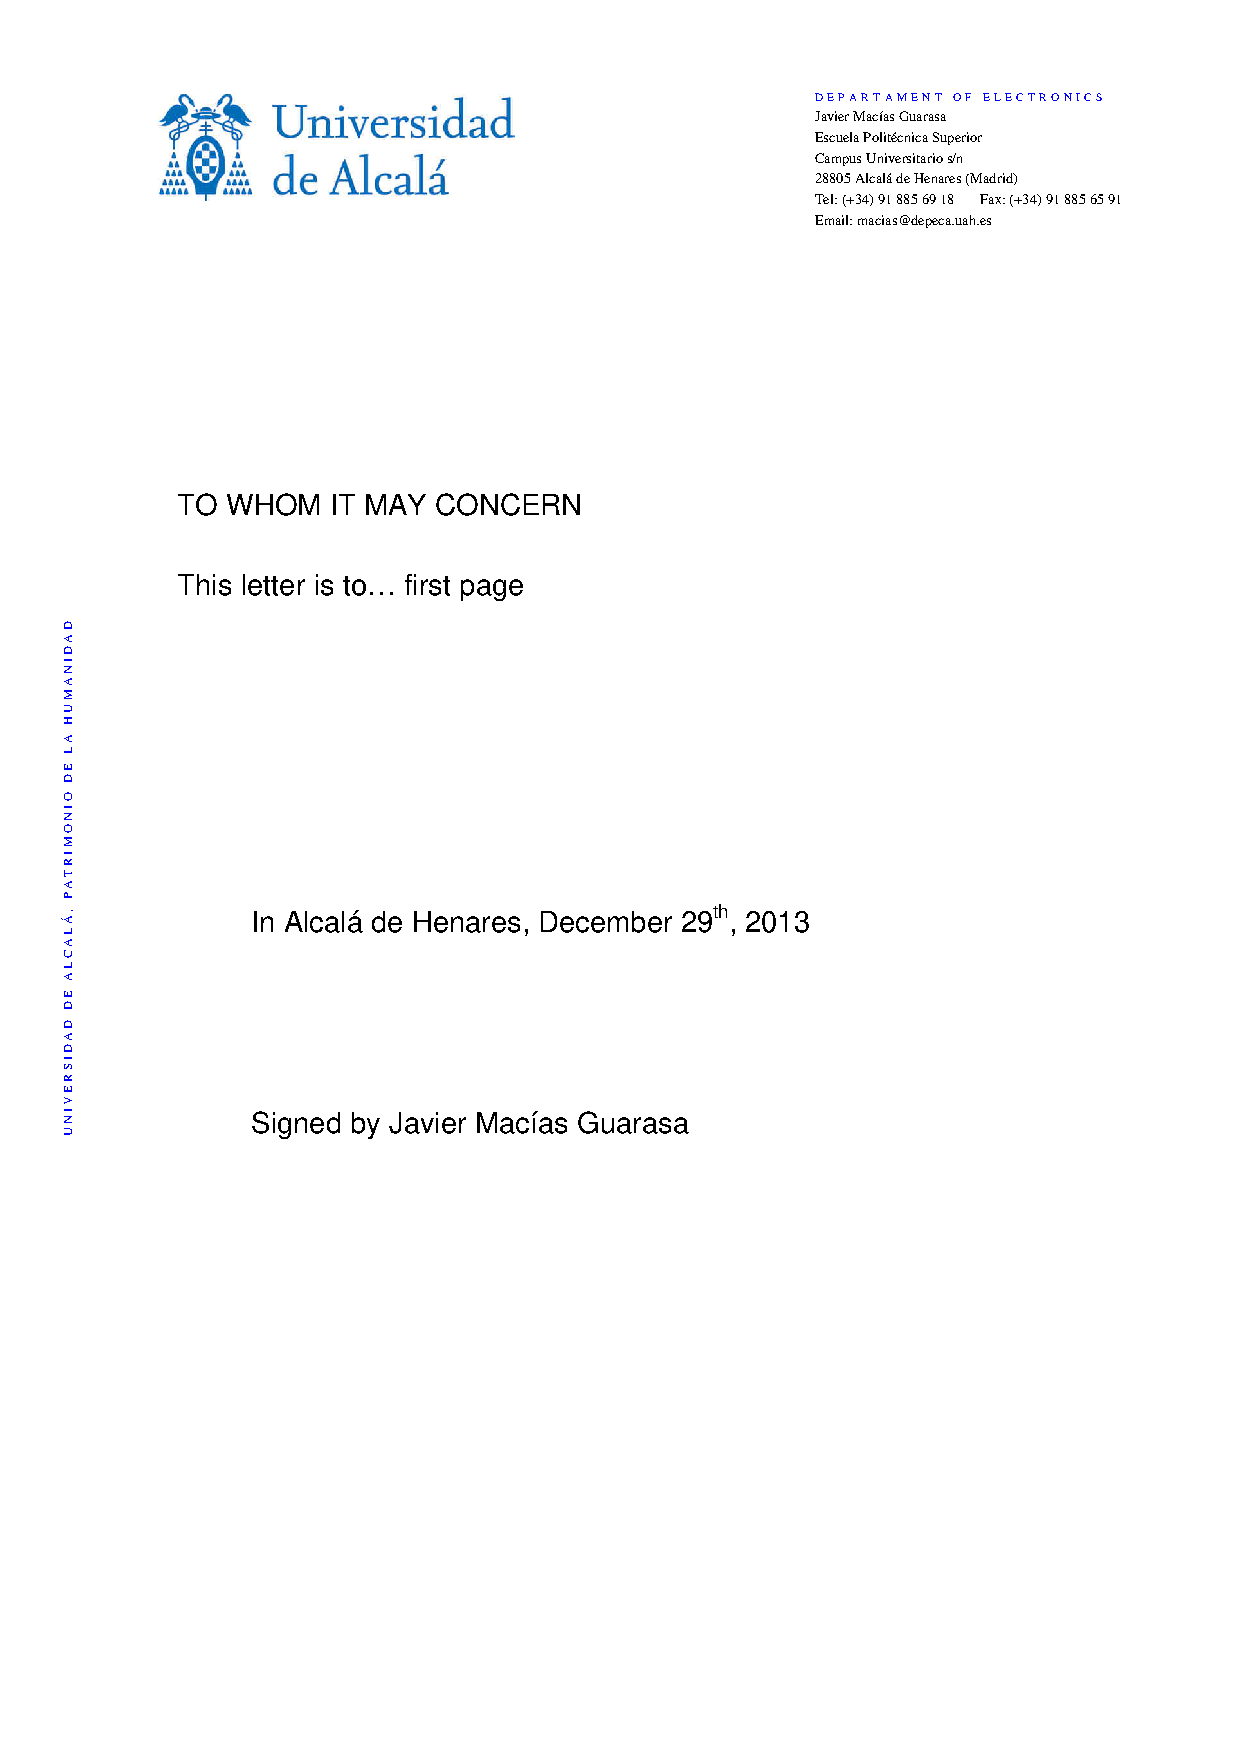
\includepdf[pages=-]{letters/sampleLetter-pages.pdf}   % include all pages of
%                                                 % pdf file
\clearemptydoublepage % You need to add this after including each pdf

%\includepdf[pages=-]{papeleo/vistoBuenoTutorTFM-MUSEA.pdf}   % for TFMs
%\clearemptydoublepage % You need to add this after including each pdf

% Dedication+ackowledgements (dedicatorias+agradecimientos)
%%%%%%%%%%%%%%%%%%%%%%%%%%%%%%%%%%%%%%%%%%%%%%%%%%%%%%%%%%%%%%%%%%%%%%%%%%% 
% 
% Generic template for TFC/TFM/TFG/Tesis
% 
% $Id: dedicatoria.tex,v 1.5 2015/06/05 00:10:35 macias Exp $
% 
% By:
% + Javier Macías-Guarasa. 
% Departamento de Electrónica
% Universidad de Alcalá
% + Roberto Barra-Chicote. 
% Departamento de Ingeniería Electrónica
% Universidad Politécnica de Madrid   
% 
% Based on original sources by Roberto Barra, Manuel Ocaña, Jesús Nuevo,
% Pedro Revenga, Fernando Herránz and Noelia Hernández. Thanks a lot to
% all of them, and to the many anonymous contributors found (thanks to
% google) that provided help in setting all this up.
% 
% See also the additionalContributors.txt file to check the name of
% additional contributors to this work.
% 
% If you think you can add pieces of relevant/useful examples,
% improvements, please contact us at (macias@depeca.uah.es)
% 
% You can freely use this template and please contribute with
% comments or suggestions!!!
% 
%%%%%%%%%%%%%%%%%%%%%%%%%%%%%%%%%%%%%%%%%%%%%%%%%%%%%%%%%%%%%%%%%%%%%%%%%%% 

% 
% This is also courtesy of Roberto Barra
% 
% To center text in a page:
% \topskip0pt
% \vspace*{\fill}
% text
% \vspace*{\fill}

\thispagestyle{empty}

\begin{flushright}

  \topskip0pt
  \vspace*{\fill}

  \textbf{A nuestros alumnos pasados, presentes y futuros\ldots}\\

  \vspace{3cm}

  \emph{``Empieza haciendo lo necesario, luego haz lo posible y de
    pronto empezarás a hacer lo imposible.''}\\ Francisco de Asís

\end{flushright}  

\vspace{4cm}
\vspace*{\fill}

% \clearemptydoublepage



%%% Local Variables:
%%% TeX-master: "../book"
%%% End:
            % EDIT this file or
                                              % comment it out
%%%%%%%%%%%%%%%%%%%%%%%%%%%%%%%%%%%%%%%%%%%%%%%%%%%%%%%%%%%%%%%%%%%%%%%%%%%
%
% Generic template for TFC/TFM/TFG/Tesis
%
% $Id: agradecimientos.tex,v 1.7 2015/06/05 00:10:31 macias Exp $
%
% By:
%  + Javier Macías-Guarasa. 
%    Departamento de Electrónica
%    Universidad de Alcalá
%  + Roberto Barra-Chicote. 
%    Departamento de Ingeniería Electrónica
%    Universidad Politécnica de Madrid   
% 
% Based on original sources by Roberto Barra, Manuel Ocaña, Jesús Nuevo,
% Pedro Revenga, Fernando Herránz and Noelia Hernández. Thanks a lot to
% all of them, and to the many anonymous contributors found (thanks to
% google) that provided help in setting all this up.
%
% See also the additionalContributors.txt file to check the name of
% additional contributors to this work.
%
% If you think you can add pieces of relevant/useful examples,
% improvements, please contact us at (macias@depeca.uah.es)
%
% You can freely use this template and please contribute with
% comments or suggestions!!!
%
%%%%%%%%%%%%%%%%%%%%%%%%%%%%%%%%%%%%%%%%%%%%%%%%%%%%%%%%%%%%%%%%%%%%%%%%%%%

% Use this if you don't like the fancy style
\thispagestyle{empty}

\ifthenelse{\equal{\myLanguage}{english}}
{
  \chapter*{Acknowledgements}
  \label{cha:acknowledgements}
  \markboth{Acknowledgements}{Acknowledgements}
  \addcontentsline{toc}{chapter}{Acknowledgements}
}
{
  \chapter*{Agradecimientos}
  \label{cha:agradecimientos}
  \markboth{Agradecimientos}{Agradecimientos}
  \addcontentsline{toc}{chapter}{Agradecimientos}
}




\begin{FraseCelebre}
  \begin{Frase}
    A todos los que la presente vieren y entendieren.
  \end{Frase}
  \begin{Fuente}
    Inicio de las Leyes Orgánicas. Juan Carlos I
  \end{Fuente}
\end{FraseCelebre}

% ``Más vale un minuto de ilusión que mil horas de
% razonamiento''... (cortesía de Roberto Barra)


Este trabajo es el fruto de muchas horas de trabajo, tanto de los
autores últimos de los ficheros de la distribución como de todos los que
en mayor o menor medida han participado en él a lo largo de su proceso
de gestación.

Mención especial merece Manuel Ocaña, el autor de la primera versión de
las plantillas de proyectos fin de carrera y tesis doctorales usadas en
el Departamento de Electrónica de la Universidad de Alcalá, con
contribuciones de Jesús Nuevo, Pedro Revenga, Fernando Herránz y Noelia
Hernández.

En la versión actual, la mayor parte de las definiciones de estilos de
partida proceden de la tesis doctoral de Roberto Barra-Chicote, con lo
que gracias muy especiales para él.

Añado igualmente a Gonzalo Corral de forma destacada en esta sección por ser el
primero que hizo un PR sobre el repositorio github de la plantilla, y que nos
llevó del arcaico ISO-8859 de bibtex a la normalidad del UTF-8 de biber (que ya
hacía falta).

También damos las gracias a \input{additionalContributors.txt} que nos
han proporcionado secciones completas y ejemplos puntuales de sus
proyectos fin de carrera.

Finalmente, hay incontables contribuyentes a esta plantilla, la mayoría
encontrados gracias a la magia del buscador de Google. Hemos intentado
referenciar los más importantes en los fuentes de la plantilla, aunque
seguro que hemos omitido alguno. Desde aquí les damos las gracias a
todos ellos por compartir su saber con el mundo.


% Back to normal JIC. Use it if you set \pagestyle{myplain} above
%\pagestyle{fancy}

%%% Local Variables:
%%% TeX-master: "../book"
%%% End:


  % EDIT this file or
                                              % comment it out

% If this is the case, include definitions of acronyms (it's
% included before resumen.tex and abstract.tex in case you want
% to use them here
%%%%%%%%%%%%%%%%%%%%%%%%%%%%%%%%%%%%%%%%%%%%%%%%%%%%%%%%%%%%%%%%%%%%%%%%%%%
%
% Generic template for TFC/TFM/TFG/Tesis
%
% $Id: defacronymsgl.tex,v 1.2 2015/06/05 00:10:31 macias Exp $
%
% By:
%  + Javier Macías-Guarasa. 
%    Departamento de Electrónica
%    Universidad de Alcalá
%  + Roberto Barra-Chicote. 
%    Departamento de Ingeniería Electrónica
%    Universidad Politécnica de Madrid   
% 
% Based on original sources by Roberto Barra, Manuel Ocaña, Jesús Nuevo,
% Pedro Revenga, Fernando Herránz and Noelia Hernández. Thanks a lot to
% all of them, and to the many anonymous contributors found (thanks to
% google) that provided help in setting all this up.
%
% See also the additionalContributors.txt file to check the name of
% additional contributors to this work.
%
% If you think you can add pieces of relevant/useful examples,
% improvements, please contact us at (macias@depeca.uah.es)
%
% You can freely use this template and please contribute with
% comments or suggestions!!!
%
%%%%%%%%%%%%%%%%%%%%%%%%%%%%%%%%%%%%%%%%%%%%%%%%%%%%%%%%%%%%%%%%%%%%%%%%%%%

% This file shows some examples for glossary terms

%%%%%%%%%%%%%%%%%%%%%%%%%%%%%%%%%%%%%%%%%%%%%%%%%%%%%%%%%%%%%%%%%%%%%%%%%%%
% BEGIN example of glossary terms definition
%
\newacronym{HMI}{HMI}{Human-Machine Interfaces}
\newacronym{ETTS}{ETTS}{Emotional Text To Speech}
\newacronym{TTS}{TTS}{Text To Speech}
\newacronym{PSOLA}{PSOLA}{Pitch Synchronous OverLap Add}
\newacronym{TDPSOLA}{TD-PSOLA}{Time Domain Pitch Synchronous OverLap Add}
\newacronym{AI}{AI}{Artificial Intelligenge}

\newacronym{SPSS}{SPSS}{Statistical Parametric Speech Synthesis}
\newacronym{VC}{VC}{Voice Conversion}
\newacronym{US}{US}{Unit Selection}
\newacronym{HMM}{HMM}{Hidden Markov Model}
\newacronym{LSP}{LSP}{Line Spectral Pairs}
\newacronym{LPC}{LPC}{Linear Prediction Coefficiens}
\newacronym{LSF}{LSF}{Line Spectral Frequencies}
\newacronym{F0}{F0}{Fundamental Frequency}
\newacronym{MCEP}{MCEP}{Mel Cepstral Coefficients}
\newacronym{MGCEP}{MGCEP}{Mel Generalized Cepstral Coefficients}
\newacronym{MFCC}{MFCC}{Mel Frequency Cepstrum Coefficients}
\newacronym{ASR}{ASR}{Automatic Speech Recognition}
\newacronym{MDL}{MDL}{Minimum Description Length Criterion}
\newacronym{MSD}{MSD}{Multi Space Probability Distributions}
\newacronym{HSMM}{HSMM}{Hidden Semi-Markov Models}
\newacronym{ML}{ML}{Maximum Likelihood}
\newacronym{MLSA}{MLSA}{Mel Log Spectrum Approximation}
\newacronym{MAP}{MAP}{Maximum A Posteriori} 
\newacronym{MLLR}{MLLR}{Maximum Likelihood Linear Regression}
\newacronym{CSMAPLR}{CSMAPLR}{Constrain Structural MAP Linear Regression}
\newacronym{AV}{AV}{Average Voice}

\newacronym{ANN}{ANN}{Artificial Neural Network}

\newacronym{NIST}{NIST}{National Institute of Technology}
\newacronym{SES}{SES}{Spanish Expressive Speech}
\newacronym{EMODB}{EMODB}{Berlin Database of Emotional Speech}

\newacronym{FAUAIBO}{FAU-AIBO}{FAU AIBO Emotion Corpus}

\newacronym{SEV}{SEV}{Spanish Expressive Voices}
\newacronym{AER}{AER}{Automatic Emotion Recognition}
\newacronym{UBEC}{UBEC}{Universal Background Emotion Codebook}

\newacronym{STRAIGHT}{STRAIGHT}{Speech Transformation and Representation using Adaptive Interpolation of weiGHTed spectrum}


\newacronym{DBN}{DBN}{Dynamic Bayesian Network}
\newacronym{SQ}{SQ}{Speech Quality}
\newacronym{EIR}{EIR}{Emotion Identification Rate}
\newacronym{SIR}{SIR}{Speaker Identification Rate}
\newacronym{ES}{ES}{Emotional Strength}

\newacronym{ACCCHARS}{ÁÉÍÓÚÜÑáéíóúüñ}{Long ÁÉÍÓÚÜÑáéíóúüñ}

% In the future version of texlive, we will be able to use longplural
% and shortplural. Right now we must use \newglossaryentry.
%\newacronym[longplural={Systems on a Chip},shortplural={SOCs}]{SOC}{SOC}{System on a Chip}
\newglossaryentry{SOC}{type=\acronymtype,
        name={SOC},
        symbol={},
        sort=soc,
        plural={SOCs},
        firstplural={Systems on a Chip (SOCs)},
        description={System on a Chip},
        descriptionplural={Systems on a Chip}}

%
% END example of glossary terms definition
%%%%%%%%%%%%%%%%%%%%%%%%%%%%%%%%%%%%%%%%%%%%%%%%%%%%%%%%%%%%%%%%%%%%%%%%%%%


%%% Local Variables:
%%% TeX-master: "../book"
%%% End:
            % EDIT this file or
                                              % comment it out if you do
                                              % not use acronyms

% If this is the case, include definitions of acronyms (it's
% included before resumen.tex and abstract.tex in case you want
% to use them there
%%%%%%%%%%%%%%%%%%%%%%%%%%%%%%%%%%%%%%%%%%%%%%%%%%%%%%%%%%%%%%%%%%%%%%%%%%%
%
% Generic template for TFC/TFM/TFG/Tesis
%
% $Id: defsymbolsgl.tex,v 1.2 2015/06/05 00:10:37 macias Exp $
%
% By:
%  + Javier Macías-Guarasa. 
%    Departamento de Electrónica
%    Universidad de Alcalá
%  + Roberto Barra-Chicote. 
%    Departamento de Ingeniería Electrónica
%    Universidad Politécnica de Madrid   
% 
% Based on original sources by Roberto Barra, Manuel Ocaña, Jesús Nuevo,
% Pedro Revenga, Fernando Herránz and Noelia Hernández. Thanks a lot to
% all of them, and to the many anonymous contributors found (thanks to
% google) that provided help in setting all this up.
%
% See also the additionalContributors.txt file to check the name of
% additional contributors to this work.
%
% If you think you can add pieces of relevant/useful examples,
% improvements, please contact us at (macias@depeca.uah.es)
%
% You can freely use this template and please contribute with
% comments or suggestions!!!
%
%%%%%%%%%%%%%%%%%%%%%%%%%%%%%%%%%%%%%%%%%%%%%%%%%%%%%%%%%%%%%%%%%%%%%%%%%%%

% These ones for the symbols glossary

%%%%%%%%%%%%%%%%%%%%%%%%%%%%%%%%%%%%%%%%%%%%%%%%%%%%%%%%%%%%%%%%%%%%%%%%%%%
% BEGIN example of symbols definition
%
\newglossaryentry{ohm}{type=symbols,
        name={\ensuremath{\Omega}},
        symbol={\ensuremath{\Omega}}, 
        sort=ohm,
        description=unit of electrical resistance}

\newglossaryentry{angstrom}{type=symbols,
        name={\AA},
        symbol={\AA},
        sort=angstrom,
        description={non-SI unit of length}}

\newglossaryentry{xdet}{type=symbols,
        name={\ensuremath{x(t)}},
        symbol={\ensuremath{x(t)}},
        sort=xdet,
        description={Audio signal}}

\newglossaryentry{xidet}{type=symbols,
        name={\ensuremath{x_i(t)}},
        symbol={\ensuremath{x_i(t)}},
        sort=xidet,
        description={Audio signal captured at microphone $i$}}

\newglossaryentry{condindep}{type=symbols,
        name={\ensuremath{\ci}},
        symbol={\ensuremath{\ci}}, 
        sort=conditionalindependence,
        description=conditional independence}

%
% END example of symbols definition
%%%%%%%%%%%%%%%%%%%%%%%%%%%%%%%%%%%%%%%%%%%%%%%%%%%%%%%%%%%%%%%%%%%%%%%%%%%

%%% Local Variables:
%%% TeX-master: "../book"
%%% End:
              % EDIT this file or
                                              % comment it out if you do
                                              % not use acronyms

% Now include resumen and abstract
%%%%%%%%%%%%%%%%%%%%%%%%%%%%%%%%%%%%%%%%%%%%%%%%%%%%%%%%%%%%%%%%%%%%%%%%%%%
%
% Generic template for TFC/TFM/TFG/Tesis
%
% $Id: resumen.tex,v 1.9 2015/06/05 00:10:31 macias Exp $
%
% By:
%  + Javier Macías-Guarasa. 
%    Departamento de Electrónica
%    Universidad de Alcalá
%  + Roberto Barra-Chicote. 
%    Departamento de Ingeniería Electrónica
%    Universidad Politécnica de Madrid   
% 
% Based on original sources by Roberto Barra, Manuel Ocaña, Jesús Nuevo,
% Pedro Revenga, Fernando Herránz and Noelia Hernández. Thanks a lot to
% all of them, and to the many anonymous contributors found (thanks to
% google) that provided help in setting all this up.
%
% See also the additionalContributors.txt file to check the name of
% additional contributors to this work.
%
% If you think you can add pieces of relevant/useful examples,
% improvements, please contact us at (macias@depeca.uah.es)
%
% You can freely use this template and please contribute with
% comments or suggestions!!!
%
%%%%%%%%%%%%%%%%%%%%%%%%%%%%%%%%%%%%%%%%%%%%%%%%%%%%%%%%%%%%%%%%%%%%%%%%%%%

\chapter*{Resumen}
\label{cha:resumen}
\markboth{Resumen}{Resumen}

\addcontentsline{toc}{chapter}{Resumen}

Este documento ha sido generado con una plantilla para memorias de
trabajos fin de carrera, fin de máster, fin de grado y tesis
doctorales. Está especialmente pensado para su uso en la Universidad de
Alcalá, pero debería ser fácilmente extensible y adaptable a otros casos
de uso. En su contenido se incluyen las instrucciones generales para
usarlo, así como algunos ejemplos de elementos que pueden ser de
utilidad. Si tenéis problemas, sugerencias o comentarios sobre el mismo,
dirigidlas por favor a \contactauthor.

\textbf{Palabras clave:} \myThesisKeywords.

%%% Local Variables:
%%% TeX-master: "../book"
%%% End:


                  % EDIT this file
%%%%%%%%%%%%%%%%%%%%%%%%%%%%%%%%%%%%%%%%%%%%%%%%%%%%%%%%%%%%%%%%%%%%%%%%%%%
%
% Generic template for TFC/TFM/TFG/Tesis
%
% $Id: abstract.tex,v 1.9 2015/06/05 00:10:31 macias Exp $
%
% By:
%  + Javier Macías-Guarasa. 
%    Departamento de Electrónica
%    Universidad de Alcalá
%  + Roberto Barra-Chicote. 
%    Departamento de Ingeniería Electrónica
%    Universidad Politécnica de Madrid   
% 
% Based on original sources by Roberto Barra, Manuel Ocaña, Jesús Nuevo,
% Pedro Revenga, Fernando Herránz and Noelia Hernández. Thanks a lot to
% all of them, and to the many anonymous contributors found (thanks to
% google) that provided help in setting all this up.
%
% See also the additionalContributors.txt file to check the name of
% additional contributors to this work.
%
% If you think you can add pieces of relevant/useful examples,
% improvements, please contact us at (macias@depeca.uah.es)
%
% You can freely use this template and please contribute with
% comments or suggestions!!!
%
%%%%%%%%%%%%%%%%%%%%%%%%%%%%%%%%%%%%%%%%%%%%%%%%%%%%%%%%%%%%%%%%%%%%%%%%%%%

\chapter*{Abstract}
\label{cha:abstract}

\addcontentsline{toc}{chapter}{Abstract}

Since Hertz demonstrated in 1887 the possibility of using devices for the transmission of electromagnetic waves through an open medium such as air, the need arose to be able to characterize their behavior reliably.

Over time, measurement standards have evolved to increase the accuracy of measurements.  At the core of the motivation of this work is the creation of an algorithm capable of representing far-field radiation diagrams from near-field measurements that will allow the High Technology and Homologation Center (CATECHOM) of the Polytechnic School of the University of Alcalá to renew the current software available since 1999.


\textbf{Keywords:} \myThesisKeywordsEnglish.

%%% Local Variables:
%%% TeX-master: "../book"
%%% End:


                 % EDIT this file

% Just for TFGs/PFCs at UAH, I do nothing and leave to the author the
% inclusion of the file
%%%%%%%%%%%%%%%%%%%%%%%%%%%%%%%%%%%%%%%%%%%%%%%%%%%%%%%%%%%%%%%%%%%%%%%%%%%%
%
% Generic template for TFC/TFM/TFG/Tesis
%
% $Id: resumen-extendido.tex,v 1.6 2015/06/05 00:10:31 macias Exp $
%
% By:
%  + Javier Macías-Guarasa. 
%    Departamento de Electrónica
%    Universidad de Alcalá
%  + Roberto Barra-Chicote. 
%    Departamento de Ingeniería Electrónica
%    Universidad Politécnica de Madrid   
% 
% Based on original sources by Roberto Barra, Manuel Ocaña, Jesús Nuevo,
% Pedro Revenga, Fernando Herránz and Noelia Hernández. Thanks a lot to
% all of them, and to the many anonymous contributors found (thanks to
% google) that provided help in setting all this up.
%
% See also the additionalContributors.txt file to check the name of
% additional contributors to this work.
%
% If you think you can add pieces of relevant/useful examples,
% improvements, please contact us at (macias@depeca.uah.es)
%
% You can freely use this template and please contribute with
% comments or suggestions!!!
%
%%%%%%%%%%%%%%%%%%%%%%%%%%%%%%%%%%%%%%%%%%%%%%%%%%%%%%%%%%%%%%%%%%%%%%%%%%%

\ifthenelse{\equal{\myLanguage}{english}}
{
\chapter*{Extended Abstract}
\label{cha:resumen-extendido}
\markboth{Extended Abstract}{Extended Abstract}

\addcontentsline{toc}{chapter}{Extended Abstract}
}
{
\chapter*{Resumen extendido}
\label{cha:resumen-extendido}
\markboth{Resumen extendido}{Resumen extendido}

\addcontentsline{toc}{chapter}{Resumen extendido}
}

Con un máximo de cuatro o cinco páginas. Se supone que sólo está
definido como obligatorio para los TFGs y PFCs de UAH.

%%% Local Variables:
%%% TeX-master: "../book"
%%% End:


       % EDIT this file

% Now include toc and list of figures+tables
\input{cover/toc+lof+lot.tex}                 % DO NOT TOUCH THIS LINE!

% If you want to include additional listings, you can use the float
% package. As an example, I include here the listing of source code
% snippets and algorithms (you have some examples in
% appendix/manual.tex)
\input{cover/extralistings.tex}               % Edit this file or
                                              % comment it out

% Now include list of acronyms and options (if this is the case)
%%%%%%%%%%%%%%%%%%%%%%%%%%%%%%%%%%%%%%%%%%%%%%%%%%%%%%%%%%%%%%%%%%%%%%%%%%%
%
% Generic template for TFC/TFM/TFG/Tesis
%
% $Id: acronymsgl.tex,v 1.8 2015/06/05 00:10:31 macias Exp $
%
% By:
%  + Javier Macías-Guarasa. 
%    Departamento de Electrónica
%    Universidad de Alcalá
%  + Roberto Barra-Chicote. 
%    Departamento de Ingeniería Electrónica
%    Universidad Politécnica de Madrid   
% 
% Based on original sources by Roberto Barra, Manuel Ocaña, Jesús Nuevo,
% Pedro Revenga, Fernando Herránz and Noelia Hernández. Thanks a lot to
% all of them, and to the many anonymous contributors found (thanks to
% google) that provided help in setting all this up.
%
% See also the additionalContributors.txt file to check the name of
% additional contributors to this work.
%
% If you think you can add pieces of relevant/useful examples,
% improvements, please contact us at (macias@depeca.uah.es)
%
% You can freely use this template and please contribute with
% comments or suggestions!!!
%
%%%%%%%%%%%%%%%%%%%%%%%%%%%%%%%%%%%%%%%%%%%%%%%%%%%%%%%%%%%%%%%%%%%%%%%%%%%

% You can change the way the entries appear the first time they are
% used. I've used italics by default. I found a problem if using this:
% LaTeX adds an extra space after the acronym, so I'm commenting it out
% (if you find a solution, please let me know)
%\defglsdisplayfirst[\acronymtype]{\textit{#1}} % EDIT this if required

% This may lead to problems... I don't know how to fix it in case the
% column for acronym is wider than 0.3\linewidth
\setlength{\glsdescwidth}{0.7\linewidth}       % EDIT this if required

% Set language specific definitions...
\ifthenelse{\equal{\myLanguage}{english}}
{
\printglossary[type=\acronymtype,style=super,nonumberlist=true,title=List of Acronyms,toctitle=List of Acronyms]
\addcontentsline{toc}{chapter}{List of Acronyms}
}
{
\printglossary[type=\acronymtype,style=super,nonumberlist=true,title=Lista de acrónimos,toctitle=Lista de acrónimos]
\addcontentsline{toc}{chapter}{Lista de acrónimos}
}


%%% Local Variables:
%%% TeX-master: "../book"
%%% End:


               % EDIT this file or
                                              % comment it out if you do
                                              % not use acronyms

% Now include symbols of symbols and options (if this is the case)
%%%%%%%%%%%%%%%%%%%%%%%%%%%%%%%%%%%%%%%%%%%%%%%%%%%%%%%%%%%%%%%%%%%%%%%%%%%
%
% Generic template for TFC/TFM/TFG/Tesis
%
% $Id: symbolsgl.tex,v 1.8 2015/06/05 00:10:37 macias Exp $
%
% By:
%  + Javier Macías-Guarasa. 
%    Departamento de Electrónica
%    Universidad de Alcalá
%  + Roberto Barra-Chicote. 
%    Departamento de Ingeniería Electrónica
%    Universidad Politécnica de Madrid   
% 
% Based on original sources by Roberto Barra, Manuel Ocaña, Jesús Nuevo,
% Pedro Revenga, Fernando Herránz and Noelia Hernández. Thanks a lot to
% all of them, and to the many anonymous contributors found (thanks to
% google) that provided help in setting all this up.
%
% See also the additionalContributors.txt file to check the name of
% additional contributors to this work.
%
% If you think you can add pieces of relevant/useful examples,
% improvements, please contact us at (macias@depeca.uah.es)
%
% You can freely use this template and please contribute with
% comments or suggestions!!!
%
%%%%%%%%%%%%%%%%%%%%%%%%%%%%%%%%%%%%%%%%%%%%%%%%%%%%%%%%%%%%%%%%%%%%%%%%%%%


% Set language specific definitions...
\ifthenelse{\equal{\myLanguage}{english}}
{
  \printglossary[type=symbols,style=super,nonumberlist=true,title=List of Symbols,toctitle=List of Symbols]
  \addcontentsline{toc}{chapter}{List of Symbols}
}
{
  \printglossary[type=symbols,style=super,nonumberlist=true,title=Lista de símbolos,title=Lista de símbolos,toctitle=Lista de símbolos]
  \addcontentsline{toc}{chapter}{Lista de símbolos}
}


%%% Local Variables:
%%% TeX-master: "../book"
%%% End:
                 % EDIT this file or
                                              % comment it out if you do
                                              % not use acronyms

%
% END within-document configuration, frontpage and cover pages generation
%%%%%%%%%%%%%%%%%%%%%%%%%%%%%%%%%%%%%%%%%%%%%%%%%%%%%%%%%%%%%%%%%%%%%%%%%%%


%%%%%%%%%%%%%%%%%%%%%%%%%%%%%%%%%%%%%%%%%%%%%%%%%%%%%%%%%%%%%%%%%%%%%%%%%%%
% Now start text and numbering for mainmatter (chapter+appendices)
%%%%%%%%%%%%%%%%%%%%%%%%%%%%%%%%%%%%%%%%%%%%%%%%%%%%%%%%%%%%%%%%%%%%%%%%%%%
\mainmatter                                       % DO NOT TOUCH THIS LINE!
\deactivatetilden                                 % DO NOT TOUCH THIS LINE!


%%%%%%%%%%%%%%%%%%%%%%%%%%%%%%%%%%%%%%%%%%%%%%%%%%%%%%%%%%%%%%%%%%%%%%%%%%%
%%%%%%%%%%%%%%%%%%%%%%%%%%%%%%%%%%%%%%%%%%%%%%%%%%%%%%%%%%%%%%%%%%%%%%%%%%%
%%%%%%%%%%%%%%%%%%%%%%%%%%%%%%%%%%%%%%%%%%%%%%%%%%%%%%%%%%%%%%%%%%%%%%%%%%%
%%%%%%%%%%%%%%%%%%%%%%%%%%%%%%%%%%%%%%%%%%%%%%%%%%%%%%%%%%%%%%%%%%%%%%%%%%%
%%%%%%%%%%%%%%%%%%%%%%%%%%%%%%%%%%%%%%%%%%%%%%%%%%%%%%%%%%%%%%%%%%%%%%%%%%%
%%%%%%%%%%%%%%%%%%%%%%%%%%%%%%%%%%%%%%%%%%%%%%%%%%%%%%%%%%%%%%%%%%%%%%%%%%%
%%%%%%%%%%%%%%%%%%%%%%%%%%%%%%%%%%%%%%%%%%%%%%%%%%%%%%%%%%%%%%%%%%%%%%%%%%%
% BEGIN Normal chapters. Edit/modify all within this section
%
% I don't recommend it, but if you want to define "parts", use this...
% BEWARE: I didn't write the english dependent code
%\part*{Memoria}
%\label{part:memoria}

%%%%%%%%%%%%%%%%%%%%%%%%%%%%%%%%%%%%%%%%%%%%%%%%%%%%%%%%%%%%%%%%%%%%%%%%%%% 
% 
% Generic template for TFC/TFM/TFG/Tesis
% 
% By:
%  + Javier Macías-Guarasa.
%    Departamento de Electrónica
%    Universidad de Alcalá
%  + Roberto Barra-Chicote.
%    Departamento de Ingeniería Electrónica
%    Universidad Politécnica de Madrid
% 
% By: + Javier Macías-Guarasa. Departamento de Electrónica Universidad de Alcalá + Roberto Barra-Chicote. Departamento de Ingeniería Electrónica Universidad Politécnica de Madrid
% 
% Based on original sources by Roberto Barra, Manuel Ocaña, Jesús Nuevo, Pedro Revenga, Fernando Herránz and Noelia Hernández. Thanks a lot to all of them, and to the many anonymous contributors found (thanks to google) that provided help in setting all this up.
% 
% See also the additionalContributors.txt file to check the name of additional contributors to this work.
% 
% If you think you can add pieces of relevant/useful examples, improvements, please contact us at (macias@depeca.uah.es)
% 
% You can freely use this template and please contribute with comments or suggestions!!!
% 
%%%%%%%%%%%%%%%%%%%%%%%%%%%%%%%%%%%%%%%%%%%%%%%%%%%%%%%%%%%%%%%%%%%%%%%%%%% 

\chapter{Introducción}
\label{cha:introduccion}

\begin{FraseCelebre}
  \begin{Frase}
    Desocupado lector, sin juramento me podrás creer que quisiera que este libro [...] fuera el más hermoso, el más gallardo y más discreto que pudiera imaginarse\footnote{Tomado de ejemplos del proyecto \texis{}.}.
  \end{Frase}
  \begin{Fuente}
    Miguel de Cervantes, Don Quijote de la Mancha
  \end{Fuente}
\end{FraseCelebre}


\section{Presentación}
\label{sec:presentacion}

Esta plantilla\footnote{Asegúrate de compilar de nuevo el documento (como cuenta la sección~\ref{sec:compilacion}), para verificar que todo funciona y por si ha habido algún cambio en los fuentes que no está reflejado en los pdf de ejemplo precompilados.} pretende proporcionar un conjunto de estilos consistentes y unificados para cubrir las necesidades de generación de memorias \LaTeX{} para cada uno de los TFCs/TFMs/TFGs y tesis doctorales que se generen en la Escuela Politécnica Superior de la Universidad de Alcalá\footnote{También se incluye la definición para las tesis de la Escuela Técnica Superior de Ingenieros de Telecomunicación de la Universidad Politécnica de Madrid. La extensión a los TFGs de la misma es sencilla, aunque no se ha realizado por el momento.}.

Para utilizar la plantilla se han generado algunos capítulos genéricos en los que se han incluido secciones ``tutoriales'', en la que se explican algunas de sus características y se muestran ejemplos de elementos típicos que pueden ser de utilidad (pero sin el objetivo de que esto sea una guía de \LaTeX{}).

Igualmente se proporciona un modelo simplificado de un anteproyecto (para el caso de los TFCs/TFMs/TFGs), así como parte de la documentación que hay que presentar para la defensa de los TFGs/TFMs de la Universidad de Alcalá.



\section{Uso de la plantilla}
\label{sec:uso-generico-de}


\subsection{Prerrequisitos}
\label{sec:prerrequisitos}

Para usar la plantilla tal y como está definida, hace falta disponer de una serie de paquetes de estilos \LaTeX{} (ficheros \texttt{.sty}), todos ellos definidos en el fichero \texttt{Config/preamble.tex}.

No vamos a hacer un listado de todos lo necesarios (sería demasiado largo\footnote{Los que suelen no estar instalados en un ubuntu estándar son \texttt{texlive-publishers}, \texttt{texlive-science}}), pero en la mayoría de distribuciones GNU/Linux serán fáciles de conseguir en caso de que la compilación genere un error de fichero no encontrado. Si os sucede, buscadlos en alguno de los paquetes \texttt{texlive-*}. En caso de no encontrarlos, una búsqueda en google (que con casi total seguridad referenciará a alguna página en CTAN) os dará el enlace a la descarga correspondiente. A partir de ahí, su inclusión en directorios locales será suficiente.
% (como por ejemplo hemos tenido que hacer con el paquete \texttt{background}, incluido en la distribución en el directorio \texttt{sty/background}). Lo más cómodo es hacer una instalación del \texttt{texlive-full}.

Igualmente será necesario tener instaladas una serie de utilidades y aplicaciones:

\begin{itemize}
  \item En Linux

        \begin{itemize}
          \item \texttt{make}, si se quiere utilizar la facilidad del \texttt{Makefile} suministrado. Está disponible en todas las distribuciones GNU/Linux.
          \item \texttt{rubber}, si se quiere utilizar la prestación de compilación de código \LaTeX{} incluida en el \texttt{Makefile}. Debería estar disponible en cualquier distribución GNU/Linux, pero si no es así, puedes optar por descargarla, o bien usar la alternativa de \texttt{latexmk} (para el que también se incluyen targets específicos en el \texttt{Makefile} suministrado).
          \item \texttt{dia}, si se quiere utilizar el ejemplo proporcionado de generación de esquemas con dicha herramienta.
          \item \texttt{epspdf}, si se quiere utilizar la facilidad de la conversión automática de ficheros \texttt{eps} a \texttt{pdf} (también se usa en la conversión de ficheros \texttt{.dia}).
          \item \texttt{makeglossaries}, si se quiere utilizar la prestación de manejo de listas de acrónimos y variables. Suele estar en el paquete \texttt{texlive-latex-extra} en distribuciones basadas en Debian (como ubuntu y derivados).
          % \item \texttt{latexdiff} y \texttt{latexpand}, si se quiere utilizar la prestación de generación de ficheros pdf con control de cambios. El primero suele ser un paquete independiente, y el segundo suele estar en el paquete \texttt{texlive-extra-utils}.
        \end{itemize}

  \item En Windows (os cuento la configuración que he probado en algún momento):

        \begin{itemize}
          \item \texttt{miktex} como sistema de compilación \LaTeX{}, diciéndole que instale todo lo que necesite.
          \item \texttt{TeXstudio} o \texttt{TeXMaker} como editor.
          \item Para usar glossaries, echadle un ojo a \url{https://tex.stackexchange.com/questions/156270/has-anyone-managed-to-use-glossaries-with-texstudio-on-windows}. Os copio aquí info que nos han pasado al respecto (gracias Cristina Losada): En Texmaker se puede configurar la “Compilacion rápida” con los comandos que queramos. Eso está en el menú Opciones a Configurar Texmaker, y a la izquierda de la ventana que sale hay que elegir “Compilación rápida”. Hay las opciones típicas, y además permite usar los comandos elegidos por el usuario. Ahí yo tengo esta configuración (compila con pdflatex, llama además a bibtex y makeglossaries y al final muestra el pdf): \texttt{pdflatex -synctex=1 -interaction=nonstopmode \%.tex|bibtex \%|makeglossaries \%|pdflatex -synctex=1 -interaction=nonstopmode \%.tex|pdflatex -synctex=1 -interaction=nonstopmode \%.tex|}''\texttt{C:/Program Files (x86)/Adobe/Acrobat Reader DC/Reader/AcroRd32.exe}''\texttt{ \%.pdf}
    \item \texttt{make}, si se quiere utilizar la facilidad del \texttt{Makefile} suministrado. Hay varias opciones y que necesita un intérprete de comandos (es posible que con el nuevo WSL sea más fácil todavía).
  \end{itemize}
\end{itemize}

\subsection{Compilación}
\label{sec:compilacion}

Para facilitar la generación del documento se incluye un \texttt{Makefile} relativamente sencillo. No somos expertos ni en \texttt{make} ni en \LaTeX, con lo que seguro que no es el mejor de los \texttt{Makefiles} del mundo, pero creemos que hace su función.

El \texttt{Makefile} tiene las siguientes características y prestaciones:

\begin{itemize}

  \item Hace uso de la herramienta \texttt{rubber}. En caso de no disponer de ella, puede usarse \texttt{latexmk} (hay targets específicos de ejemplo para ese caso), pero esta última herramienta no ha sido probada intensivamente. Si no se dispone de ninguna de ellas, habría que generar la estructura típica de compilación: (al estilo \texttt{pdflatex + bibtex + pdflatex + pdflatex}).
  \item Soporta la generación automática de ficheros \texttt{pdf} a partir de los \texttt{dia} y \texttt{svg} (se han elegido estos a modo de ejemplo, pero se puede adaptar fácilmente a otras necesidades).
  \item Genera la información de listas de acrónimos y símbolos con la herramienta \texttt{makeglossaries}. Es imprescindible tenerla instalada si se desea usar esa capacidad.
  \item Soporta los targets:
        \begin{itemize}
          \item \texttt{all} (que es la opción predeterminada si se ejecuta \texttt{make} sin más argumentos), que genera el fichero \texttt{book.pdf} correspondiente, usando \texttt{rubber} y \texttt{makeglossaries}. No nos hemos planteado la generación de ficheros en otros formatos.
          \item \texttt{all\_latexmk}, que genera el fichero \texttt{book.pdf} correspondiente, usando \texttt{latexmk} y \texttt{makeglossaries}. Si ésta es tu opción, sustituye el target \texttt{all} por éste, para facilitarte la compilación.

          \item \texttt{tar}, que genera un fichero \texttt{tgz} que contiene todo lo necesario para la distribución de la plantilla.
          \item \texttt{clean}, que borra todos los ficheros temporales usando \texttt{rubber} (para simplificar los targets, la limpieza se hace tanto para los temporales de generación del \texttt{book.pdf} como los del \texttt{anteproyecto.pdf}).
          \item \texttt{clean\_latexmk}, que borra todos los ficheros temporales usando \texttt{latexmk}. Si ésta es tu opción, sustituye el target \texttt{clean} por éste, para facilitarte la compilación (para simplificar los targets, la limpieza se hace tanto para los temporales de generación del \texttt{book.pdf} como los del \texttt{anteproyecto.pdf}).

          \item \texttt{bare}, que deja razonablemente limpios los ficheros de los capítulos y apéndices, además de borrar los gráficos del directorio \texttt{figures} y \texttt{diagrams}, para que sea más fácil comenzar a editar. \textbf{OJO: HAY CONSECUENCIAS NEGATIVAS NO DESPRECIABLES PORQUE SE BORRARÁ TODO LO QUE TENGAS EN ESOS DIRECTORIOS Y SÓLO DEBERÍA HACERSE CUANDO VAYAMOS A EMPEZAR A ESCRIBIR NUESTRA MEMORIA DEL TRABAJO REALIZADO}.

          \item \texttt{backup-chapters}, que hace un backup de los ficheros que hay en los directorios \texttt{chapters} y \texttt{appendix}, creando directorios cuyo nombre es la fecha y hora actuales y que se crean bajo los anteriores. No debería hacer falta si usas un buen sistema de control de versiones.
        \end{itemize}

\end{itemize}


\subsection{Detalles específicos para sistemas basados en MacOS}
\label{sec:detall-espec-para}

Esta información es cortesía de Carlos Cruz, que se encontró con un problema en la generación de la lista de acrónimos. Copio a continuación los detalles al respecto, aunque estará desactualizado en cuanto a los números de versiones según pasen los años.

Hemos encontrado que la lista de acrónimos y/o símbolos no se genera en el entorno macOS. Recomendamos seguir las siguientes instrucciones para solucionar este problema:

\begin{itemize}
  \item Tener el SO actualizado a la última versión. Actualmente (marzo de 2020) MacOS Catalina versión 10.15.2
  \item Instalar la última versión de MacTeX-2019. Esta distribución requiere Mac OS 10.12, Sierra, o superior y funciona con procesadores Intel (disponible en \href{http://tug.org/mactex/mactex-download.html}{http://tug.org/mactex/mactex-download.html}).
  \item Trabajar en el entorno Texshop version 4.44: \href{https://pages.uoregon.edu/koch/texshop/}{https://pages.uoregon.edu/koch/texshop/}.
\end{itemize}

Si compilamos la plantilla en el entorno Texshop, comprobamos que los listados de glosario y/o símbolos no se compilan con ninguno de los Typeset: Latex, Lualatex, Xelatex o pdflatexmk.

Recomendamos inicialmente compilar por Terminal:

\begin{itemize}
  \item pdflatex “nombre del fichero.tex” (compilar dos veces)
  \item makeglossaries “nombre del fichero”
  \item pdflatex “nombre del fichero” (compilar dos veces)
\end{itemize}

De esta forma, se crea correctamente la lista de acrónimos y símbolos. A continuación, se puede trabajar con futuros cambios en el proyecto mediante Texshop compilando Latex. Si quiere actualizar o modificar la lista de acrónimos y/o símbolos nuevamente, recomendamos borrar todos los ficheros salvo el fichero book.tex y compilar de nuevo por consola para crear la lista correctamente.



\subsection{Estructura del documento generado por la plantilla}
\label{sec:estr-del-docum}

La plantilla definida presenta la siguiente estructura:

\begin{itemize}

  \item Portada y página de información sobre el trabajo, que será dependiente del tipo de trabajo y la titulación. Se genera automáticamente a partir de la información definida en la sección~\ref{sec:definicion-del-tipo}

  \item Ficheros pdf insertados, que aplican en algunos de los tipos de documentos (por ejemplo en las tesis doctorales).

  \item Dedicatoria, con un ejemplo incluido en el fichero \texttt{dedication/dedicatoria.tex}.
  \item Agradecimientos, con un ejemplo incluido en el fichero \texttt{dedication/agradecimientos.tex}.


  \item Resumen en español, con un ejemplo incluido en el fichero \texttt{abstract/resumen.tex}.
  \item Resumen en inglés, con un ejemplo incluido en el fichero \texttt{abstract/abstract.tex}.
  \item Resumen extendido en español (opcional en algunos tipos de documento), con un ejemplo incluido en el fichero \texttt{abstract/resumen-extendido.tex}.

  \item Índice de contenidos, índice de figuras e índice de tablas.
  \item Índices adicionales, de los que se incluye un ejemplo de listado específico en el fichero \texttt{cover/extralistings.tex}, que incluye el listado de fragmentos de código fuente definidos en el \texttt{appendix/manual.tex}, así como un nuevo listado de vídeos que incluimos en 2023 tras una petición recibida al respecto.

  \item Listado de acrónimos utilizados, que se definen en el fichero \texttt{acronyms/defacronymsgl.tex} (con opciones adicionales de configuración en \texttt{acronyms/acronymsgl.tex}), y del que incluimos más información en la sección~\ref{sec:uso-de-acronimos}.
  \item Listado de símbolos utilizados, que se definen en el fichero \texttt{symbols/defsymbolsgl.tex} (con opciones adicionales de configuración en \texttt{symbols/symbolsgl.tex}), y del que incluimos más información en la sección~\ref{sec:simbolos}.


  \item Capítulos del documento, del que hay varios ejemplos que siguen la estructura típica (introducción, estudio teórico, desarrollo, resultados y conclusiones.

  \item Pliego de condiciones y presupuesto, opcionales en función del tipo de documento que se genere (se incluyen un par de ejemplos del trabajo fin de carrera de Jesús Martínez en los ficheros \texttt{pliego/pliego-ejemplo.tex} y \texttt{presupuesto/presupuesto-ejemplo.tex}. Es un trabajo antiguo y es necesario que busquéis esquemas y contenidos actualizados para estos capítulos.

  \item Bibliografía, de la que se puede cambiar el estilo utilizado y los ficheros \texttt{.bib} en el fichero \texttt{biblio/bibliography.tex} (en el que hay que definir la lista de ficheros de bibliografía que se usarán (variables \texttt{\textbackslash{}mybibfileOne}, \texttt{\textbackslash{}mybibfileTwo}, ...).

  \item Apéndices, de los que ahora se incluyen dos ejemplos en los ficheros \texttt{appendix/manual.tex} (que sirve de pretexto para mostrar cómo se insertan fragmentos de código fuente), y \texttt{appendix/herramientas.tex}.
  \item Contraportada.
\end{itemize}

Por supuesto, modificad la estructura para que encaje en las directrices que tengáis al respecto de cómo documentar vuestro trabajo.


\subsection{Definiciones específicas del tipo de documento}
\label{sec:definicion-del-tipo}

Para comenzar a usar la plantilla es fundamental revisar el fichero \texttt{book.tex} en el que se incluyen todos los detalles genéricos de la estructura usada en el documento, con comentarios que esperamos que os ayuden a entenderlo. Si sois de los impacientes, basta con que comencéis por la parte en la que se incluyen los distintos capítulos (buscad la parte de los \texttt{\textbackslash{}input\{chapters/*.tex\}}).

El fichero de configuración más importantes es el \texttt{Config/myconfig.tex} en el que se incluyen elementos para determinar la configuración específica de tu documento y que es de donde se toman los datos para las muchas automatizaciones del proceso de generación. El primero de ellos (para facilitar la generación de documentos en español o inglés), es el que define el idioma que vas a utilizar. Para seleccionarlo, basta con asignar \texttt{spanish} o \texttt{english} a la variable \texttt{\textbackslash{}myLanguage}. A partir de ella, el sistema generará las cabeceras y títulos adecuados a cada una.

Igualmente, tendréis que definir las siguientes variables sobre el tipo de trabajo y el autor:

\begin{itemize}
  \item Acrónimo de la titulación correspondiente al trabajo (variable \texttt{\textbackslash{}myDegree}): Que se seleccionará entre los definidos (por ahora\footnote{Este apartado se generó en marzo de 2020.} son \texttt{IT}, \texttt{IE}, \texttt{ITTSE}, \texttt{ITTST}, \texttt{ITI}, \texttt{GIEC}, \texttt{GIST}, \texttt{GITT}, \texttt{GIT}, \texttt{GIEAI}, \texttt{GITI}, \texttt{GIC}, \texttt{GII}, \texttt{GSI}, \texttt{GISI}, \texttt{MUSEA}, \texttt{MUIT}, \texttt{MUII}, \texttt{PHDUAH} y \texttt{PHDUPM}) y que automáticamente configura portadas\footnote{Un comentario sobre el color de las bandas en la portada de los TFGs: de acuerdo con la normativa, dicho color debe ser PANTONE 160c. Yo he intentado utilizar dicho color, pero el aspecto con el que finalmente aparece no es ni de lejos similar al del modelo que proporciona la EPS, con lo que he optado por utilizar el que se ve realmente en dicho modelo. Si quieres cambiarlo, busca ``PANTONE'' en \texttt{Config/preamble.tex}.}, entre otras cosas.

  \item Flag de división de directores (variable \texttt{\textbackslash{}myFlagSplittedAdvisors}). Si puesta a \texttt{false} indicará ``Tutores/Advisors'' en las páginas de portada. En caso contrario lo separará en líneas para ``Tutor/Advisor'' y ``Cotutor/Co-Advisor''.

  \item Especialidad (nuevo en TFGs desde el curso 2015) (variable \texttt{\textbackslash{}mySpecialty})

\end{itemize}

Sobre el documento en general:

\begin{itemize}
  \item Título del documento en español (variable \texttt{\textbackslash{}myBookTitleSpanish}).
  \item Título del documento en inglés (variable \texttt{\textbackslash{}myBookTitleEnglish}).
  \item Palabras clave en inglés (variable \texttt{\textbackslash{}myThesisKeywordsEnglish}).
  \item Palabras clave en español (variable \texttt{\textbackslash{}myThesisKeywords}).


\end{itemize}

Sobre el autor y el tutor y cotutor:

\begin{itemize}
  
  \item Nombre del autor del trabajo (variable \texttt{\textbackslash{}myAuthorName}).
  \item Apellidos del autor del trabajo (variable \texttt{\textbackslash{}myAuthorSurname}). La unión de esta definición con la del nombre formará automáticamente la variable \texttt{\textbackslash{}myAuthorFullName}
  \item Género del autor (variable \texttt{\textbackslash{}myAuthorGender}), ``male'' or ``female''.
  \item Email del autor (variable \texttt{\textbackslash{}myAuthorEmail}).
  \item DNI del autor del trabajo, usado en el papeleo de los TFGs (variable \texttt{\textbackslash{}mybookDNI}).

  \item También se ha iniciado soporte básico para generar la hoja de control de anteproyecto que se usa en la solicitud, con lo que hay variables relacionadas con los datos personales del alumno:

        \begin{itemize}
          \item Dirección: calle (variable \texttt{\textbackslash{}myAuthorStreet}), ciudad (variable \texttt{\textbackslash{}myAuthorCity}), código postal (variable \texttt{\textbackslash{}myAuthorPostalCode}), provincia (variable \texttt{\textbackslash{}myAuthorProvince}) y teléfono (variable \texttt{\textbackslash{}myAuthorTelephone}).
        \end{itemize}

  \item Nombre del primer (o único, en su caso) director/tutor del trabajo (variable \texttt{\textbackslash{}myAcademicTutorFullName}).
  \item Género del primer director/tutor (variable \texttt{\textbackslash{}myAcademicTutorGender}), ``male'' or ``female''.
  \item DNI del primer direector, para los permisos de publicación en abierto (variable \texttt{\textbackslash{}myFirstAdvisorDNI}

  
  \item Nombre del segundo (en su caso) director/tutor del trabajo (variable \texttt{\textbackslash{}myCoTutoroFullName}).
  \item Género del segundo director/tutor (variable \texttt{\textbackslash{}myCoTutorGender}), ``male'' or ``female''.
  \item DNI del segundo director, para los permisos de publicación en abierto (variable \texttt{\textbackslash{}mySecondAdvisorDNI}), en su caso

\end{itemize}

Sobre la filiación del autor y el trabajo:

\begin{itemize}

  \item Centro en el que se realiza el trabajo (variable \texttt{\textbackslash{}mySchool}, que debería ser la Escuela Politénica Superior, pero se incluye por generalidad).
  \item Universidad en el que se realiza el trabajo (variable \texttt{\textbackslash{}myUniversity}, que debería ser la de Alcalá, pero se incluye por generalidad).
  \item Acrónimo de la Universidad (variable \texttt{\textbackslash{}myUniversityAcronym}).

  \item Departamento en el que se realiza el trabajo (variable \texttt{\textbackslash{}myDepartment}, en español, y \texttt{\textbackslash{}myDepartmentEnglish}, en inglés).
  
  \item Programa de Doctorado (en su caso) en el que se realiza el trabajo (variable \texttt{\textbackslash{}myPhDProgram}, en español, y \texttt{\textbackslash{}myPhDProgramEnglish}, en inglés).
  \item Grupo de investigación en el que se realiza el trabajo (variable \texttt{\textbackslash{}myResearchGroup}.

\end{itemize}

Sobre el tribunal:

\begin{itemize}

  \item Nombre del presidente del tribunal (variable \texttt{\textbackslash{}myTribunalPresident}).
  \item Nombre del primer vocal del tribunal (variable \texttt{\textbackslash{}myTribunalFirstSpokesperson}).
  \item Nombre del segundo vocal del tribunal (variable \texttt{\textbackslash{}myTribunalSecondSpokesperson}).
  \item Nombre del suplente del tribunal (variable \texttt{\textbackslash{}myTribunalAlternateMember}).
  \item Nombre del secretario del tribunal, en su caso (variable \texttt{\textbackslash{}myTribunalSecretary}).
  \item Nombre del Secretario del Departamento (que firmará parte del papeleo) (variable \texttt{\textbackslash{}myDepartmentSecretary}).

\end{itemize}

Sobre fechas varias:

\begin{itemize}
  
  \item Fecha del anteproyecto, en su caso (variable \texttt{\textbackslash{}myThesisProposalDate}), en el caso de que se use la plantilla del anteproyecto
  \item Fecha del anteproyecto en inglés, en su caso (variable \texttt{\textbackslash{}myThesisProposalDateEnglish}), en el caso de que se usen la plantilla del anteproyecto.

  \item Fecha del depósito del trabajo (variable \texttt{\textbackslash{}myThesisDepositDate})
  \item Fecha del depósito del trabajo en inglés (variable \texttt{\textbackslash{}myThesisDepositDateEnglish})

  \item Año del trabajo (variable \texttt{\textbackslash{}myThesisDefenseYear}).
  \item Fecha de la defensa del trabajo, en su caso (variable \texttt{\textbackslash{}myThesisDefenseDate}, en español, o \texttt{\textbackslash{}myThesisdefenseDateEnglish} en inglés).

  \item Fecha que aparecerá en la firma del papeleo (variable \texttt{\textbackslash{}myPaperworkDate}).
  
  \item Nombre del vicerrector (variable \texttt{\textbackslash{}myResearchVicerrector}).
  \item Género del vicerrector (variable \texttt{\textbackslash{}myResearchVicerrectorGender}).
\end{itemize}

Se ha comenzado a trabajar en la versión alfa del soporte para \textit{research reports}, y en ese caso se usa la variable \texttt{\textbackslash{}myResearchReportID}.

Y también hay otras variables de menor interés o en desuso en las que no vamos a entrar.

Parte de esa información se utilizará para rellenar la metainformación incluida en el fichero \texttt{pdf} que se genera.


También se definen los colores que se usarán en los hiperenlaces del documento:

\begin{itemize}
  \item Color de los enlaces en el índice de contenidos (variable \texttt{\textbackslash{}mytoclinkcolor}).
  \item Color de los enlaces en el índice de figuras (variable \texttt{\textbackslash{}myloflinkcolor}).
  \item Color de los enlaces en el índice de tablas (variable \texttt{\textbackslash{}mylotlinkcolor}).
  \item Color de los enlaces en otros índices (variable \texttt{\textbackslash{}myothertoclinkcolor}), de los que ahora se incluye un ejemplo en el fichero \texttt{cover/extralistings.tex}.
  \item Color de los enlaces (\texttt{\textbackslash{}ref}) en el documento (variable \texttt{\textbackslash{}mylinkcolor}).
  \item Color de los enlaces a URLs (variable \texttt{\textbackslash{}myurlcolor}).
  \item Color de los enlaces a referencias bibliográficas (variable \texttt{\textbackslash{}mycitecolor}).
\end{itemize}

Basta con que definas las variables correspondientes y la plantilla generará automáticamente las portadas adecuadas a la normativa y usará las definiciones específicas que hayas seleccionado.

Por si os hace falta, en \texttt{Config/postamble.tex} se definen muchas variables relacionadas con el tipo de trabajo, la personalización y adaptación a género y número en distintos documentos, etc. Por ejemplo las variables \texttt{\textbackslash{}myDegreefull} (igual a ``\myDegreefull'' en esta compilación), \texttt{\textbackslash{}myWorkType} (igual a ``\myWorkType'' en esta compilación) y \texttt{\textbackslash{}myWorkTypeFull} (igual a ``\myWorkTypeFull'' en esta compilación). Otro ejemplo sería el autor de contacto: \contactauthor.

Importante para las tesis de UAH: si necesitáis incluir ficheros pdf (los de autorización e informes de los tutores, por ejemplo), esta plantilla lo permite: mirad los \texttt{\textbackslash{}includepdf} en el \texttt{book.tex}.

\subsection{Plantilla de anteproyecto}
\label{sec:plantilla-de-anteproyecto}

Para el caso de los TFMs/TFGs/TFCs, se incluye una plantilla para realizar el anteproyecto.

La plantilla se encuentra en el directorio \texttt{Anteproyecto}, y en fichero \texttt{anteproyecto.tex} tenéis un ejemplo. El \texttt{Makefile} genera automáticamente el \texttt{anteproyecto.pdf}, haciendo un \texttt{make} en ese directorio, y tiene targets similares a los del \texttt{Makefile} del documento principal, incluyendo \texttt{flatten} y \texttt{latexdiff}, con lo que también puede generarse el fichero con control de cambios, tal y como se describe en la sección~\ref{sec:control-de-cambios} (cambiando las referencias a \texttt{book...} por \texttt{anteproyecto...}).

\subsection{Plantilla de hoja de control de anteproyecto}
\label{sec:plantilla-de-hoja-control-anteproyecto}

Para el caso de los TFMs/TFGs/TFCs, se incluye una plantilla de la hoja de control de la solicitud del anteproyecto.

La plantilla se encuentra en el directorio \texttt{Papeleo/SolicitudTFGTFM/}, y en fichero \texttt{solicitud.tex} tenéis un ejemplo. El \texttt{Makefile} genera automáticamente el \texttt{solicitud.pdf}, haciendo un \texttt{make} en ese directorio, y tiene targets similares a los del \texttt{Makefile} del documento principal, incluyendo \texttt{flatten} y \texttt{latexdiff}, con lo que también puede generarse el fichero con control de cambios, tal y como se describe en la sección~\ref{sec:control-de-cambios} (cambiando las referencias a \texttt{book...} por \texttt{solicitud...}). En este caso el documento no hay que tocarlo prácticamente, salvo que le pase alguna cosa rara.


\subsection{Papeleo adicional}
\label{sec:introapp1}

Para el caso de los TFGs y TFMs se incluyen en el directorio \texttt{papeleo} algunos de los documentos que hay que generar en el momento de la defensa. En concreto:

\begin{itemize}
  \item La autorización del tutor para la publicación en abierto, en el fichero \texttt{Papeleo/AutorizacionRepoInstit/autorizacionTutorPublicarRepositorio.tex} para TFGs.
  \item La autorización del autor para la publicación en abierto, en el fichero \texttt{Papeleo/AutorizacionRepoInstit/autorizacionAutorPublicarRepositorio.tex}
  \item El visto bueno del tutor para la defensa del TFG \texttt{Papeleo/TFG/vistoBuenoTutorTFG.tex}
  \item La solicitud de acta para la defensa del TFG \texttt{Papeleo/TFG/solicitudActaTFG.tex}
  \item El visto bueno del tutor para la defensa del TFM \texttt{Papeleo/TFM/vistoBuenoTutorTFM.tex}
\end{itemize}

En cada uno de esos directorios se incluye un \texttt{Makefile} que genera los \texttt{pdfs} correspondientes a esos documentos. El sistema automáticamente adapta los singulares/plurales necesarios para el caso de que haya uno o varios directores/tutores.


\subsection{Generación del documento con control de cambios (para revisión)}
\label{sec:control-de-cambios}

Uno de los problemas de \LaTeX{} frente a otros sistemas de edición de textos viene en el momento de la revisión de cambios realizados a un documento. En el caso que nos ocupa serían los que nos sugiere nuestro tutor de TFC/TFG/TFG o director de tesis doctoral y que luego querrá verificar cómo se han aplicado. En un procesador al estilo de libreoffice (vaaaaaaaaale, o Microsoft Word también), tenemos la opción de comparar documentos o llevar el control de cambios y que el sistema automáticamente nos marque los añadidos o borrados.

En \LaTeX{} también es posible si usamos un sistema de control de versiones (y si no lo estáis usando, deberíais plantearos seriamente el hacerlo), con la ayuda de herramientas adicionales.

Hay varias soluciones disponibles, la mayoría basada en el uso de la \texttt{latexdiff}~\cite{latexdiff} (o derivados). Lo recomendable sería el uso de un sistema automatizado como el disponible en \texttt{git-latexdiff} \cite{git-latexdiff}, pero necesita el soporte de \texttt{git}, y dados los orígenes en los que mantenía esto en \texttt{cvs} (flames to \texttt{/dev/null}, please), o pensando en los que no usaréis ningún sistema de control de versiones (si es así, mal hecho, por cierto, deberías usar alguno) el mecanismo que uso es un poco más rupestre (si quieres ayudarme a generalizar esto, sería perfecto).

\texttt{latexdiff} permite comparar dos versiones de un documento y generar un nuevo fichero fuente en \LaTeX{} que, al compilarlo, muestra un pdf ``bonito'', con las marcas de las diferencias (resaltando lo añadido y lo quitado). El resultado es perfecto para hacer una buena revisión de los cambios, y por supuesto no tiene punto de comparación con ver un \texttt{diff} a palo seco de las dos versiones del documento.

Lo que finalmente he implementado es muy ad-hoc, pero funciona\footnote{por algún motivo, a fecha de julio de 2021, \texttt{latexdiff} genera código erróneo, y he tenido que hacer una super ñapa en el \texttt{Makefile} para solucionarlo, así que en el futuro seguro que da problemas. Be warned!}.

El procedimiento para generar un documento que muestre las diferencias es el siguiente (asumo disponible un intérprete de comandos y la utilidad \texttt{make}):

\begin{itemize}
  \item Primero hay que preparar la versión base sobre la que luego se harán los cambios. Esa preparación se hace normalmente cuando se tiene una versión razonablemente estable, y con la que luego se quiere comparar (por ejemplo cuando le entregas a tu tutor tu primer borrador del documento completo). La preparación es sencilla: basta hacer un \texttt{make snapshot}. Eso generará un fichero \texttt{book-flatten-snapshot.tex} que contiene el estado actual del documento, expandido. Lo suyo sería luego registrarlo en el repositorio con un \texttt{cvs commit -m ``New flattened version'' book-flatten-snapshot.tex} o \texttt{git add book-flatten-snapshoot.tex; git commit -m ``New flattened version''} en git.
  \item A partir de ahí ya se puede trabajar en los cambios al documento, los que sean necesarios.
  \item Cuando se quiera obtener el fichero pdf con el control de cambios, bastará hacer un \texttt{make latexdiff}, que acabará generando \texttt{book-flatten-diff.pdf}, que será lo que estábamos buscando.
  
  \item Cuando queráis ``resetear'' el documento con el que se comparará, basta hacer un nuevo \texttt{make snapshot}.
\end{itemize}

Cristina Losada ha conseguido ejecutar el latexdiff en un windows sin necesidad de disponer de \texttt{make}, para lo cual es necesario:

\begin{itemize}
  \item Instalar un intérprete de comandos (ella usó \url{http://strawberryperl.com/releases.html}).
  
  \item MikTeX ya tiene un ejecutable de \texttt{latexdiff}.
  
  \item Guardar ``a mano'' una versión del documento correspondiente con la que compararemos los cambios futuros. Si estamos con el documento de la memoria \texttt{book.tex}, bastaría copiarlo a, por ejemplo, \texttt{book-snapshot.tex}.
  
  \item Hacer las modificaciones que procedan en el \texttt{book.tex}.
  
  \item Ejecutar en línea de comandos \texttt{latexdiff --flatten book-snapshot.tex book.tex > book-flatten-diff.tex}
  
  \item Compilar ese \texttt{book-flatten-diff.tex} que generará el pdf.
  
\end{itemize}

\subsection{Problemas conocidos}
\label{sec:problemas-conocidos}

Resumimos a continuación los problemas con los que nos hemos ido encontrando tras el uso más generalizado de esta plantilla, y, en su caso, la solución propuesta/adoptada:

\begin{itemize}

  \item Al menos en la versión 12.04 de ubuntu, se producía un fallo de compilación por un problema del \textit{option clash} del paquete \texttt{xcolor}. La solución fue incluir las opciones \texttt{[RGB,rgb]} de dicho paquete en el \texttt{documentclass}, y eliminar la inclusión de \texttt{xcolor} (que ya lo incluye, al menos, \texttt{listings}). No es muy bonito como solución, pero funcionaba. Eso dio lugar a otro problema, que hacía que todas las página aparecieran como en color cuando se llevaba a la imprenta (con el consiguiente incremento de precio). Para intentar solucionarlo, he vuelto a eliminar las opciones \texttt{[RGB,rgb]} del \texttt{documentclass}, y se las paso con un \texttt{PassOptionsToPackage}, pero está pendiente de verificación. Please, confirmadme que funciona (tanto lo del color como la compilación en un ubuntu 12.04 (o posterior).

  \item También hemos observado en la versión 12.04 de ubuntu que \texttt{evince} no es capaz de visualizar la primera página de los TFGs (generada con \texttt{tikz}), y que \texttt{xpdf} genera un core cuando intenta abrir el fichero compilado. La solución es usar \texttt{qpdfview} o \texttt{acroread}.

\end{itemize}

Si das con más problemas, escribe por favor a \contactauthor contándonoslos y trataremos de solucionarlo (y si tenéis la solución, contádnosla también).


\section{Ejemplos de elementos de utilidad}
\label{sec:ejempl-de-elem}

\subsection{Uso de comandos definidos}
\label{sec:uso-de-comandos}

A modo de ejemplo, hemos definido el comando \texttt{\textbackslash{}texten\{\}} en \texttt{Config/myconfig.tex} para usarlo, por ejemplo, para marcar palabras escritas en inglés (aka \texten{English}). Sigue el ejemplo para definir aquellos que utilices con frecuencia.

Si quieres escribir el símbolo \texttt{backslash} puedes usar el comando \texttt{\textbackslash{}backlash\{\}}:~\textbackslash{}.

Lo mismo aplica para el símbolo \texttt{tilde}, para lo que puedes usar el comando \texttt{\textbackslash{}textasciitilde\{\}}:~\textasciitilde{}.


\subsection{Uso de ``frases célebres''}
\label{sec:uso-de-frases}

Respecto a la frase célebre del inicio de los capítulos: todas las que hemos usado y las definiciones que las generen están sacadas del excelente trabajo de Marco Antonio Gomez-Martín y Pedro Pablo Gomez-Martín en el proyecto \texis, una plantilla para la creación de tesis y otros documentos y disponible en \cite{texis}.


\subsection{Inclusión de diagramas}
\label{sec:diagrama}

Para incluir gráficos, la compilación que utilizamos permite usar ficheros \texttt{png}, \texttt{jpg} y \texttt{pdf}, en el comando \texttt{\textbackslash{}includegraphics}. Si queréis ahorraros incluir el path a cada fichero, podéis definir todos aquellos en los que haya ficheros gráficos en el \texttt{\textbackslash{}graphicspath} del \texttt{book.tex}.

En la figura \ref{fig:fig_clobj} se muestra un ejemplo de gráfico generado automáticamente a partir de un fichero \texttt{.dia}\footnote{Tomadas de los proyectos fin de carrera de David Casillas y Manuel Villaverde.}: \texttt{diagrams/Esquema\_objetos.dia} (podéis generalizar su generación en el \texttt{Makefile}).

\begin{figure}[tphb]
  \centering 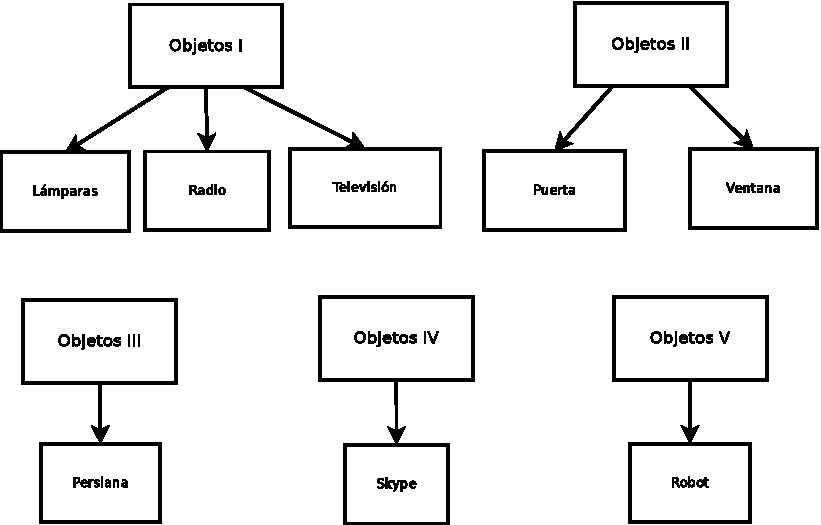
\includegraphics{Esquema_objetos}
  \caption{Clasificación de los objetos para la gramática (aquí también se pueden poner acrónimos como \acs{ETTS} y símbolos como \ac{xidet})}
  \label{fig:fig_clobj}
\end{figure}


\subsection{Definición y uso de acrónimos (aquí también se pueden poner acrónimos como \acs{ETTS})}
\label{sec:uso-de-acronimos}

El uso del paquete \texttt{glossaries} permite definir los acrónimos y el sistema automáticamente gestiona su inclusión completa la primera vez que se usa. Los acrónimos de ejemplo están en el fichero \texttt{acronyms/defacronymsgl.tex} (con opciones adicionales de configuración en \texttt{acronyms/acronymsgl.tex}).

Así, si nos referimos a \ac{ETTS} o bien a \ac{EMODB}, veremos como aparecen expandidas la primera vez. A partir de ahí, sólo se usará el acrónimo como puede verse al volver a hablar de \ac{ETTS} y \ac{EMODB}.

Tiene también soporte para resetear todos los acrónimos como si no estuvieran usados. Vuelvo a incluir el párrafo anterior tras un reset (que se hace con un \texttt{\textbackslash{}glsresetall[acronym]}):

\glsresetall[acronym]

El uso del paquete acronym permite definir los acrónimos y el sistema automáticamente gestiona su inclusión completa la primera vez que se usa. Así, si nos referimos a \ac{ETTS} o bien a \ac{EMODB}, veremos como aparecen expandidas de nuevo (como si fuera la primera vez que se usan). A partir de ahí, sólo se usará el acrónimo como puede verse al volver a hablar de \ac{ETTS} y \ac{EMODB}.

Y permite también forzar que se vuelva a citar completo aunque ya se haya utilizado (con el acrónimo entre paréntesis), como puede verse en \acl{ETTS} (equivalente a \glsdesc{ETTS} que vale para cualquier glosario), y también a usar forzosamente el acrónimo. Primero reseteamos de nuevo.

\glsresetall[acronym]

Y ahora forzamos el acrónimo: \acs{EMODB} (equivalente a \glsname{EMODB} que vale para cualquier glosario). También podemos forzar a que lo ponga todo, con \acf{EMODB}.


Podemos seguir definiendo entradas de acrónimos, referirnos a \ac{DBN} por primera vez, y las siguientes aparecerá como \ac{DBN}. Pongo ahora el resto de acrónimos \ac{SQ}, \ac{EIR}, \ac{SIR} y \ac{ES}. Finalmente los repito para que se vea el efecto: \ac{SQ}, \ac{EIR}, \ac{SIR} y \ac{ES}.

Y gestiona bien los plurales, ponemos el plural como \acp{SOC} la primera vez, y luego la segunda como \acp{SOC}. Y podemos volver al singular con \ac{SOC}.


\subsection{Definición y uso de símbolos (aquí también se pueden símbolos como \ac{xidet})}
\label{sec:simbolos}

Los símbolos definidos están incluidos en el fichero \texttt{symbols/defsymbolsgl.tex} (con configuración adicional en \texttt{symbols/symbolsgl.tex}) y en esta sección mostramos algunos ejemplos.

El \ac{angstrom} se usa en biología estructural, mientras que el \ac{ohm} se usa en electrónica. También podemos poner~\ac{xdet}. Y


\section{Ejemplos de inclusión de enlaces a vídeos y listado}
\label{sec:videolink}

En marzo de 2023 recibimos una pregunta sobre la posibilidad de incluir enlaces a vídeos en el documento, y que se generara automáticamente un listado similar al de tablas, figuras o algoritmos. El código para implementarlo está también en el fichero \texttt{cover/extralistings.tex} y puedes editarlo como te interese. Para usarlo, basta con que incluyas elementos similares a \videoLink{Introducción al Laboratorio de Circuitos Electrónicos (I)}{https://www.youtube.com/watch?v=U1P2ZP0f8KM} o \videoLink{Introducción al Laboratorio de Circuitos Electrónicos (V)}{https://www.youtube.com/watch?v=nPsxMqKRGx0}.

Lo importante no es tanto que sea un listado de vídeos, sino que muestra cómo se pueden integrar listados de elementos adicionales que sean a su vez enlaces y configurar la generación del índice para generar enlaces visitables desde el mismo índice (además de su indexación convencional).

%%% Local Variables:
%%% TeX-master: "../book"
%%% End:




%%%%%%%%%%%%%%%%%%%%%%%%%%%%%%%%%%%%%%%%%%%%%%%%%%%%%%%%%%%%%%%%%%%%%%%%%%%
%
% Generic template for TFC/TFM/TFG/Tesis
%
% $Id: estudioTeorico.tex,v 1.5 2015/06/05 00:05:19 macias Exp $
%
% By:
%  + Javier Macías-Guarasa.
%    Departamento de Electrónica
%    Universidad de Alcalá
%  + Roberto Barra-Chicote.
%    Departamento de Ingeniería Electrónica
%    Universidad Politécnica de Madrid
% 
% Based on original sources by Roberto Barra, Manuel Ocaña, Jesús Nuevo, Pedro Revenga, Fernando Herránz and Noelia Hernández. Thanks a lot to all of them, and to the many anonymous contributors found (thanks to google) that provided help in setting all this up.
%
% See also the additionalContributors.txt file to check the name of additional contributors to this work.
%
% If you think you can add pieces of relevant/useful examples, improvements, please contact us at (macias@depeca.uah.es)
%
% You can freely use this template and please contribute with comments or suggestions!!!
%
%%%%%%%%%%%%%%%%%%%%%%%%%%%%%%%%%%%%%%%%%%%%%%%%%%%%%%%%%%%%%%%%%%%%%%%%%%%

\chapter{Estudio teórico}
\label{cha:estudio-teorico}

\begin{FraseCelebre}
  \begin{Frase}
    Y así, del mucho leer y del poco dormir, se le secó el cerebro de manera que vino a perder el juicio\footnote{Tomado de ejemplos del proyecto \texis{}.}.
  \end{Frase}
  \begin{Fuente}
    Miguel de Cervantes Saavedra
  \end{Fuente}
\end{FraseCelebre}


\section{Introducción}
\label{sec:introduccion-teoria}

En este capítulo se cuenta tal y tal.

El capítulo se estructura en $n$ apartados\ldots


\section{Estado del Arte}
\label{sec:estadoarte}

En el estado del arte se enumeran los trabajos más relevantes de otros grupos de investigación. A continuación se muestra un ejemplo del uso de viñetas que nos proporciona \texttt{itemize}:

\begin{itemize}
  \item En el trabajo .....
  \item En el siguiente trabajo.....
\end{itemize}

O citas en un párrafo real: Sin embargo, hay entornos acústicos donde las tasas de error conseguidas son todavía demasiado altas. En concreto, las aplicaciones en las que la captura de la señal de habla se hace usando micrófonos alejados del locutor (típicamente para distancias superiores a un metro) muestran una fuerte sensibilidad a los problemas de reverberación, ruido aditivo y baja relación señal a ruido (\cite{gelbart02},\cite{kochkin02}). En estos entornos, se ha propuesto el uso de arrays de micrófonos como un método para mejorar la calidad del habla capturada \cite{seltzer03}\cite{herbordt05}.

Existen múltiples formas de insertar figuras en Latex. A continuación, se muestra un ejemplo del uso de \texttt{figure}. Como se puede ver en la Figura \ref{fig:fig1} también se pueden poner referencias a las figuras por medio de \texttt{ref} y la etiqueta \texttt{label} de la figura en particular.

\begin{figure}[h] %el especificador [h] indica que ponga la figura aqui si es posible
  \centering 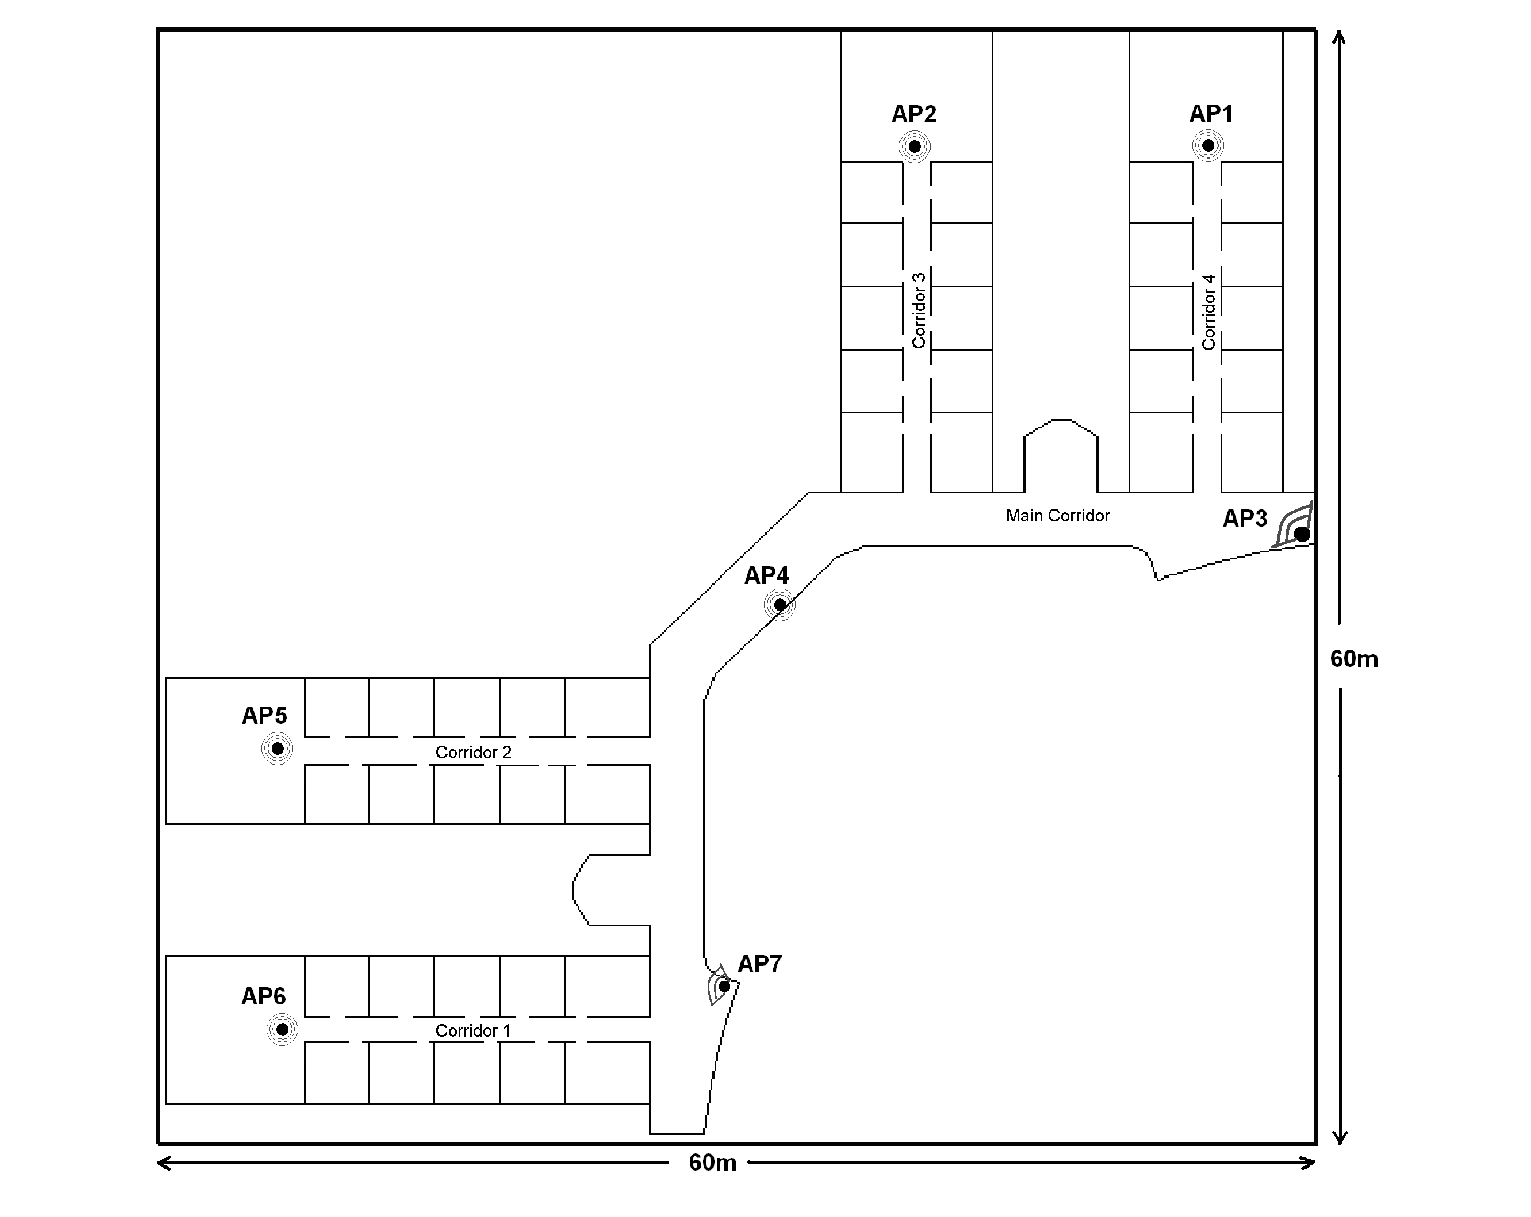
\includegraphics[width=4.7in]{Figure1}
  % where an .eps filename suffix will be assumed under latex, and a .pdf suffix will be assumed for pdflatex
  \caption{Departamento de Electrónica.}
  \label{fig:fig1}
\end{figure}

Y ahora un ejemplo en el que ponemos el \texttt{caption} en el lateral:

\begin{SCfigure}
  \centering 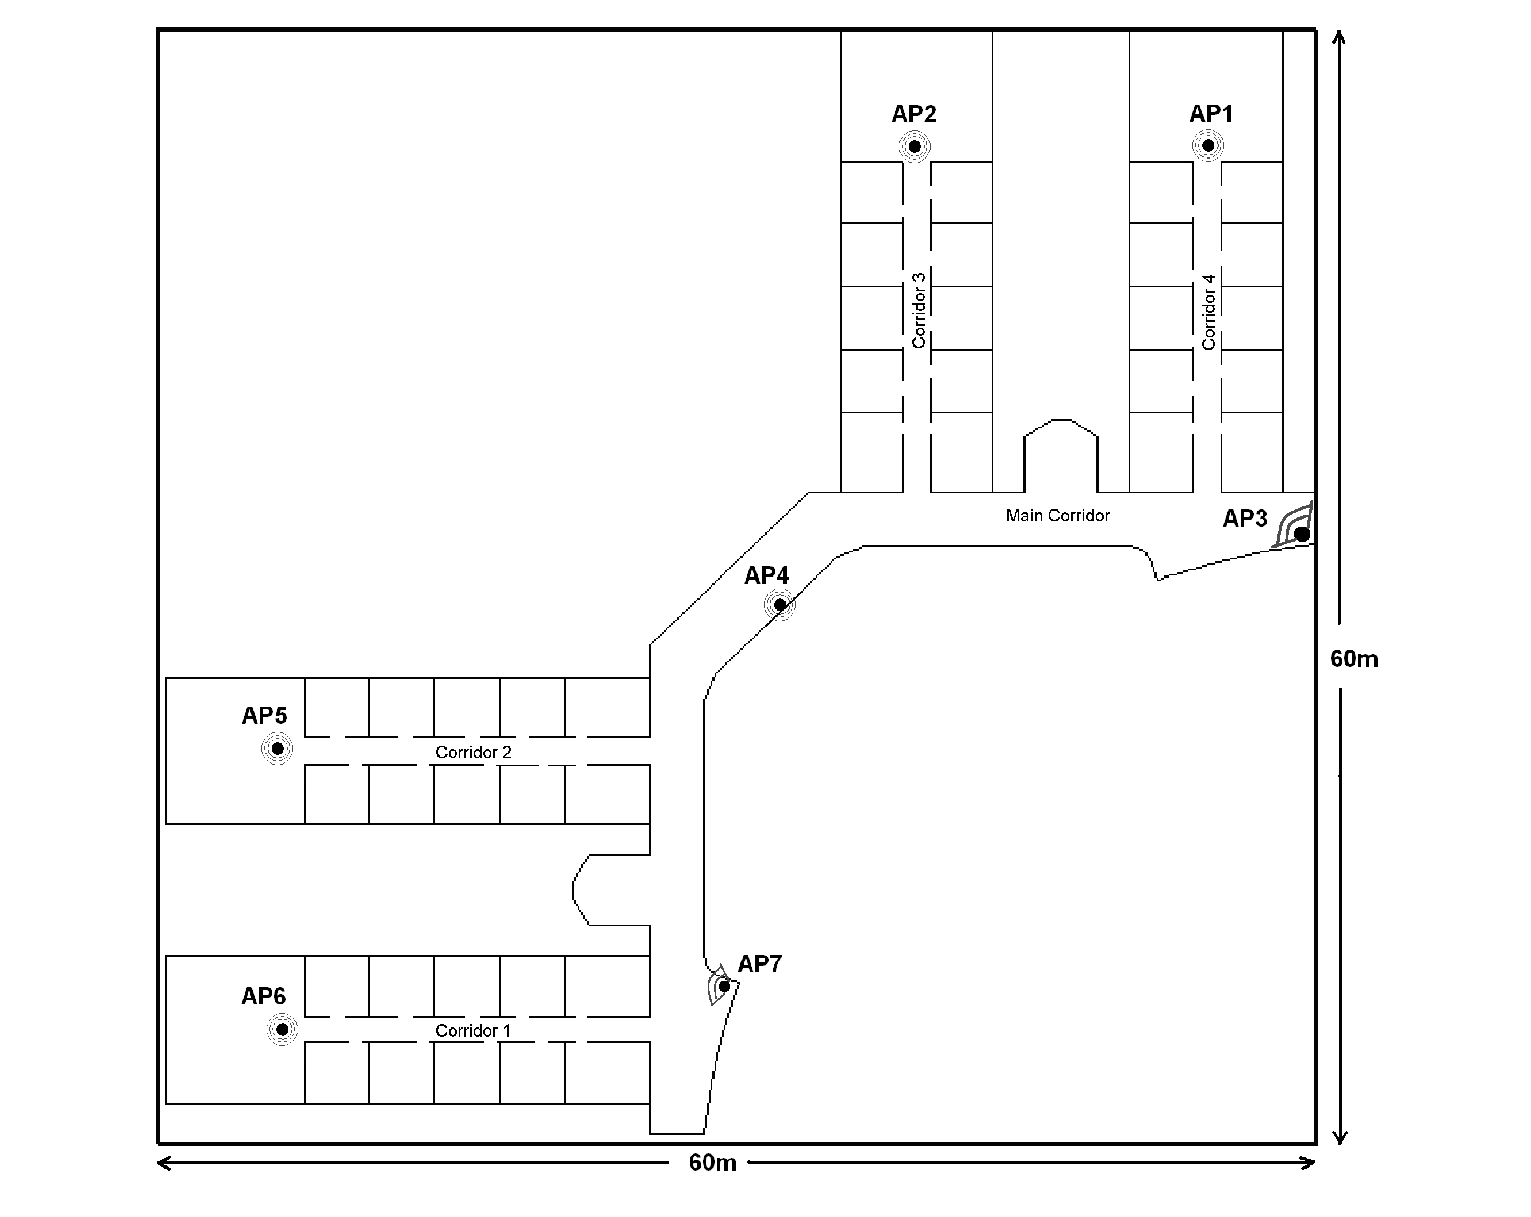
\includegraphics[width=0.5\textwidth]{Figure1}
  \caption{Departamento de Electrónica en el lateral.}
\end{SCfigure}



\section{Técnicas utilizadas}
\label{sec:tecnicas-utilizadas}

Aquí vamos a probar todos los niveles de sección disponibles, para evaluar la asignación de \texttt{tocdepth}...

Blah, blah, blah\ldots


\subsection{Subsección}
\label{sec:subseccion}


\subsubsection{Subsubsección}
\label{sec:subsubseccion}

\paragraph{Paragraph}
\label{sec:paragraph-1}


\subparagraph{Subparagraph}
\label{sec:subparagraph}



\section{Conclusiones}
\label{sec:conclusiones-teoria}

Blah, blah, blah\ldots

%%% Local Variables:
%%% TeX-master: "../book"
%%% End:


%%%%%%%%%%%%%%%%%%%%%%%%%%%%%%%%%%%%%%%%%%%%%%%%%%%%%%%%%%%%%%%%%%%%%%%%%%%
%
% Generic template for TFC/TFM/TFG/Tesis
%
% $Id: desarrollo.tex,v 1.1 2015/06/05 00:05:19 macias Exp $
%
% By:
%  + Javier Macías-Guarasa. 
%    Departamento de Electrónica
%    Universidad de Alcalá
%  + Roberto Barra-Chicote. 
%    Departamento de Ingeniería Electrónica
%    Universidad Politécnica de Madrid   
% 
% Based on original sources by Roberto Barra, Manuel Ocaña, Jesús Nuevo,
% Pedro Revenga, Fernando Herránz and Noelia Hernández. Thanks a lot to
% all of them, and to the many anonymous contributors found (thanks to
% google) that provided help in setting all this up.
%
% See also the additionalContributors.txt file to check the name of
% additional contributors to this work.
%
% If you think you can add pieces of relevant/useful examples,
% improvements, please contact us at (macias@depeca.uah.es)
%
% You can freely use this template and please contribute with
% comments or suggestions!!!
%
%%%%%%%%%%%%%%%%%%%%%%%%%%%%%%%%%%%%%%%%%%%%%%%%%%%%%%%%%%%%%%%%%%%%%%%%%%%

\chapter{Desarrollo}
\label{cha:development}


\begin{FraseCelebre}
  \begin{Frase}
    A fuerza de construir bien, se llega a buen
    arquitecto\footnote{Tomado de ejemplos del proyecto \texis{}.}.
  \end{Frase}
  \begin{Fuente}
    Aristóteles
  \end{Fuente}
\end{FraseCelebre}



\section{Introducción}
\label{sec:development-introduction}

Blah, blah, blah.

La estructura de este capítulo es\ldots


\section{Sección 1 del capítulo de desarrollo}
\label{sec:development-1}

Blah, blah, blah.


\subsection{Subsección 1.1 del capítulo de desarrollo}
\label{sec:development-11}

Blah, blah, blah.


\subsection{Subsección 1.2 del capítulo de desarrollo}
\label{sec:development-12}

Blah, blah, blah.



\section{Sección 2 del capítulo de desarrollo}
\label{sec:development-2}

Blah, blah, blah.




\section{Conclusiones}
\label{sec:development-conclusions}

Blah, blah, blah.



%%% Local Variables:
%%% TeX-master: "../book"
%%% End:


%%%%%%%%%%%%%%%%%%%%%%%%%%%%%%%%%%%%%%%%%%%%%%%%%%%%%%%%%%%%%%%%%%%%%%%%%%%
%
% Generic template for TFC/TFM/TFG/Tesis
%
% $Id: resultados.tex,v 1.1 2015/06/05 00:05:20 macias Exp $
%
% By:
%  + Javier Macías-Guarasa. 
%    Departamento de Electrónica
%    Universidad de Alcalá
%  + Roberto Barra-Chicote. 
%    Departamento de Ingeniería Electrónica
%    Universidad Politécnica de Madrid   
% 
% Based on original sources by Roberto Barra, Manuel Ocaña, Jesús Nuevo,
% Pedro Revenga, Fernando Herránz and Noelia Hernández. Thanks a lot to
% all of them, and to the many anonymous contributors found (thanks to
% google) that provided help in setting all this up.
%
% See also the additionalContributors.txt file to check the name of
% additional contributors to this work.
%
% If you think you can add pieces of relevant/useful examples,
% improvements, please contact us at (macias@depeca.uah.es)
%
% Copyleft 2013
%
%%%%%%%%%%%%%%%%%%%%%%%%%%%%%%%%%%%%%%%%%%%%%%%%%%%%%%%%%%%%%%%%%%%%%%%%%%%

\chapter{Resultados}
\label{cha:resultados}


\begin{FraseCelebre}
  \begin{Frase}
    % Si quieres ser leído más de una vez, no vaciles en borrar a menudo.
    Rem tene, verba sequentur (Si dominas el tema, las palabras vendrán
    solas)\footnote{Tomado de ejemplos del proyecto \texis{}.}.
  \end{Frase}
  \begin{Fuente}
    % Horacio
    Catón el Viejo
  \end{Fuente}
\end{FraseCelebre}

\section{Introducción}
\label{sec:results-introduction}

Blah, blah, blah.

La estructura de este capítulo es\ldots


\section{Sección 1 del capítulo de resultados}
\label{sec:results-1}

Blah, blah, blah.


\subsection{Subsección 1.1 del capítulo de resultados}
\label{sec:results-11}

Blah, blah, blah.


\subsection{Subsección 1.2 del capítulo de resultados}
\label{sec:results-12}

Blah, blah, blah.




\section{Sección 2 del capítulo de resultados}
\label{sec:results-2}

Blah, blah, blah.




\section{Conclusiones}
\label{sec:results-conclusions}

Blah, blah, blah.


%%% Local Variables:
%%% TeX-master: "../book"
%%% End:


%%%%%%%%%%%%%%%%%%%%%%%%%%%%%%%%%%%%%%%%%%%%%%%%%%%%%%%%%%%%%%%%%%%%%%%%%%%
%
% Generic template for TFC/TFM/TFG/Tesis
%
% By:
%  + Javier Macías-Guarasa.
%    Departamento de Electrónica
%    Universidad de Alcalá
%  + Roberto Barra-Chicote.
%    Departamento de Ingeniería Electrónica
%    Universidad Politécnica de Madrid
%
% By: + Javier Macías-Guarasa. Departamento de Electrónica Universidad de Alcalá + Roberto Barra-Chicote. Departamento de Ingeniería Electrónica Universidad Politécnica de Madrid
% 
% Based on original sources by Roberto Barra, Manuel Ocaña, Jesús Nuevo, Pedro Revenga, Fernando Herránz and Noelia Hernández. Thanks a lot to all of them, and to the many anonymous contributors found (thanks to google) that provided help in setting all this up.
%
% See also the additionalContributors.txt file to check the name of additional contributors to this work.
%
% If you think you can add pieces of relevant/useful examples, improvements, please contact us at (macias@depeca.uah.es)
%
% You can freely use this template and please contribute with comments or suggestions!!!
%
%%%%%%%%%%%%%%%%%%%%%%%%%%%%%%%%%%%%%%%%%%%%%%%%%%%%%%%%%%%%%%%%%%%%%%%%%%%

\chapter{Conclusiones y líneas futuras}
\label{cha:concl-y-line}

En este apartado se resumen las conclusiones obtenidas y se proponen futuras líneas de investigación que se deriven del trabajo.

La estructura del capítulo es...


\section{Conclusiones}
\label{sec:conclusiones}

Para añadir una referencia a un autor, se puede utilizar el paquete \texttt{cite}. En el trabajo \cite{armani03}, se muestra un trabajo...

Y podemos usar de nuevo algún acrónimo, como por ejemplo \ac{TDPSOLA}, o uno ya referenciado como \ac{ANN} que cambia cuando lo usas una segunda vez \ac{ANN}.

Veamos finalmente si funciona una cita inline... al paper de Leticia \fullcite{monasterio2022}... (esto substituye la funcionalidad de bibentry...).


\section{Líneas futuras}
\label{sec:lineas-futuras}

Pues eso.


%%% Local Variables:
%%% TeX-master: "../book"
%%% End:




% Optional in PFCs
%%%%%%%%%%%%%%%%%%%%%%%%%%%%%%%%%%%%%%%%%%%%%%%%%%%%%%%%%%%%%%%%%%%%%%%%%%%%
%
% Generic template for TFC/TFM/TFG/Tesis
%
% $Id: pliego-ejemplo.tex,v 1.2 2015/06/05 00:10:36 macias Exp $
%
% By:
%  + Javier Macías-Guarasa. 
%    Departamento de Electrónica
%    Universidad de Alcalá
%  + Roberto Barra-Chicote. 
%    Departamento de Ingeniería Electrónica
%    Universidad Politécnica de Madrid   
% 
% Based on original sources by Roberto Barra, Manuel Ocaña, Jesús Nuevo,
% Pedro Revenga, Fernando Herránz and Noelia Hernández. Thanks a lot to
% all of them, and to the many anonymous contributors found (thanks to
% google) that provided help in setting all this up.
%
% See also the additionalContributors.txt file to check the name of
% additional contributors to this work.
%
% If you think you can add pieces of relevant/useful examples,
% improvements, please contact us at (macias@depeca.uah.es)
%
% You can freely use this template and please contribute with
% comments or suggestions!!!
%
%%%%%%%%%%%%%%%%%%%%%%%%%%%%%%%%%%%%%%%%%%%%%%%%%%%%%%%%%%%%%%%%%%%%%%%%%%%

\chapter{Pliego de condiciones}
\label{cha:pliego-de-condiciones}

\section{Introducción}

En este apartado se evaluaran las condiciones para poner en marcha el software que se ha especificado en los apartados anteriores. Cabe resaltar el carácter de este proyecto, en el que se ha diseñado una colección de funciones que facilitan al programador la correcta adquisición de datos sonoros, y por lo tanto no aplican las condiciones técnicas o ambientales que pudieran afectarle, ya que las impone los requerimientos las aplicaciones que en un futuro se le quiera dar a este proyecto.

Solamente afectan las condiciones de configuración hardware o software donde se quiera aplicar el programa informático.

\section{Requisitos de hardware}

\subsection{Requisitos mínimos}
\begin{itemize}
  \item Utilización de un PC de 32 bits de escritorio con tarjeta de sonido.
  \item Un mínimo de 384 MB de memoria RAM.
  \item Al menos 100 MB de memoria libre en disco duro.
\end{itemize}

\subsection{Requisitos de hardware recomendados}
Estos requisitos son necesarios para implementar algoritmos de localización basados en onda sonora.
\begin{itemize}
  \item CPU de 64 bits con 4 Cores o más.
  \item Sistema de adquisición con 8 canales o más.
  \item Utilización de al menos 4 Gb de memoria RAM.
\end{itemize}

\section{Condiciones hardware}

El sistema de adquisición que se propone hace uso de 4 hilos independientes en la adquisición en tiempo real. Es por esta razón que se recomienda sistemas multiprocesador, que permitan realizar las tareas de cada hilo de manera independiente.

Se precisa de un sistema de adquisición de audio profesional para la adquisición del audio proveniente de cada micrófono para ejecutar el algoritmo de localización. Además por esta razón y porque se van a generar gran cantidad de datos a procesar en la memoria RAM del equipo, es necesaria la utilización de un volumen importante de memoria RAM, se recomienda que la cifra de partida sean 4 Gb que es la cifra máxima que un sistema operativo de 32 bits basado en Linux puede direccionar.

Se recomienda tener 100 MB de disco duro libre para poder hacer grabaciones de corta duración. Es altamente recomendable disponer de 10 GB libres si se van a realizar grabaciones multicanal y de larga duración.
 
\section{Requisitos de software}

\subsection{Requisitos mínimos}
\begin{itemize}
  \item Utilización de un sistema operativo Ubuntu 12.04.
  \item Librería \texttt{Rtaudio}.
  \item Librería \texttt{SNDFile}.
  \item Para el desarrollo del algoritmo de localización se deben utilizar las librerías propias del grupo GEINTRA.
\end{itemize}

\subsection{Requisitos de software recomendados}
\begin{itemize}
  \item Utilización de un sistema operativo de 64 bits, Ubuntu 12.04 o superior.
\end{itemize}

\section{Condiciones software}

En este apartado software se recomienda utilizar el sistema operativo Ubuntu 12.04 al ser LTS, y proporcionar la compatibilidad con las nuevas librerías Qt para realizar profiling mediante KCachegrind.

En el caso de disponer un sistema hardware con una memoria RAM superior a 4 GB es necesario utilizar, una verisón de Ubuntu de 64 bits para poder direccionarla. Es muy recomendable esta opción para poder adquirir y procesar sonido multicanal.

\newpage
\section{Condiciones generales}

La utilización de esta librería supone la posibilidad de ejecutar cualquier programa de procesamiento sobre ella que tenga en cuenta las siguientes condiciones:

\begin{itemize}
  \item El ancho de banda de las señales acústicas está condicionado por el rango que permita la tarjeta de adquisición a utilizar, por lo general cumple aproximadamente la del espectro del oído humano, de 20 a 20000 Hz.
  \item El número de canales a utilizar lo limita la tarjeta de adquisición, la librería está preparada para adquirir, sea cual sea el rango multicanal.
  \item Ante cualquier uso de esta librería deberá tenerse en cuenta el reconocimiento (BY), que no es comercial (NC), y que las obras derivadas se compartan de igual manera (SA).

\end{itemize}

%%% Local Variables:
%%% TeX-master: "../book"
%%% End:


% Optional in PFCs, compulsory in TFGs
%%%%%%%%%%%%%%%%%%%%%%%%%%%%%%%%%%%%%%%%%%%%%%%%%%%%%%%%%%%%%%%%%%%%%%%%%%%%
%
% Generic template for TFC/TFM/TFG/Tesis
%
% $Id: presupuesto.tex,v 1.5 2015/06/05 00:10:36 macias Exp $
%
% By:
%  + Javier Macías-Guarasa. 
%    Departamento de Electrónica
%    Universidad de Alcalá
%  + Roberto Barra-Chicote. 
%    Departamento de Ingeniería Electrónica
%    Universidad Politécnica de Madrid   
% 
% Based on original sources by Roberto Barra, Manuel Ocaña, Jesús Nuevo,
% Pedro Revenga, Fernando Herránz and Noelia Hernández. Thanks a lot to
% all of them, and to the many anonymous contributors found (thanks to
% google) that provided help in setting all this up.
%
% See also the additionalContributors.txt file to check the name of
% additional contributors to this work.
%
% If you think you can add pieces of relevant/useful examples,
% improvements, please contact us at (macias@depeca.uah.es)
%
% You can freely use this template and please contribute with
% comments or suggestions!!!
%
%%%%%%%%%%%%%%%%%%%%%%%%%%%%%%%%%%%%%%%%%%%%%%%%%%%%%%%%%%%%%%%%%%%%%%%%%%%

\chapter{Presupuesto}
\label{cha:presupuesto}


En este capítulo se incluye una estimación del coste total para la realización del proyecto. En las siguientes secciones los costes son divididos en función de su origen, exponiendo el subtotal en cada uno de los apartados y al final se añade el total de estas cifras.

\section{Recursos Hardware}
\label{sec:presupuesto-hardware}

Se ha necesitado gran cantidad de recursos hardware para construir la plataforma y que funcione correctamente. Dichos recursos son enumerados en el siguiente listado.

\begin{itemize}
    \item Chasis.
    \item Ruedas.
    \item Baterías.
    \item Motores y encoders.
    \item Piezas 3D.
    \item Material básico de electrónica (resistencias, condensadores, LEDs, etc).
    \item Drivers para motores.
    \item Tarjetas microcontroladoras LPC2129.
    \item Joystick analógico inductivo.
\end{itemize}

El precio y las unidades son incluidos en la tabla \ref{tab:recursos_hardware} junto con el total de los recursos hardware.

\begin{table}[H]
\centering
\begin{tabular}{|c|c|c|c|}
\hline
Concepto                & Precio por Unidad & Cantidad & Subtotal \\ \hline
Chasis                  & 50,00 \euro               & 1        & 50,00 \euro        \\ \hline
Ruedas                  & 10,00 \euro                & 4        & 40,00 \euro       \\ \hline
Baterías                & 40,00 \euro                & 2        & 80,00 \euro       \\ \hline
Motor y encoder         & 20,00 \euro                & 2        & 40,00 \euro       \\ \hline
Piezas 3D               & 15,00 \euro                & 1        & 15,00 \euro       \\ \hline
Material de electrónica & 60,00 \euro                & 1        & 60,00 \euro       \\ \hline
Drivers                 & 30,00 \euro                & 2        & 60,00 \euro       \\ \hline
LPC2129                 & 50,00 \euro                & 2        & 100,00 \euro      \\ \hline
Joystick                & 110,00 \euro               & 1        & 110,00 \euro      \\ \hline
\multicolumn{3}{|c|}{TOTAL}                            & 555,00 \euro     \\ \hline
\end{tabular}
\caption{Recursos hardware usados}
\label{tab:recursos_hardware}
\end{table}

\section{Recursos de desarrollo y pruebas}
\label{sec:presupuesto-software}

Para llevar a cabo este trabajo es necesario el uso de determinado software, que involucra la programación de los nodos, el diseño electrónico de los mismos, la simulación de la plataforma, etc. A continuación se incluye un listado de los programas usados para dichas tareas. El precio se ha calculado en función de la vida útil del recurso (2 años) y el tiempo utilizado (2 meses).

\begin{itemize}
    \item Matlab para diseño de controlador PI, representación de gráficas y pruebas.
    \item OrCAD para diseño de circuitos electrónicos.
    \item $\mu$Vision de Keil para programación de microcontroladores.
    \item FreeCAD. Este programa es gratuito y se ha usado para diseño de piezas 3D y modelado de la plataforma.
\end{itemize}

En la tabla \ref{tab:recursos_software} se incluyen dichos programas con sus respectivos costes de licencia.

\begin{table}[H]
\centering
\begin{tabular}{|c|c|c|c|}
\hline
Concepto    & Precio por Unidad & Coeficiente & Subtotal \\ \hline
Matlab      & 200,00 \euro                 & 0,0833        & 16,66 \euro        \\ \hline
$\mu$Vision & 400,00 \euro                 & 0,0833        & 33,32 \euro        \\ \hline
FreeCAD       & 0,00 \euro                 & 0,0833        & 0,00 \euro       \\ \hline
OrCAD     & 125,00 \euro                 & 0,0833        & 10,41 \euro        \\ \hline
Portatil Lenovo Yoga     & 700,00 \euro                 & 0,0833        & 58,31 \euro        \\ \hline
\multicolumn{3}{|c|}{TOTAL}                & 118,70 \euro        \\ \hline
\end{tabular}
\caption{Recursos de desarrollo y pruebas}
\label{tab:recursos_software}
\end{table}

\section{Recursos Humanos}
\label{sec:presupuesto-mano}

El coste proveniente a los recursos humanos del trabajo provienen de un ingeniero que desarrolla el trabajo completo. A continuación se incluyen dichos costes.

\begin{table}[H]
\centering
\begin{tabular}{|c|c|c|c|}
\hline
Concepto  & Precio por hora & Cantidad de horas & Subtotal \\ \hline
Ingeniero & 50,00 \euro              & 500                 & 25000,00 \euro       \\ \hline
\multicolumn{3}{|c|}{TOTAL}                     & 25000,00 \euro        \\ \hline
\end{tabular}
\caption{Recursos humanos}
\label{tab:recursos_humanos}
\end{table}

\section{Presupuesto de ejecución material}
\label{sec:presupuesto-material}

El presupuesto de ejecución material es la suma de los recursos hardware, software y humanos necesarios para llevar a cabo el trabajo.

\begin{table}[H]
\centering
\begin{tabular}{|c|c|}
\hline
Concepto           & Subtotal \\ \hline
Recursos hardware  & 555,00 \euro        \\ \hline
Recursos software  & 118,70 \euro        \\ \hline
Coste mano de obra & 25000,00 \euro        \\ \hline
TOTAL              & 25673,70 \euro        \\ \hline
\end{tabular}
\caption{Presupuesto de ejecución material}
\label{tab:ejec_material}
\end{table}

\section{Importe de la ejecución por contrata}
\label{sec:presupuesto-ejecucion}

Los costes de la ejecución por contrata deben incluir los gastos derivados del uso de las instalaciones donde se ha llevado a cabo el trabajo, las cargas fiscales, los gastos financiero, las tasas administrativas y las obligaciones de control del proyecto.

Dicho gasto se asume estableciendo un recargo sobre el coste del importe del presupuesto de ejecución material. Dicho recargo equivale al 22\% de dicho importe

\begin{table}[H]
\centering
\begin{tabular}{|c|c|}
\hline
Concepto                                      & Subtotal \\ \hline
22\% del coste total de ejecución de material & 5648,21 \euro       \\ \hline
\end{tabular}
\caption{Importe de ejecución por contrata}
\label{tab:ejec_contrata}
\end{table}


\section{Honorarios facultativos}
\label{sec:presupuesto-facultativos}

Se fija en este proyecto un porcentaje del 7\% sobre el coste total de ejecución por contrata.

\begin{table}[H]
\centering
\begin{tabular}{|c|c|}
\hline
Concepto                                & Subtotal \\ \hline
7\% del coste de ejecución por contrata & 395,38 \euro        \\ \hline
\end{tabular}
\caption{Importe de los honorarios facultativos}
\label{tab:honorarios}
\end{table}

\section{Presupuesto Total}
\label{sec:presupuesto-total}

A continuación, en la tabla \ref{tab:presupuesto_total} se realiza la suma de todos los conceptos del presupuesto tenidos en cuenta en los anteriores apartados.

\begin{table}[H]
\centering
\begin{tabular}{|c|c|}
\hline
Concepto Precio                    & Subtotal \\ \hline
Presupuesto de ejecución material  & 25673,70 \euro        \\ \hline
Importe de la ejecución contratada & 5648,21 \euro        \\ \hline
Horarios facultativos              & 395,38 \euro        \\ \hline
TOTAL (sin IVA)                    & 31717,29 \euro        \\ \hline
IVA (22 \%)                        & 6977,80\euro        \\ \hline
TOTAL                              & 38695,10 \euro        \\ \hline
\end{tabular}
\caption{Importe del presupuesto total del proyecto}
\label{tab:presupuesto_total}
\end{table}

%%% Local Variables:
%%% TeX-master: "../book"
%%% End:


%
% END Normal chapters. Edit/modify all within this section
%%%%%%%%%%%%%%%%%%%%%%%%%%%%%%%%%%%%%%%%%%%%%%%%%%%%%%%%%%%%%%%%%%%%%%%%%%%
%%%%%%%%%%%%%%%%%%%%%%%%%%%%%%%%%%%%%%%%%%%%%%%%%%%%%%%%%%%%%%%%%%%%%%%%%%%
%%%%%%%%%%%%%%%%%%%%%%%%%%%%%%%%%%%%%%%%%%%%%%%%%%%%%%%%%%%%%%%%%%%%%%%%%%%
%%%%%%%%%%%%%%%%%%%%%%%%%%%%%%%%%%%%%%%%%%%%%%%%%%%%%%%%%%%%%%%%%%%%%%%%%%%
%%%%%%%%%%%%%%%%%%%%%%%%%%%%%%%%%%%%%%%%%%%%%%%%%%%%%%%%%%%%%%%%%%%%%%%%%%%
%%%%%%%%%%%%%%%%%%%%%%%%%%%%%%%%%%%%%%%%%%%%%%%%%%%%%%%%%%%%%%%%%%%%%%%%%%%
%%%%%%%%%%%%%%%%%%%%%%%%%%%%%%%%%%%%%%%%%%%%%%%%%%%%%%%%%%%%%%%%%%%%%%%%%%%


%%%%%%%%%%%%%%%%%%%%%%%%%%%%%%%%%%%%%%%%%%%%%%%%%%%%%%%%%%%%%%%%%%%%%%%%%%%
% Bibliography
%%%%%%%%%%%%%%%%%%%%%%%%%%%%%%%%%%%%%%%%%%%%%%%%%%%%%%%%%%%%%%%%%%%%%%%%%%%
%%%%%%%%%%%%%%%%%%%%%%%%%%%%%%%%%%%%%%%%%%%%%%%%%%%%%%%%%%%%%%%%%%%%%%%%%%%
%
% Generic template for TFC/TFM/TFG/Tesis
%
% $Id: bibliography.tex,v 1.9 2015/06/05 00:10:32 macias Exp $
%
% By:
%  + Javier Macías-Guarasa. 
%    Departamento de Electrónica
%    Universidad de Alcalá
%  + Roberto Barra-Chicote. 
%    Departamento de Ingeniería Electrónica
%    Universidad Politécnica de Madrid   
% 
% Based on original sources by Roberto Barra, Manuel Ocaña, Jesús Nuevo,
% Pedro Revenga, Fernando Herranz and Noelia Hernández. Thanks a lot to
% all of them, and to the many anonymous contributors found (thanks to
% google) that provided help in setting all this up.
%
% See also the additionalContributors.txt file to check the name of
% additional contributors to this work.
%
% If you think you can add pieces of relevant/useful examples,
% improvements, please contact us at (macias@depeca.uah.es)
%
% You can freely use this template and please contribute with
% comments or suggestions!!!
%
%%%%%%%%%%%%%%%%%%%%%%%%%%%%%%%%%%%%%%%%%%%%%%%%%%%%%%%%%%%%%%%%%%%%%%%%%%%

% IMPORTANT: YOU DON'T HAVE TO EDIT THIS FILE, JUST EDIT THE bibliofiles.tex file
% IMPORTANT: YOU DON'T HAVE TO EDIT THIS FILE, JUST EDIT THE bibliofiles.tex file
% IMPORTANT: YOU DON'T HAVE TO EDIT THIS FILE, JUST EDIT THE bibliofiles.tex file
% IMPORTANT: YOU DON'T HAVE TO EDIT THIS FILE, JUST EDIT THE bibliofiles.tex file
% IMPORTANT: YOU DON'T HAVE TO EDIT THIS FILE, JUST EDIT THE bibliofiles.tex file
% IMPORTANT: YOU DON'T HAVE TO EDIT THIS FILE, JUST EDIT THE bibliofiles.tex file
% IMPORTANT: YOU DON'T HAVE TO EDIT THIS FILE, JUST EDIT THE bibliofiles.tex file
% IMPORTANT: YOU DON'T HAVE TO EDIT THIS FILE, JUST EDIT THE bibliofiles.tex file
% IMPORTANT: YOU DON'T HAVE TO EDIT THIS FILE, JUST EDIT THE bibliofiles.tex file
% IMPORTANT: YOU DON'T HAVE TO EDIT THIS FILE, JUST EDIT THE bibliofiles.tex file
% IMPORTANT: YOU DON'T HAVE TO EDIT THIS FILE, JUST EDIT THE bibliofiles.tex file
% IMPORTANT: YOU DON'T HAVE TO EDIT THIS FILE, JUST EDIT THE bibliofiles.tex file
% IMPORTANT: YOU DON'T HAVE TO EDIT THIS FILE, JUST EDIT THE bibliofiles.tex file
% IMPORTANT: YOU DON'T HAVE TO EDIT THIS FILE, JUST EDIT THE bibliofiles.tex file
% IMPORTANT: YOU DON'T HAVE TO EDIT THIS FILE, JUST EDIT THE bibliofiles.tex file
% IMPORTANT: YOU DON'T HAVE TO EDIT THIS FILE, JUST EDIT THE bibliofiles.tex file
% IMPORTANT: YOU DON'T HAVE TO EDIT THIS FILE, JUST EDIT THE bibliofiles.tex file
% IMPORTANT: YOU DON'T HAVE TO EDIT THIS FILE, JUST EDIT THE bibliofiles.tex file
% IMPORTANT: YOU DON'T HAVE TO EDIT THIS FILE, JUST EDIT THE bibliofiles.tex file
% IMPORTANT: YOU DON'T HAVE TO EDIT THIS FILE, JUST EDIT THE bibliofiles.tex file
% IMPORTANT: YOU DON'T HAVE TO EDIT THIS FILE, JUST EDIT THE bibliofiles.tex file


\ifthenelse{\equal{\bibliosystem}{biblatex}}
{
  % Use biblatex instead of bibtex

  %% Wen changing to biblatex, we could not define here the bibliography files, so that
  %% You need to edit the bibliofiles.tex file to do so

  %% % Now add all bib files to be processed
  %% \addbibresource{\myreferencespath\mybibfileOne}
  %% % \addbibresource{\myreferencespath\mybibfileTwo}
  %% % ...
  %% % \addbibresource{\myreferencespath\mybibfileN}

  \printbibliography[heading=bibintoc]


}
{
  % Use bibtex

  %\bibliographystyle{plainnat}
  %\bibliographystyle{dinat}
  %\bibliographystyle{unsrt}
  \bibliographystyle{IEEEtran}

  % The following is overly complicated because I was not able to do so in
  % another way. The problem is the bibliography command being "called"
  % from both the root and anteproyecto directories...
  %
  %% Here define as many bibfiles as needed
%%
%% It is compulsory that they are named as \mybibfileOne
%% \mybibfileTwo, \mybibfileThree, ... \mybibfileTen
%%
%% If you need more than ten, you will have to edit
%% Config/preamble.tex and Book/biblio/bibliography.tex
%% to support this adition
%%
%% The file names may change at your will, but they must
%% be in the Book/biblio directory

\newcommand{\mybibfileOne}{biblio/biblio.bib}


  \newcommand{\mybibfiles}{}
  \ifdef{\mybibfileOne}
  {
  \let\oldmybibfiles\mybibfiles
  \renewcommand{\mybibfiles}{\myreferencespath\mybibfileOne}
  }
  {
  \errorYOUmustDEFINEatLEASTmybibfileOneInbibliofilesDOTtex
  }
  \ifdef{\mybibfileTwo}
  {
  \let\oldmybibfiles\mybibfiles
  \renewcommand{\mybibfiles}{\oldmybibfiles,\myreferencespath\mybibfileTwo}
  }
  {
  }
  \ifdef{\mybibfileThree}
  {
  \let\oldmybibfiles\mybibfiles
  \renewcommand{\mybibfiles}{\oldmybibfiles,\myreferencespath\mybibfileThree}
  }
  {
  }

  \ifdef{\mybibfileFour}
  {
  \let\oldmybibfiles\mybibfiles
  \renewcommand{\mybibfiles}{\oldmybibfiles,\myreferencespath\mybibfileFour}
  }
  {
  }
  \ifdef{\mybibfileSix}
  {
  \let\oldmybibfiles\mybibfiles
  \renewcommand{\mybibfiles}{\oldmybibfiles,\myreferencespath\mybibfileSix}
  }
  {
  }

  \ifdef{\mybibfileSeven}
  {
  \let\oldmybibfiles\mybibfiles
  \renewcommand{\mybibfiles}{\oldmybibfiles,\myreferencespath\mybibfileSeven}
  }
  {
  }

  \ifdef{\mybibfileEight}
  {
  \let\oldmybibfiles\mybibfiles
  \renewcommand{\mybibfiles}{\oldmybibfiles,\myreferencespath\mybibfileEight}
  }
  {
  }

  \ifdef{\mybibfileNine}
  {
  \let\oldmybibfiles\mybibfiles
  \renewcommand{\mybibfiles}{\oldmybibfiles,\myreferencespath\mybibfileNine}
  }
  {
  }

  \ifdef{\mybibfileTen}
  {
  \let\oldmybibfiles\mybibfiles
  \renewcommand{\mybibfiles}{\oldmybibfiles,\myreferencespath\mybibfileTen}
  }
  {
  }

  \ifdef{\mybibfileEleven}
  {
    \let\oldmybibfiles\mybibfiles
    \renewcommand{\mybibfiles}{\oldmybibfiles,\myreferencespath\mybibfileEleven}
  }
  {
  }

  \ifdef{\mybibfileTwelve}
  {
    \let\oldmybibfiles\mybibfiles
    \renewcommand{\mybibfiles}{\oldmybibfiles,\myreferencespath\mybibfileTwelve}
  }
  {
  }

  \ifdef{\mybibfileThirteen}
  {
    \let\oldmybibfiles\mybibfiles
    \renewcommand{\mybibfiles}{\oldmybibfiles,\myreferencespath\mybibfileThirteen}
  }
  {
  }

  \ifdef{\mybibfileFourteen}
  {
    \let\oldmybibfiles\mybibfiles
    \renewcommand{\mybibfiles}{\oldmybibfiles,\myreferencespath\mybibfileFourteen}
  }
  {
  }

  \ifdef{\mybibfileFifteen}
  {
    \let\oldmybibfiles\mybibfiles
    \renewcommand{\mybibfiles}{\oldmybibfiles,\myreferencespath\mybibfileFifteen}
  }
  {
  }

  \ifdef{\mybibfileSixteen}
  {
    \let\oldmybibfiles\mybibfiles
    \renewcommand{\mybibfiles}{\oldmybibfiles,\myreferencespath\mybibfileSixteen}
  }
  {
  }

  \ifdef{\mybibfileSeventeen}
  {
    \let\oldmybibfiles\mybibfiles
    \renewcommand{\mybibfiles}{\oldmybibfiles,\myreferencespath\mybibfileSeventeen}
  }
  {
  }

  \ifdef{\mybibfileEighteen}
  {
    \let\oldmybibfiles\mybibfiles
    \renewcommand{\mybibfiles}{\oldmybibfiles,\myreferencespath\mybibfileEighteen}
  }
  {
  }

  \ifdef{\mybibfileNineteen}
  {
    \let\oldmybibfiles\mybibfiles
    \renewcommand{\mybibfiles}{\oldmybibfiles,\myreferencespath\mybibfileNineteen}
  }
  {
  }

  \ifdef{\mybibfileTwenty}
  {
    \let\oldmybibfiles\mybibfiles
    \renewcommand{\mybibfiles}{\oldmybibfiles,\myreferencespath\mybibfileTwenty}
  }
  {
  }

  \ifdef{\mybibfileTwentyone}
  {
    \let\oldmybibfiles\mybibfiles
    \renewcommand{\mybibfiles}{\oldmybibfiles,\myreferencespath\mybibfileTwentyone}
  }
  {
  }

  \ifdef{\mybibfileTwentytwo}
  {
    \let\oldmybibfiles\mybibfiles
    \renewcommand{\mybibfiles}{\oldmybibfiles,\myreferencespath\mybibfileTwentytwo}
  }
  {
  }

  \ifdef{\mybibfileTwentythree}
  {
    \let\oldmybibfiles\mybibfiles
    \renewcommand{\mybibfiles}{\oldmybibfiles,\myreferencespath\mybibfileTwentythree}
  }
  {
  }

  \ifdef{\mybibfileTwentyfour}
  {
    \let\oldmybibfiles\mybibfiles
    \renewcommand{\mybibfiles}{\oldmybibfiles,\myreferencespath\mybibfileTwentyfour}
  }
  {
  }

  \ifdef{\mybibfileTwentyfive}
  {
    \let\oldmybibfiles\mybibfiles
    \renewcommand{\mybibfiles}{\oldmybibfiles,\myreferencespath\mybibfileTwentyfive}
  }
  {
  }

  % Do not touch this
  % The commands around the \bibliography{} command should be included if using bibtex, but
  % according to Gonzalo Corral's PR on July 2022, they break compilation in overleaf. I think
  % this should not happen if the bib files are in iso-8859-1 when using bibtex instead of
  % biber, but need to be tested (TODO)
  \inputencoding{latin1}
  \bibliography{\mybibfiles}
  \inputencoding{utf8}
}

%%% Local Variables:
%%% TeX-master: "../book"
%%% coding: utf-8
%%% End:


               % EDIT this file if required


%%%%%%%%%%%%%%%%%%%%%%%%%%%%%%%%%%%%%%%%%%%%%%%%%%%%%%%%%%%%%%%%%%%%%%%%%%%
% BEGIN Appendices. Edit/modify all within this section
%
% I don't recommend it, but if you want to define "parts", use this...
% BEWARE: I didn't write the english dependent code
%\part*{Apéndices}
%\label{part:apendices}

%\appendix                                         % DO NOT TOUCH THIS LINE!

\begin{appendices}
  %%%%%%%%%%%%%%%%%%%%%%%%%%%%%%%%%%%%%%%%%%%%%%%%%%%%%%%%%%%%%%%%%%%%%%%%%%%
%
% Generic template for TFC/TFM/TFG/Tesis
%
% $Id: manual.tex,v 1.1 2015/06/05 00:00:53 macias Exp $
%
% By:
%  + Javier Macías-Guarasa. 
%    Departamento de Electrónica
%    Universidad de Alcalá
%  + Roberto Barra-Chicote. 
%    Departamento de Ingeniería Electrónica
%    Universidad Politécnica de Madrid   
% 
% Based on original sources by Roberto Barra, Manuel Ocaña, Jesús Nuevo,
% Pedro Revenga, Fernando Herránz and Noelia Hernández. Thanks a lot to
% all of them, and to the many anonymous contributors found (thanks to
% google) that provided help in setting all this up.
%
% See also the additionalContributors.txt file to check the name of
% additional contributors to this work.
%
% If you think you can add pieces of relevant/useful examples,
% improvements, please contact us at (macias@depeca.uah.es)
%
% You can freely use this template and please contribute with
% comments or suggestions!!!
%
%%%%%%%%%%%%%%%%%%%%%%%%%%%%%%%%%%%%%%%%%%%%%%%%%%%%%%%%%%%%%%%%%%%%%%%%%%%

\chapter{Manual de usuario}
\label{cha:manual-de-usuario}

\section{Introducción}
\label{sec:intro-manual-de-usuario}

Blah, blah, blah\ldots


\section{Sección 1 del manual}
\label{sec:manual-1}

Pues eso.


\section{Sección 2 del manual}
\label{sec:manual-2}


%%% Local Variables:
%%% TeX-master: "../book"
%%% End:



  %%%%%%%%%%%%%%%%%%%%%%%%%%%%%%%%%%%%%%%%%%%%%%%%%%%%%%%%%%%%%%%%%%%%%%%%%%%
%
% Generic template for TFC/TFM/TFG/Tesis
%
% $Id: herramientas.tex,v 1.6 2015/06/05 00:00:53 macias Exp $
%
% By:
%  + Javier Macías-Guarasa. 
%    Departamento de Electrónica
%    Universidad de Alcalá
%  + Roberto Barra-Chicote. 
%    Departamento de Ingeniería Electrónica
%    Universidad Politécnica de Madrid   
% 
% Based on original sources by Roberto Barra, Manuel Ocaña, Jesús Nuevo,
% Pedro Revenga, Fernando Herránz and Noelia Hernández. Thanks a lot to
% all of them, and to the many anonymous contributors found (thanks to
% google) that provided help in setting all this up.
%
% See also the additionalContributors.txt file to check the name of
% additional contributors to this work.
%
% If you think you can add pieces of relevant/useful examples,
% improvements, please contact us at (macias@depeca.uah.es)
%
% You can freely use this template and please contribute with
% comments or suggestions!!!
%
%%%%%%%%%%%%%%%%%%%%%%%%%%%%%%%%%%%%%%%%%%%%%%%%%%%%%%%%%%%%%%%%%%%%%%%%%%%

\chapter{Herramientas y recursos}
\label{cha:herr-y-recurs}

Las herramientas necesarias para la elaboración del proyecto han sido:

\begin{itemize}
\item PC compatible 
\item Sistema operativo GNU/Linux \cite{gnulinux}
\item Entorno de desarrollo Emacs \cite{emacs}
\item Entorno de desarrollo KDevelop \cite{kdevelop}
\item Procesador de textos \LaTeX \cite{lamport94}
\item Lenguaje de procesamiento matemático Octave  \cite{octave}
\item Control de versiones CVS \cite{cvs}
\item Compilador C/C++ gcc \cite{gcc}
\item Gestor de compilaciones make \cite{make}
\end{itemize}

%%% Local Variables:
%%% TeX-master: "../book"
%%% End:



  %%%%%%%%%%%%%%%%%%%%%%%%%%%%%%%%%%%%%%%%%%%%%%%%%%%%%%%%%%%%%%%%%%%%%%%%%%%
%
% Generic template for TFC/TFM/TFG/Tesis
%
% $Id: versiones.tex,v 1.6 2020/03/24 17:18:13 macias Exp $
%
% By:
%  + Javier Macías-Guarasa. 
%    Departamento de Electrónica
%    Universidad de Alcalá
%  + Roberto Barra-Chicote. 
%    Departamento de Ingeniería Electrónica
%    Universidad Politécnica de Madrid   
% 
% Based on original sources by Roberto Barra, Manuel Ocaña, Jesús Nuevo,
% Pedro Revenga, Fernando Herránz and Noelia Hernández. Thanks a lot to
% all of them, and to the many anonymous contributors found (thanks to
% google) that provided help in setting all this up.
%
% See also the additionalContributors.txt file to check the name of
% additional contributors to this work.
%
% If you think you can add pieces of relevant/useful examples,
% improvements, please contact us at (macias@depeca.uah.es)
%
% You can freely use this template and please contribute with
% comments or suggestions!!!
%
%%%%%%%%%%%%%%%%%%%%%%%%%%%%%%%%%%%%%%%%%%%%%%%%%%%%%%%%%%%%%%%%%%%%%%%%%%%

\chapter{Versiones}
\label{cha:versiones}

En este apartado incluyo el historial de cambios más relevantes de la
plantilla a lo largo del tiempo.

No empecé este apéndice hasta principios de 2015, con lo que se ha
perdido parte de la información de los cambios importantes que ha ido
sufriendo esta plantilla.


\begin{itemize}

  
\item Julio 2021
  \begin{itemize}
    
  \item El salto gigante desde el 2015 no es porque no haya ido
    haciendo cambios, pero no he tenido el tiempo necesario para
    documentarlos.
    
  \item Ahora la plantilla está accesible de dos formas:
    \begin{itemize}
    
    \item En github, por si a los que lo queráis usar os es más fácil
      clonar o hacer un fork. Está disponible en
      \url{https://github.com/JaviMaciasG/PhD-TFM-TFG-LatexTemplate} y
      podéis clonarlo desde
      \url{https://github.com/JaviMaciasG/PhD-TFM-TFG-LatexTemplate.git}. Ojo
      que tiene morralla variada que puede que no os interese.
    \item En mi dropbox, en formatos zip y tgz, accesible en
      \url{https://www.dropbox.com/sh/mm6fwh3ruuuyjz2/AABDUmo7Xj1S968FeJgbmFPva?dl=0}
      y sin la morralla que os decía.
      
    \end{itemize}
    
  \item Reestructuración completa de la estructura de directorios
  \item Soporte para el manejo adecuado de los ``géneros'', para lo
    que hay que definirlos en el fichero de configuración. Creo que es
    completo, pero si veis algún error, dadme un toque.
  \item Soporte completo (por fin) de utf-8, salvo en los ficheros
    .bib que no lo he conseguido.    
  \end{itemize}
  
\item Mayo 2015:
  \begin{itemize}
  \item Hay disponible un \texttt{make bare} para que deje los capítulos
    mondos y lirondos y se pueda escribir desde casi cero sin tener que
    andar borrando manualmente.
  \end{itemize}


\item Abril 2015:
  \begin{itemize}
  \item Ahora manejamos masculino/femenino en algunos sitios (el/la,
    autor/autora, alumno/alumna, del/de la, ...). Hay que definir
    variable con el género del autor (todavía queda pendiente lo de los
    tutores y tal). NOT FINISHED!!
  \end{itemize}


\item Enero 2015:
  \begin{itemize}
  \item Solucionado el problema (gordo) de compilación del
    \texttt{anteproyecto.tex} y el \texttt{book.tex}, debido al uso de
    paths distintos en la compilación de la bibliografía. El sistema se ha
    complicado un poco (ver
    \texttt{biblio\textbackslash{}bibliography.tex}).
  \item Añadido un (rudimentario) sistema para generar pdf con las
    diferencias entre el documento en su estado actual y lo último
    disponible en el repositorio (usando \texttt{latexdiff}).
  \end{itemize}
\item Diciembre 2015:
  \begin{itemize}
  \item Separada la compilación del anteproyecto de la del documento
    principal. Para el primero se ha creado el directorio
    \texttt{anteproyecto} donde está todo lo necesario.
  \end{itemize}
\end{itemize}

%%% Local Variables:
%%% TeX-master: "../book"ve
%%% End:



\end{appendices}
%
% END Appendices. Edit/modify all within this section
%%%%%%%%%%%%%%%%%%%%%%%%%%%%%%%%%%%%%%%%%%%%%%%%%%%%%%%%%%%%%%%%%%%%%%%%%%%

%%%%%%%%%%%%%%%%%%%%%%%%%%%%%%%%%%%%%%%%%%%%%%%%%%%%%%%%%%%%%%%%%%%%%%%%%%%
% Now start text and numbering for backmatter (just backpage in our
% case)
%%%%%%%%%%%%%%%%%%%%%%%%%%%%%%%%%%%%%%%%%%%%%%%%%%%%%%%%%%%%%%%%%%%%%%%%%%%
\backmatter                                       % DO NOT TOUCH THIS LINE!

%%%%%%%%%%%%%%%%%%%%%%%%%%%%%%%%%%%%%%%%%%%%%%%%%%%%%%%%%%%%%%%%%%%%%%%%%%%
% Just for TFGs at UAH right now, but kept here JIC anybody else wants
% to use it
%%%%%%%%%%%%%%%%%%%%%%%%%%%%%%%%%%%%%%%%%%%%%%%%%%%%%%%%%%%%%%%%%%%%%%%%%%%
\input{cover/backpage.tex}                    % EDIT this file if
                                              % required, or comment it out

\end{document}

